\PassOptionsToPackage{unicode=true}{hyperref} % options for packages loaded elsewhere
\PassOptionsToPackage{hyphens}{url}
%
\documentclass[]{book}
\usepackage{lmodern}
\usepackage{amssymb,amsmath}
\usepackage{ifxetex,ifluatex}
\usepackage{fixltx2e} % provides \textsubscript
\ifnum 0\ifxetex 1\fi\ifluatex 1\fi=0 % if pdftex
  \usepackage[T1]{fontenc}
  \usepackage[utf8]{inputenc}
  \usepackage{textcomp} % provides euro and other symbols
\else % if luatex or xelatex
  \usepackage{unicode-math}
  \defaultfontfeatures{Ligatures=TeX,Scale=MatchLowercase}
\fi
% use upquote if available, for straight quotes in verbatim environments
\IfFileExists{upquote.sty}{\usepackage{upquote}}{}
% use microtype if available
\IfFileExists{microtype.sty}{%
\usepackage[]{microtype}
\UseMicrotypeSet[protrusion]{basicmath} % disable protrusion for tt fonts
}{}
\IfFileExists{parskip.sty}{%
\usepackage{parskip}
}{% else
\setlength{\parindent}{0pt}
\setlength{\parskip}{6pt plus 2pt minus 1pt}
}
\usepackage{hyperref}
\hypersetup{
            pdftitle={Fundamentos de R: Prácticas},
            pdfauthor={Patricia Dell'Arciprete y Julio Lancelotti},
            pdfborder={0 0 0},
            breaklinks=true}
\urlstyle{same}  % don't use monospace font for urls
\usepackage{color}
\usepackage{fancyvrb}
\newcommand{\VerbBar}{|}
\newcommand{\VERB}{\Verb[commandchars=\\\{\}]}
\DefineVerbatimEnvironment{Highlighting}{Verbatim}{commandchars=\\\{\}}
% Add ',fontsize=\small' for more characters per line
\usepackage{framed}
\definecolor{shadecolor}{RGB}{248,248,248}
\newenvironment{Shaded}{\begin{snugshade}}{\end{snugshade}}
\newcommand{\AlertTok}[1]{\textcolor[rgb]{0.94,0.16,0.16}{#1}}
\newcommand{\AnnotationTok}[1]{\textcolor[rgb]{0.56,0.35,0.01}{\textbf{\textit{#1}}}}
\newcommand{\AttributeTok}[1]{\textcolor[rgb]{0.77,0.63,0.00}{#1}}
\newcommand{\BaseNTok}[1]{\textcolor[rgb]{0.00,0.00,0.81}{#1}}
\newcommand{\BuiltInTok}[1]{#1}
\newcommand{\CharTok}[1]{\textcolor[rgb]{0.31,0.60,0.02}{#1}}
\newcommand{\CommentTok}[1]{\textcolor[rgb]{0.56,0.35,0.01}{\textit{#1}}}
\newcommand{\CommentVarTok}[1]{\textcolor[rgb]{0.56,0.35,0.01}{\textbf{\textit{#1}}}}
\newcommand{\ConstantTok}[1]{\textcolor[rgb]{0.00,0.00,0.00}{#1}}
\newcommand{\ControlFlowTok}[1]{\textcolor[rgb]{0.13,0.29,0.53}{\textbf{#1}}}
\newcommand{\DataTypeTok}[1]{\textcolor[rgb]{0.13,0.29,0.53}{#1}}
\newcommand{\DecValTok}[1]{\textcolor[rgb]{0.00,0.00,0.81}{#1}}
\newcommand{\DocumentationTok}[1]{\textcolor[rgb]{0.56,0.35,0.01}{\textbf{\textit{#1}}}}
\newcommand{\ErrorTok}[1]{\textcolor[rgb]{0.64,0.00,0.00}{\textbf{#1}}}
\newcommand{\ExtensionTok}[1]{#1}
\newcommand{\FloatTok}[1]{\textcolor[rgb]{0.00,0.00,0.81}{#1}}
\newcommand{\FunctionTok}[1]{\textcolor[rgb]{0.00,0.00,0.00}{#1}}
\newcommand{\ImportTok}[1]{#1}
\newcommand{\InformationTok}[1]{\textcolor[rgb]{0.56,0.35,0.01}{\textbf{\textit{#1}}}}
\newcommand{\KeywordTok}[1]{\textcolor[rgb]{0.13,0.29,0.53}{\textbf{#1}}}
\newcommand{\NormalTok}[1]{#1}
\newcommand{\OperatorTok}[1]{\textcolor[rgb]{0.81,0.36,0.00}{\textbf{#1}}}
\newcommand{\OtherTok}[1]{\textcolor[rgb]{0.56,0.35,0.01}{#1}}
\newcommand{\PreprocessorTok}[1]{\textcolor[rgb]{0.56,0.35,0.01}{\textit{#1}}}
\newcommand{\RegionMarkerTok}[1]{#1}
\newcommand{\SpecialCharTok}[1]{\textcolor[rgb]{0.00,0.00,0.00}{#1}}
\newcommand{\SpecialStringTok}[1]{\textcolor[rgb]{0.31,0.60,0.02}{#1}}
\newcommand{\StringTok}[1]{\textcolor[rgb]{0.31,0.60,0.02}{#1}}
\newcommand{\VariableTok}[1]{\textcolor[rgb]{0.00,0.00,0.00}{#1}}
\newcommand{\VerbatimStringTok}[1]{\textcolor[rgb]{0.31,0.60,0.02}{#1}}
\newcommand{\WarningTok}[1]{\textcolor[rgb]{0.56,0.35,0.01}{\textbf{\textit{#1}}}}
\usepackage{longtable,booktabs}
% Fix footnotes in tables (requires footnote package)
\IfFileExists{footnote.sty}{\usepackage{footnote}\makesavenoteenv{longtable}}{}
\usepackage{graphicx,grffile}
\makeatletter
\def\maxwidth{\ifdim\Gin@nat@width>\linewidth\linewidth\else\Gin@nat@width\fi}
\def\maxheight{\ifdim\Gin@nat@height>\textheight\textheight\else\Gin@nat@height\fi}
\makeatother
% Scale images if necessary, so that they will not overflow the page
% margins by default, and it is still possible to overwrite the defaults
% using explicit options in \includegraphics[width, height, ...]{}
\setkeys{Gin}{width=\maxwidth,height=\maxheight,keepaspectratio}
\setlength{\emergencystretch}{3em}  % prevent overfull lines
\providecommand{\tightlist}{%
  \setlength{\itemsep}{0pt}\setlength{\parskip}{0pt}}
\setcounter{secnumdepth}{5}
% Redefines (sub)paragraphs to behave more like sections
\ifx\paragraph\undefined\else
\let\oldparagraph\paragraph
\renewcommand{\paragraph}[1]{\oldparagraph{#1}\mbox{}}
\fi
\ifx\subparagraph\undefined\else
\let\oldsubparagraph\subparagraph
\renewcommand{\subparagraph}[1]{\oldsubparagraph{#1}\mbox{}}
\fi

% set default figure placement to htbp
\makeatletter
\def\fps@figure{htbp}
\makeatother


\title{Fundamentos de R: Prácticas}
\author{Patricia Dell'Arciprete y Julio Lancelotti}
\date{2021-07-23}

\begin{document}
\maketitle

{
\setcounter{tocdepth}{1}
\tableofcontents
}
\hypertarget{section}{%
\chapter*{}\label{section}}
\addcontentsline{toc}{chapter}{}

\begin{center}\rule{0.5\linewidth}{0.5pt}\end{center}

\begin{center}
\includegraphics[width=1\linewidth]{figuras/jackED} \end{center}

\hypertarget{breve-introducciuxf3n-a-ejercicios}{%
\chapter*{Breve introducción a Ejercicios}\label{breve-introducciuxf3n-a-ejercicios}}
\addcontentsline{toc}{chapter}{Breve introducción a Ejercicios}

Los ejercicios están diseñados para que se resuelvan utilizndo herramientas y conceptos vistos durante las clases teórico/prácticas. el objetivo de los mismos es que los alumnos se expongan situaciones de procesamiento de datos que probablemente requieran cuando trabajen con sus datos. Esta guía de ejercicios sigue el orden de las clases.

Usaremos los siguientes códigos para indicar el grado de dificultad de cada ejercicio. Las definiciones corresponden a transcripciones textuales de un diccionario web, pero son una selección totalmente arbitraria de las opciones disponibles en el mismo

\begin{enumerate}
\def\labelenumi{(\Alph{enumi})}
\setcounter{enumi}{17}
\tightlist
\item
  {\emph{\emph{R}}}egalo: Lo que se da a alguien sin esperar nada a cambio, como muestra de afecto o agradecimiento
\end{enumerate}

(RR) {\emph{\emph{R}}}egular: Ordenado y sin excesos

(RRR) {\emph{\emph{R}}}azonable: Bastante, suficiente en cantidad o calidad

(RRRR) {\emph{\emph{R}}}íspido: Que es difícil o costoso de realizar o soportar, por su dureza o violencia, porque requiere mucho esfuerzo o porque causa padecimiento

\emph{\emph{NOTA}}: a lo largo de todo este documento lo que esté con color de fondo es código, mientras que con fondo blanco se muestra el resultado que debería verse en consola al ejecutar el/los comando/s

\hypertarget{ro1-consola-de-r}{%
\chapter*{RO1 Consola de R}\label{ro1-consola-de-r}}
\addcontentsline{toc}{chapter}{RO1 Consola de R}

\hypertarget{pimeras-luxedneas-de-comando-r}{%
\section{Pimeras líneas de comando (R)}\label{pimeras-luxedneas-de-comando-r}}

Abrir el programa R ({NO} el Rstudio), pegar el siguiente código y explicar que hace cada uno de los tres comandos recién ejecutados

\begin{Shaded}
\begin{Highlighting}[]
\DecValTok{1}\OperatorTok{:}\DecValTok{40}
\end{Highlighting}
\end{Shaded}

\begin{verbatim}
 [1]  1  2  3  4  5  6  7  8  9 10 11 12 13 14 15 16 17 18 19 20 21 22 23 24 25
[26] 26 27 28 29 30 31 32 33 34 35 36 37 38 39 40
\end{verbatim}

\begin{Shaded}
\begin{Highlighting}[]
\NormalTok{x <-}\StringTok{ }\DecValTok{1}\OperatorTok{:}\DecValTok{40}
\NormalTok{x}
\end{Highlighting}
\end{Shaded}

\begin{verbatim}
 [1]  1  2  3  4  5  6  7  8  9 10 11 12 13 14 15 16 17 18 19 20 21 22 23 24 25
[26] 26 27 28 29 30 31 32 33 34 35 36 37 38 39 40
\end{verbatim}

\hypertarget{r02-rstudio}{%
\chapter*{R02 Rstudio}\label{r02-rstudio}}
\addcontentsline{toc}{chapter}{R02 Rstudio}

\hypertarget{crear-un-archivo-de-script-r}{%
\section{Crear un archivo de script (R)}\label{crear-un-archivo-de-script-r}}

Desde el RStudio abrir un nuevo archivo de texto (file/new file/Text File) al que llamaremos script\_RO2.{txt}

\hypertarget{r}{%
\section{(R)}\label{r}}

En el script recién creado pegar el siguiente código:

\begin{Shaded}
\begin{Highlighting}[]
\CommentTok{# Este es mi primer script de ejercicios en R}
\NormalTok{x <-}\StringTok{ }\DecValTok{5}\OperatorTok{:}\DecValTok{10}
\NormalTok{x}
\KeywordTok{mean}\NormalTok{(x)}
\end{Highlighting}
\end{Shaded}

¿Se ven las líneas de código con diferentes colores?

¿Se puede usar la combinación de teclas CTR + R (los usuarios linux probablemente deban usar CTR + enter) para enviar código a la consola?

Ahora guardar el \textbf{script\_R02.{txt}}, como \textbf{script\_R02.{R}} (File/Save as)\\
¿Se aprecia algún cambio en los colores del código?\\
¿Se puede usar la combinación de teclas CTR + R (los usuarios linux probablemente deban usar CTR + enter) para enviar código a la consola?\\
Si funciona en la consola debería verse:

\begin{verbatim}
## [1]  5  6  7  8  9 10
\end{verbatim}

\begin{verbatim}
## [1] 7.5
\end{verbatim}

¿Que se puede concluir acerca de la diferencia entre guardar un script con extensión txt o r/R?

\hypertarget{interacciuxf3n-con-r-rr}{%
\section{interacción con R (RR)}\label{interacciuxf3n-con-r-rr}}

Ejecutar las siguientes líneas de comando. Por ahora no es importante que identifiquen que es lo que se hace en cada línea. El objetivo es familiarizarse con las ventanas y la interacción RStudio y R

\begin{Shaded}
\begin{Highlighting}[]
\CommentTok{# mi grafiquito}
\NormalTok{x <-}\StringTok{ }\DecValTok{1}\OperatorTok{:}\DecValTok{10}
\NormalTok{y <-}\StringTok{ }\NormalTok{x}\OperatorTok{*}\DecValTok{10}
\KeywordTok{plot}\NormalTok{(x, y)}
\end{Highlighting}
\end{Shaded}

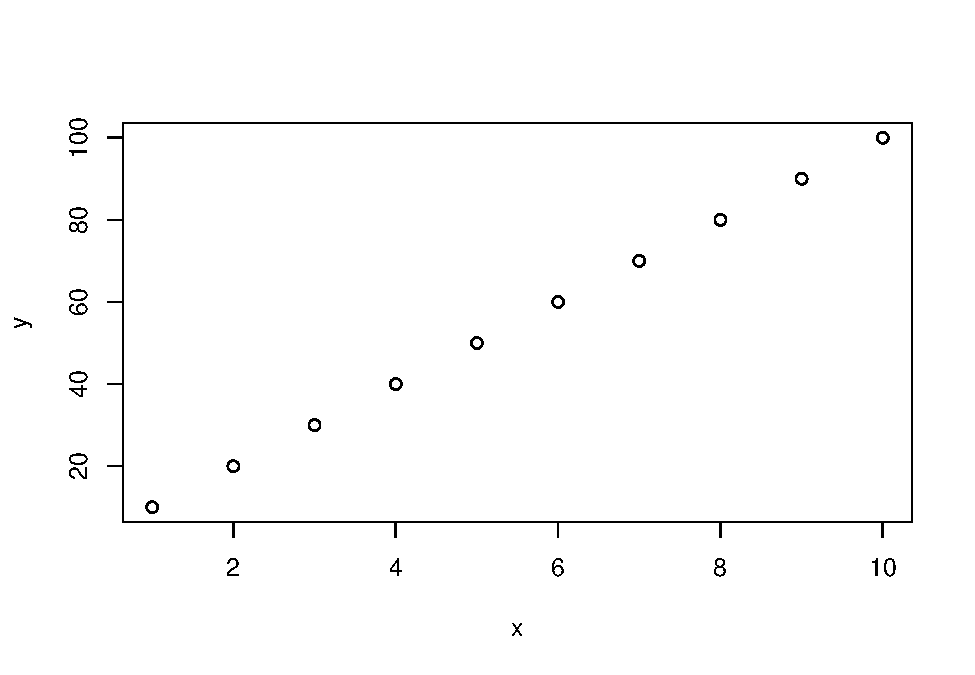
\includegraphics{R_ejercicios2021_files/figure-latex/unnamed-chunk-5-1.pdf}

¿Cuál de los siguientes pasos siguieron para realizar la tarea?\\

Tipeando en la consola

Tipeando en el script y enviando el código a consola (CTRL + R)

Copiando y pegando en consola

Copiando y pegando en el script y enviando el código a consola (CTRL + R)

\hypertarget{r03-buxe1sicos}{%
\chapter*{R03 Básicos}\label{r03-buxe1sicos}}
\addcontentsline{toc}{chapter}{R03 Básicos}

\hypertarget{ayudas-1-rr}{%
\section{Ayudas 1 (RR)}\label{ayudas-1-rr}}

Trabajaremos en este punto con la función \emph{\textbf{median()}} (mediana). Analizar las diferencias entre\\
* ??median

\begin{itemize}
\tightlist
\item
  ?median
\end{itemize}

\begin{itemize}
\tightlist
\item
  apropos(``median'')
\end{itemize}

\hypertarget{ayudas-2-rrr}{%
\section{Ayudas 2 (RRR)}\label{ayudas-2-rrr}}

Averiguar qué hace la siguiente función

\begin{Shaded}
\begin{Highlighting}[]
\KeywordTok{sample}\NormalTok{(}\DecValTok{1}\OperatorTok{:}\DecValTok{10}\NormalTok{, }\DecValTok{20}\NormalTok{, }\DataTypeTok{replace=}\OtherTok{TRUE}\NormalTok{)}
\end{Highlighting}
\end{Shaded}

\hypertarget{cuxf3mputos-rrr}{%
\section{Cómputos (RRR)}\label{cuxf3mputos-rrr}}

\begin{enumerate}
\def\labelenumi{\arabic{enumi}.}
\item
  Calcular en R:

  \[\frac{2^{pi}}{2^{7}}-1\]
\end{enumerate}

\textbf{RTA: -0.9310549 }

\textbf{NOTA:} podemos usar el valor de pi (3.141593) o utilizar la constante pi que trae el R (si es necesario acceder a la ayuda)

\begin{enumerate}
\def\labelenumi{\arabic{enumi}.}
\setcounter{enumi}{1}
\item
  Calcular en R:

  \[\frac{3 - cos({pi})} {\sqrt[2]{7}}\]
\end{enumerate}

\textbf{RTA: 1.5118579 }

\hypertarget{comandos-buxe1sicos-rrr}{%
\section{Comandos básicos (RRR)}\label{comandos-buxe1sicos-rrr}}

Resolver los siguientes puntos

Listar los objetos del workspace

Asignar a un objeto que llamaremos \textbf{\emph{y}} un vector que contenga los números 2, 5, 7, y 9

Aplicar la función \textbf{max()} para obtener el valor máximo del elemento \textbf{\emph{y}}

Reasignar el valor obtenido en el punto anterior al objeto llamado \textbf{\emph{y}} (es decir reescribir \textbf{\emph{y}}) ¿Cuántos elementos tendrá ahora \textbf{\emph{y}}?

\hypertarget{creando-vectores-rr}{%
\section{Creando vectores (RR)}\label{creando-vectores-rr}}

Asignar a un objeto que llamaremos \textbf{\emph{x}} los valores 90, 3, -5

Asignar a un objeto que llamaremos \textbf{\emph{y}} los elementos 90, 3, ``A''. Comparar visualmente los objetos \textbf{\emph{y}} y \textbf{\emph{x}} ¿Se ve alguna diferencia entre ambos objetos?

\hypertarget{nombres-de-objetos-rr}{%
\section{Nombres de objetos (RR)}\label{nombres-de-objetos-rr}}

Identificar cuáles de las siguientes opciones podrían ser utilizadas como nombres de objetos en R. En los casos que sea necesario, proponer cambios para que esos nombres sean aceptados por el programa (lo más parecido posible a los nombres originales)

\begin{itemize}
\tightlist
\item
  RecorCholis\\
\item
  tamaño máximo de célula\\
\item
  SUperficie\_del:Area\\
\item
  4min\\
\item
  site\#7
\item
  sitio?3
\end{itemize}

\hypertarget{operando-con-vectores-rr}{%
\section{Operando con vectores (RR)}\label{operando-con-vectores-rr}}

Crear un objeto llamado \textbf{\emph{zx}} de 100 valores en el \textbf{rango} 100-200. Verificar que el vector creado tenga 100 elementos

Crear un objeto llamado \textbf{\emph{zy}} de dos elementos, con valores 1 y 2

Realizar \textbf{\emph{zx}/\emph{zy}} ¿Qué resultado arroja? ¿Aparece algún mensaje?

Repetir el inciso anterior, pero \textbf{\emph{zy}} tendrán valores 1, 2 y 3

¿Y ahora apareció algún mensaje?

¿Se ejecutó la línea?

Seguramente a esta altura ya han recibido algún triste mensaje de \textbf{\emph{error}}, ¿qué diferencia hay entre un mensaje \textbf{\emph{warning}} y un mensaje \textbf{\emph{error}}?

\hypertarget{dar-nombre-a-los-elementos-de-un-vector-rrr}{%
\section{Dar nombre a los elementos de un vector (RRR)}\label{dar-nombre-a-los-elementos-de-un-vector-rrr}}

Dado el siguiente vector:

\begin{Shaded}
\begin{Highlighting}[]
\NormalTok{miX <-}\StringTok{ }\DecValTok{1}\OperatorTok{:}\DecValTok{15}
\end{Highlighting}
\end{Shaded}

¿Qué resultado dará \textbf{names(miX)}?

\begin{Shaded}
\begin{Highlighting}[]
\KeywordTok{names}\NormalTok{(miX)}
\end{Highlighting}
\end{Shaded}

Sabiendo la respuesta, dar nombres a los elementos de miX, donde a cada elemento se le asignará la letra del abecedario correspondiente a su posición

miX debería verse así:

\begin{verbatim}
 A  B  C  D  E  F  G  H  I  J  K  L  M  N  O 
 1  2  3  4  5  6  7  8  9 10 11 12 13 14 15 
\end{verbatim}

\hypertarget{aplicando-funciones-a-vectores-rr}{%
\section{Aplicando funciones a vectores (RR)}\label{aplicando-funciones-a-vectores-rr}}

Crear un vector \textbf{\emph{y}} con los valores -5, 6, 0, 0, 0, 90, -38. Aplicar una función para convertir todos los valores de \textbf{\emph{y}} a números positivos

Aplicar una función para obtener la mediana de \textbf{\emph{y}}

\hypertarget{pruebas-y-operaciones-luxf3gicas-rrr}{%
\section{Pruebas y operaciones lógicas (RRR)}\label{pruebas-y-operaciones-luxf3gicas-rrr}}

(tomado de swirl(); swirlstats.com)

1 ¿Cuáles de las siguientes expresiones se evaluarán como FALSE?

TRUE \& TRUE

TRUE \& FALSE

FALSE \& TRUE

FALSE \& FALSE

TRUE \textbar{} TRUE

TRUE \textbar{} FALSE

FALSE \textbar{} TRUE

FALSE \textbar{} FALSE

2 ¿Cuál será el resultado y porqué?

TRUE \& c(TRUE, FALSE, FALSE)

TRUE \&\& c(TRUE, FALSE, FALSE)

\hypertarget{pruebas-luxf3gicas}{%
\section{Pruebas lógicas}\label{pruebas-luxf3gicas}}

Dados los siguientes vectores

\begin{Shaded}
\begin{Highlighting}[]
\NormalTok{x <-}\StringTok{ }\KeywordTok{c}\NormalTok{(}\DecValTok{1}\NormalTok{,}\DecValTok{2}\NormalTok{,}\DecValTok{3}\NormalTok{,}\DecValTok{4}\NormalTok{,}\DecValTok{5}\NormalTok{)}
\NormalTok{y <-}\StringTok{ }\KeywordTok{c}\NormalTok{(}\DecValTok{1}\NormalTok{,}\DecValTok{3}\NormalTok{,}\DecValTok{3}\NormalTok{,}\DecValTok{3}\NormalTok{,}\DecValTok{5}\NormalTok{)}
\NormalTok{z <-}\StringTok{ }\KeywordTok{c}\NormalTok{(T,T,T,F,F)}
\NormalTok{k <-}\StringTok{ }\KeywordTok{c}\NormalTok{(T,F,T,F,T)}
\end{Highlighting}
\end{Shaded}

En cada uno de los siguientes casos analizar cual va a ser el resultado y de cuantos elementos estará compuesto el mismo. Luego correr en consola para verificar

\begin{Shaded}
\begin{Highlighting}[]
\NormalTok{x }\OperatorTok{>}\StringTok{ }\DecValTok{3}
\NormalTok{x }\OperatorTok{==}\StringTok{ }\NormalTok{y}
\NormalTok{x }\OperatorTok{!=}\StringTok{ }\NormalTok{y}
\NormalTok{x[}\DecValTok{1}\NormalTok{] }\OperatorTok{==}\StringTok{ }\NormalTok{y[}\DecValTok{1}\NormalTok{]}
\NormalTok{x }\OperatorTok{&&}\StringTok{ }\NormalTok{y}
\NormalTok{z }\OperatorTok{&}\StringTok{ }\NormalTok{k}
\NormalTok{z }\OperatorTok{&&}\StringTok{ }\NormalTok{k}
\NormalTok{z }\OperatorTok{==}\StringTok{ }\NormalTok{k}
\NormalTok{(x }\OperatorTok{>}\StringTok{ }\DecValTok{3} \OperatorTok{&}\StringTok{ }\NormalTok{y }\OperatorTok{>}\StringTok{ }\DecValTok{3}\NormalTok{) }\OperatorTok{|}\StringTok{ }\NormalTok{x }\OperatorTok{==}\StringTok{ }\DecValTok{1}
\NormalTok{x }\OperatorTok{>}\StringTok{ }\DecValTok{3} \OperatorTok{&}\StringTok{ }\NormalTok{y }\OperatorTok{>}\StringTok{ }\DecValTok{3} \OperatorTok{&}\StringTok{ }\NormalTok{z}
\NormalTok{x }\OperatorTok{>}\StringTok{ }\DecValTok{3} \OperatorTok{&}\StringTok{ }\NormalTok{y }\OperatorTok{>}\StringTok{ }\DecValTok{3} \OperatorTok{|}\StringTok{ }\NormalTok{z}
\KeywordTok{any}\NormalTok{(x }\OperatorTok{>}\StringTok{ }\DecValTok{4}\NormalTok{)}
\KeywordTok{any}\NormalTok{ (y }\OperatorTok{>}\StringTok{ }\DecValTok{4}\NormalTok{)}
\KeywordTok{any}\NormalTok{(x }\OperatorTok{>}\StringTok{ }\DecValTok{15} \OperatorTok{|}\StringTok{ }\NormalTok{y }\OperatorTok{>}\StringTok{ }\DecValTok{4}\NormalTok{)}
\KeywordTok{any}\NormalTok{ (x }\OperatorTok{>}\StringTok{ }\DecValTok{15} \OperatorTok{|}\StringTok{ }\NormalTok{y }\OperatorTok{>}\StringTok{ }\DecValTok{5}\NormalTok{)}
\KeywordTok{all}\NormalTok{(x[}\DecValTok{1}\NormalTok{] }\OperatorTok{==}\StringTok{ }\NormalTok{y[}\DecValTok{1}\NormalTok{])}
\KeywordTok{all}\NormalTok{(x[}\DecValTok{1}\NormalTok{] }\OperatorTok{!=}\StringTok{ }\NormalTok{y[}\DecValTok{1}\NormalTok{])}
\end{Highlighting}
\end{Shaded}

\hypertarget{debugging-detectando-errores}{%
\section*{Debugging, detectando errores}\label{debugging-detectando-errores}}
\addcontentsline{toc}{section}{Debugging, detectando errores}

Es importante \textbf{LEER LOS MENSAJES DE ERROR} y \textbf{WARNINGS
}, en la mayoría de los casos son bastante informativos y ayudan a encontrar fallas en el script

Para cada una de las siguientes líneas de código explicar porqué se obtiene un mensaje de error, warnning, o un resultado no esperado.

\begin{Shaded}
\begin{Highlighting}[]
\KeywordTok{rm}\NormalTok{( }\DataTypeTok{list =} \KeywordTok{ls}\NormalTok{() ) }\CommentTok{#eliminemos primero todos los objetos}
\end{Highlighting}
\end{Shaded}

\begin{enumerate}
\def\labelenumi{\arabic{enumi}.}
\item
\end{enumerate}

\begin{Shaded}
\begin{Highlighting}[]
\NormalTok{  y =}\StringTok{ }\KeywordTok{c}\NormalTok{(}\DecValTok{1}\OperatorTok{:}\DecValTok{7}\NormalTok{, }\DecValTok{33}\OperatorTok{/}\NormalTok{(}\DecValTok{2} \OperatorTok{+}\StringTok{ }\DecValTok{5}\NormalTok{)}
\NormalTok{  y}
\end{Highlighting}
\end{Shaded}

\begin{enumerate}
\def\labelenumi{\arabic{enumi}.}
\setcounter{enumi}{1}
\item
\end{enumerate}

\begin{Shaded}
\begin{Highlighting}[]
\NormalTok{  mi_X}
\end{Highlighting}
\end{Shaded}

\begin{enumerate}
\def\labelenumi{\arabic{enumi}.}
\setcounter{enumi}{2}
\item
\end{enumerate}

\begin{Shaded}
\begin{Highlighting}[]
\NormalTok{  myZ <-}\StringTok{ }\NormalTok{(}\DecValTok{1}\NormalTok{,}\DecValTok{4}\NormalTok{,}\DecValTok{5}\NormalTok{,}\DecValTok{7}\NormalTok{)}
\end{Highlighting}
\end{Shaded}

\begin{enumerate}
\def\labelenumi{\arabic{enumi}.}
\setcounter{enumi}{3}
\item
\end{enumerate}

\begin{Shaded}
\begin{Highlighting}[]
  \KeywordTok{mean}\NormalTok{(}\KeywordTok{C}\NormalTok{(x,y))}
\end{Highlighting}
\end{Shaded}

\begin{enumerate}
\def\labelenumi{\arabic{enumi}.}
\setcounter{enumi}{4}
\item
\end{enumerate}

\begin{Shaded}
\begin{Highlighting}[]
\NormalTok{  var}\DecValTok{-3}\NormalTok{ <-}\StringTok{ }\KeywordTok{mean}\NormalTok{(x)}
\end{Highlighting}
\end{Shaded}

\begin{enumerate}
\def\labelenumi{\arabic{enumi}.}
\setcounter{enumi}{5}
\item
\end{enumerate}

\begin{Shaded}
\begin{Highlighting}[]
\NormalTok{  var}\OperatorTok{@}\StringTok{ }\ErrorTok{<}\OperatorTok{-}\StringTok{ }\KeywordTok{mean}\NormalTok{(x)}
\end{Highlighting}
\end{Shaded}

\begin{enumerate}
\def\labelenumi{\arabic{enumi}.}
\setcounter{enumi}{6}
\item
\end{enumerate}

\begin{Shaded}
\begin{Highlighting}[]
  \KeywordTok{sample}\NormalTok{(letters, }\DecValTok{100}\NormalTok{)}
\end{Highlighting}
\end{Shaded}

\hypertarget{r04-indexaciuxf3n-y-filtros}{%
\chapter*{R04 Indexación y Filtros}\label{r04-indexaciuxf3n-y-filtros}}
\addcontentsline{toc}{chapter}{R04 Indexación y Filtros}

\hypertarget{vector-letters-r}{%
\section{Vector LETTERS (R)}\label{vector-letters-r}}

Explorar el objeto LETTERS que viene definido con el paquete básico de R ¿cuántos elementos tiene?

\begin{Shaded}
\begin{Highlighting}[]
\NormalTok{LETTERS}
\end{Highlighting}
\end{Shaded}

\begin{verbatim}
 [1] "A" "B" "C" "D" "E" "F" "G" "H" "I" "J" "K" "L" "M" "N" "O" "P" "Q" "R" "S"
[20] "T" "U" "V" "W" "X" "Y" "Z"
\end{verbatim}

\hypertarget{indexaciuxf3n-de-vectores-rr}{%
\section{Indexación de vectores (RR)}\label{indexaciuxf3n-de-vectores-rr}}

Obtener los 10 primeros elementos de LETTERS

\begin{verbatim}
 [1] "A" "B" "C" "D" "E" "F" "G" "H" "I" "J"
\end{verbatim}

\hypertarget{indexaciuxf3n-de-vectores-rrr}{%
\section{Indexación de vectores (RRR)}\label{indexaciuxf3n-de-vectores-rrr}}

Explicar que hacen las siguientes líneas de comando

\begin{Shaded}
\begin{Highlighting}[]
\NormalTok{miX <-}\StringTok{ }\DecValTok{10}\OperatorTok{:}\DecValTok{1}
\KeywordTok{names}\NormalTok{(miX )}
\end{Highlighting}
\end{Shaded}

\begin{verbatim}
NULL
\end{verbatim}

\begin{Shaded}
\begin{Highlighting}[]
\KeywordTok{names}\NormalTok{(miX ) <-}\StringTok{ }\NormalTok{LETTERS[}\DecValTok{1}\OperatorTok{:}\DecValTok{10}\NormalTok{]}
\end{Highlighting}
\end{Shaded}

\begin{Shaded}
\begin{Highlighting}[]
\NormalTok{miX}
\end{Highlighting}
\end{Shaded}

\begin{verbatim}
##  A  B  C  D  E  F  G  H  I  J 
## 10  9  8  7  6  5  4  3  2  1
\end{verbatim}

\hypertarget{indexaciuxf3n-de-vectores-rrr-1}{%
\section{Indexación de vectores (RRR)}\label{indexaciuxf3n-de-vectores-rrr-1}}

Dado el siguiente vector miX

\begin{verbatim}
 A  B  C  D  E  F  G  H  I  J 
10  9  8  7  6  5  4  3  2  1 
\end{verbatim}

Obtener los cinco primeros elementos de \textbf{\emph{miX}} mediante:\\

Un vector numérico

Un vector con los \textbf{nombres} correspondientes a esos elementos

Un vector lógico

\hypertarget{indexaciuxf3n-de-vectores-rrr-2}{%
\section{Indexación de vectores (RRR)}\label{indexaciuxf3n-de-vectores-rrr-2}}

Explorar el objeto \textbf{\emph{x}} que se da a continuación (Por ahora no importan los comandos que utilizamos para generarlo)

\begin{Shaded}
\begin{Highlighting}[]
  \KeywordTok{set.seed}\NormalTok{(}\DecValTok{300}\NormalTok{)}
\NormalTok{  x <-}\StringTok{ }\KeywordTok{sample}\NormalTok{(}\DecValTok{1}\OperatorTok{:}\DecValTok{100}\NormalTok{, }\DecValTok{40}\NormalTok{, }\DataTypeTok{replace=}\NormalTok{T)}
\end{Highlighting}
\end{Shaded}

Obtener los \textbf{\emph{valores}} de los \textbf{\emph{elementos}} ubicados en las posiciones 5, 10, 15 y 20 de este vector

Generar un nuevo objeto llamado \textbf{\emph{miY}}, repitiendo cuatro veces el primer elemento de \textbf{\emph{x}}, tres veces el segundo elemento y dos veces el tercer elemento. \textbf{\emph{miY}} debería verse así:

\begin{verbatim}
## [1] 78 78 78 78 66 66 66 89 89
\end{verbatim}

\hypertarget{indexaciuxf3n-uxedndices-luxf3gicos-vs-which-rrr}{%
\section{Indexación: índices lógicos vs which (RRR)}\label{indexaciuxf3n-uxedndices-luxf3gicos-vs-which-rrr}}

Explorar el objeto \textbf{\emph{x}} que se da a continuación

\begin{Shaded}
\begin{Highlighting}[]
  \KeywordTok{set.seed}\NormalTok{(}\DecValTok{300}\NormalTok{)}
\NormalTok{  x <-}\StringTok{ }\KeywordTok{sample}\NormalTok{(}\DecValTok{1}\OperatorTok{:}\DecValTok{100}\NormalTok{, }\DecValTok{40}\NormalTok{, }\DataTypeTok{replace=}\NormalTok{ T)}
\end{Highlighting}
\end{Shaded}

Generar un vector lógico, que llamaremos \textbf{\emph{idx1}}. El mismo tomará valores {T} para aquellos valores de \textbf{\emph{x}} mayores o iguales a 20 y {F} para los valores de \textbf{\emph{x}} menores a 20

Utilizar el objeto \textbf{\emph{idx1}} recién generado para obtener los \textbf{valores} del vector \textbf{\emph{x}} mayores o iguales a 20

Utilizando la función \textbf{which()}, obtener la \textbf{posición} de los elementos de \textbf{\emph{x}} cuyos valores sean mayores o iguales a 20. Asignar la salida de la función a un objeto que llamaremos \textbf{\emph{idx2}}

Utilizar el objeto \textbf{\emph{idx2}} recién generado para obtener los \textbf{valores} del vector \textbf{\emph{x}} mayores o iguales a 20

El resultado obtenido fue el mismo cuando indexamos con el vector lógico (\textbf{\emph{idx1}}) y cuando usamos la función which (\textbf{\emph{idx2}}). Sin embargo, \textbf{\emph{idx1}} tiene 40 elementos, mientras que \textbf{\emph{idx2}} tiene 33 elementos ¿por qué?

\hypertarget{indexaciuxf3n-en-vectores-ejemplo-colors-rrr}{%
\section{Indexación en vectores ejemplo colors() (RRR)}\label{indexaciuxf3n-en-vectores-ejemplo-colors-rrr}}

Escribir \textbf{colors()} en consola para examinar el objeto

¿Qué diferencia estructural hay entre los objetos colors y letters? Recurrir a la ayuda si fuera necesario

Volveremos a utilizar este objeto en varias ocasiones durante el curso. Por ahora simplemente lo usaremos como ejemplo.

\begin{Shaded}
\begin{Highlighting}[]
\KeywordTok{colors}\NormalTok{()}
\end{Highlighting}
\end{Shaded}

Asignar el objeto \textbf{colors()} a un nuevo objeto que llamaremos \textbf{\emph{misColores}}

Generar un objeto, al que llamaremos \textbf{\emph{amarillos}}, con aquellos elementos de \textbf{\emph{misColores}} que contengan en alguna parte del texto la palabra ``yellow''

¿Cuántos elementos tiene el objeto \textbf{\emph{amarillos}}?

Para generar el objeto \textbf{\emph{amarillos}} ¿era necesario generar el objeto \textbf{\emph{misColores}}?

\hypertarget{debugging-detectando-errores-1}{%
\section*{Debugging, detectando errores}\label{debugging-detectando-errores-1}}
\addcontentsline{toc}{section}{Debugging, detectando errores}

Para cada una de las siguientes líneas de código explicar porqué se obtiene un mensaje de error, warnning, o un resultado no esperado

\begin{Shaded}
\begin{Highlighting}[]
\KeywordTok{rm}\NormalTok{( }\DataTypeTok{list =} \KeywordTok{ls}\NormalTok{() ) }\CommentTok{#eliminemos primero todos los objetos}
\end{Highlighting}
\end{Shaded}

\begin{enumerate}
\def\labelenumi{\arabic{enumi}.}
\item
\end{enumerate}

\begin{Shaded}
\begin{Highlighting}[]
\NormalTok{k <-}\StringTok{ }\KeywordTok{letters}\NormalTok{(}\DecValTok{1}\NormalTok{)}
\end{Highlighting}
\end{Shaded}

\begin{enumerate}
\def\labelenumi{\arabic{enumi}.}
\setcounter{enumi}{1}
\item
\end{enumerate}

\begin{Shaded}
\begin{Highlighting}[]
\KeywordTok{month.name}\NormalTok{(}\DecValTok{1}\OperatorTok{:}\DecValTok{10}\NormalTok{)}
\end{Highlighting}
\end{Shaded}

\begin{enumerate}
\def\labelenumi{\arabic{enumi}.}
\setcounter{enumi}{2}
\item
\end{enumerate}

\begin{Shaded}
\begin{Highlighting}[]
\NormalTok{y <-}\StringTok{ }\KeywordTok{c}\NormalTok{(}\StringTok{"A"}\NormalTok{, }\StringTok{"B"}\NormalTok{, }\StringTok{"C"}\NormalTok{, }\StringTok{"D"}\NormalTok{)}
\NormalTok{txt <-}\StringTok{ }\NormalTok{letters[y]}
\end{Highlighting}
\end{Shaded}

\hypertarget{r05-workspace-y-rhistory}{%
\chapter*{R05 Workspace y RHistory}\label{r05-workspace-y-rhistory}}
\addcontentsline{toc}{chapter}{R05 Workspace y RHistory}

\hypertarget{responder-con-verdadero-o-falso-rrr}{%
\section{Responder con Verdadero o Falso (RRR)}\label{responder-con-verdadero-o-falso-rrr}}

El working directory siempre es el directorio donde tenemos guardado el script

Todos los scripts deben estar guardados en la misma ubicación que el directorio de trabajo

El Rstudio tiene definido un directorio de trabajo por defecto

En una sesión de R sólo puede haber un directorio de trabajo. Sin embargo en un script se puede re-definir el directorio de trabajo tantas veces como uno quiera

Hice una simulación que tardó 3 hs en correr y no guardé los objetos generados. No me preocupo porque el resultado siempre se guarda en el Rhistory

Hice una simulación que tardó 3 hs en correr y no guardé los objetos generados, pero no me preocupo porque el resultado siempre se guarda en el RData

Por defecto (default) R genera el RHistory, donde guarda los comandos y objetos generados en la última sesión

En el RHistory quedan registrados los pasos en el mismo orden que aparecen en el script

Podemos selectivamente guardar un único objeto y cargarlo cuando lo necesitemos

El comando ``ctrl + l'' aplicado a la consola (clear console, limpiar consola) tiene el mismo efecto que remover los objetos rm( list= ls() )

\hypertarget{salvar-y-cargar-objetos-rr}{%
\section{Salvar y cargar objetos (RR)}\label{salvar-y-cargar-objetos-rr}}

Correr la siguiente línea para remover todos los objetos creados durante esta sesión

\begin{Shaded}
\begin{Highlighting}[]
\KeywordTok{rm}\NormalTok{( }\DataTypeTok{list =} \KeywordTok{ls}\NormalTok{() )}
\end{Highlighting}
\end{Shaded}

Comprobar que no hay objetos en nuestra sesión

\begin{Shaded}
\begin{Highlighting}[]
\KeywordTok{ls}\NormalTok{()}
\end{Highlighting}
\end{Shaded}

\begin{verbatim}
## character(0)
\end{verbatim}

Dados los siguientes objetos

\begin{Shaded}
\begin{Highlighting}[]
\NormalTok{y <-}\StringTok{ }\KeywordTok{rnorm}\NormalTok{(}\DecValTok{100}\NormalTok{)}
\NormalTok{x <-}\StringTok{ }\DecValTok{1}\OperatorTok{:}\DecValTok{10}
\NormalTok{z <-}\StringTok{ }\NormalTok{letters}
\end{Highlighting}
\end{Shaded}

Guardar la sesión de trabajo

Guardar solamente los objetos x, y

Remover todos los objetos y volver a cargar solamente x

Pedir un listado de todos los objetos

\hypertarget{debugging-detectando-errores-2}{%
\section{Debugging, detectando errores}\label{debugging-detectando-errores-2}}

Para cada una de las siguientes líneas de código explicar porqué se obtiene un mensaje de error, warnning, o un resultado no esperado

\begin{Shaded}
\begin{Highlighting}[]
\KeywordTok{rm}\NormalTok{( }\DataTypeTok{list =} \KeywordTok{ls}\NormalTok{() ) }\CommentTok{#eliminemos primero todos los objetos}
\end{Highlighting}
\end{Shaded}

\begin{enumerate}
\def\labelenumi{\arabic{enumi}.}
\item
\end{enumerate}

\begin{Shaded}
\begin{Highlighting}[]
\KeywordTok{setwd}\NormalTok{(}\StringTok{"C:\textbackslash{}R2021/R_Archivos/"}\NormalTok{)}
\end{Highlighting}
\end{Shaded}

\begin{enumerate}
\def\labelenumi{\arabic{enumi}.}
\setcounter{enumi}{1}
\item
\end{enumerate}

\begin{Shaded}
\begin{Highlighting}[]
\KeywordTok{setwd}\NormalTok{(C}\OperatorTok{:}\ErrorTok{/}\NormalTok{R2021}\OperatorTok{/}\NormalTok{R_Archivos}\OperatorTok{/}\NormalTok{)}
\end{Highlighting}
\end{Shaded}

\hypertarget{r06-importar-y-exportar}{%
\chapter*{R06 Importar y Exportar}\label{r06-importar-y-exportar}}
\addcontentsline{toc}{chapter}{R06 Importar y Exportar}

\hypertarget{responder-con-verdadero-o-falso-rrr-1}{%
\section{Responder con Verdadero o Falso (RRR)}\label{responder-con-verdadero-o-falso-rrr-1}}

Los archivos que se quieren cargar (read.table) deben estar en el mismo directorio de trabajo que el script que los carga

Los campos de un archivo a importar siempre deben estar separados por comas

Para importar un archivo el separador decimal siempre tiene que ser el punto (``.'')

Tanto los archivos de entrada como los de salida tienen que tener definidos los nombres de filas y columnas

Al importar una tabla los cambios generados en R no modificarán los datos contenidos en el archivo de origen

Una ruta absoluta es aquella que especifica la ubicación de una carpeta o archivo desde su directorio raíz

Para ser importados a R los datos siempre deben estar ordenados en un sistema de filas y columnas

Para importar una tabla con encabezados, todas las columnas deben estar nombradas

Si importamos una tabla con nombres de encabezado repetidos R renombrará cada encabezado para que éstos no tengan nombres repetidos

Siempre hay que ingresar la ruta absoluta del archivo a importar o a exportar

\hypertarget{read.table-y-write.table}{%
\section{read.table y write.table}\label{read.table-y-write.table}}

Con un editor de texto (ej bloc de notas, o el propio Rstudio) abrir los archivos ``MiTrayect1.csv'' y ``MiTrayect2.csv'', alojados en la carpeta ``4-Datos''. Identificar el separador de campos y el símbolo decimal. Los datos son posiciones geográficas de una determinada trayectoria

Importar a R (\textbf{\emph{read.table()}}) ambos arvhivos, asignando el resultado de la importación a dos objetos que llamaremos respectivamente \emph{tray1} y \emph{tray2}

Mostrar en consola ambos objetos para ver su estructura

Generar un objeto al que llamaremos ``tray3'' combinando los dos objetos recién creados. El nuevo objeto deberá tener dos columnas (dlon y dlat) y tantas filas como la suma de las filas de los dos archivos recién incorporados.

Usar la función \textbf{rbind()} (row binding, juntar por filas) para ``juntar'' ambas series de datos en una sola tabla. La función se usa:

\begin{Shaded}
\begin{Highlighting}[]
\KeywordTok{rbind}\NormalTok{ (x, y)}
\end{Highlighting}
\end{Shaded}

Guardar en la carpeta ``Resultados'' (\textbf{\emph{write.table()}}) un archivo de texto con el contenido de \emph{\textbf{tray3}} con el nombre ``Trayect1+2.csv''. Asegurarse que el archivo de salida tenga el mismo formato que los archivos originales (nombres de columnas, separadores de campos, símbolo decimal, sin nombre de filas, etc.)

\hypertarget{debugging-detectando-errores-3}{%
\section{Debugging, detectando errores}\label{debugging-detectando-errores-3}}

Para cada una de las siguientes líneas de código explicar porqué se obtiene un mensaje de error, warnning, o un resultado no esperado

\begin{Shaded}
\begin{Highlighting}[]
\KeywordTok{rm}\NormalTok{( }\DataTypeTok{list =} \KeywordTok{ls}\NormalTok{() ) }\CommentTok{#eliminemos primero todos los objetos}
\end{Highlighting}
\end{Shaded}

\begin{Shaded}
\begin{Highlighting}[]
\CommentTok{#Generamos un objeto de prueba}
\NormalTok{x <-}\StringTok{ }\DecValTok{1}\OperatorTok{:}\DecValTok{100}
\end{Highlighting}
\end{Shaded}

\begin{enumerate}
\def\labelenumi{\arabic{enumi}.}
\item
\end{enumerate}

\begin{Shaded}
\begin{Highlighting}[]
\KeywordTok{read.table}\NormalTok{(c}\OperatorTok{:}\ErrorTok{/}\NormalTok{R2015}\OperatorTok{/}\NormalTok{R_Archivos}\OperatorTok{/}\DecValTok{4}\OperatorTok{-}\NormalTok{Datos}\OperatorTok{/}\NormalTok{MiTrayect1.csv, }\DataTypeTok{sep=} \StringTok{","}\NormalTok{, }\DataTypeTok{dec=} \StringTok{"."}\NormalTok{, }\DataTypeTok{header=}\NormalTok{ T )}
\end{Highlighting}
\end{Shaded}

\begin{enumerate}
\def\labelenumi{\arabic{enumi}.}
\setcounter{enumi}{1}
\item
\end{enumerate}

\begin{Shaded}
\begin{Highlighting}[]
\KeywordTok{read.table}\NormalTok{(}\StringTok{"C:/R2015/R_Archivos/4-Datos/MiTrayect1.csv"}\NormalTok{, }\DataTypeTok{sep=} \StringTok{","}\NormalTok{, }\DataTypeTok{dec=} \StringTok{"."}\NormalTok{, }\DataTypeTok{header=} \StringTok{"T"}\NormalTok{ )}
\end{Highlighting}
\end{Shaded}

\begin{enumerate}
\def\labelenumi{\arabic{enumi}.}
\setcounter{enumi}{2}
\item
\end{enumerate}

\begin{Shaded}
\begin{Highlighting}[]
\KeywordTok{write.table}\NormalTok{(}\StringTok{"C:/R2015/R_Archivos/Resultados/nombre.csv"}\NormalTok{, }\DataTypeTok{sep=} \StringTok{","}\NormalTok{, }\DataTypeTok{dec=} \StringTok{"."}\NormalTok{)}
\end{Highlighting}
\end{Shaded}

\begin{enumerate}
\def\labelenumi{\arabic{enumi}.}
\setcounter{enumi}{3}
\item
\end{enumerate}

\begin{Shaded}
\begin{Highlighting}[]
\KeywordTok{write.table}\NormalTok{(x, }\StringTok{"C:/R2015/R_Archivos/Resultados/nombre.csv"}\NormalTok{, }\DataTypeTok{sep=} \StringTok{","}\NormalTok{, }\DataTypeTok{dec=} \StringTok{"."}\NormalTok{, }\DataTypeTok{header=}\NormalTok{ T)}
\end{Highlighting}
\end{Shaded}

\begin{enumerate}
\def\labelenumi{\arabic{enumi}.}
\setcounter{enumi}{4}
\item
\end{enumerate}

\begin{Shaded}
\begin{Highlighting}[]
\KeywordTok{write.table}\NormalTok{(x }\StringTok{"C:/R2015/R_Archivos/Resultados/nombre.csv"}\NormalTok{, }\DataTypeTok{sep=} \StringTok{","}\NormalTok{, }\DataTypeTok{dec=} \StringTok{"."}\NormalTok{)}
\end{Highlighting}
\end{Shaded}

\hypertarget{r07-objetos-1}{%
\chapter*{R07 Objetos 1}\label{r07-objetos-1}}
\addcontentsline{toc}{chapter}{R07 Objetos 1}

\hypertarget{vectores-1-rr}{%
\section{Vectores 1 (RR)}\label{vectores-1-rr}}

\begin{enumerate}
\def\labelenumi{\arabic{enumi}.}
\tightlist
\item
  Generar cinco vectores de \textbf{10 elementos} cada uno con los nombres y características que se dan a continuación. Utilizar las funciones \textbf{seq()} y \textbf{rep()} en los casos pertinentes.
\end{enumerate}

\begin{itemize}
\tightlist
\item
  texto: un vector texto con las 10 primeras letras del abecedario
\end{itemize}

\begin{Shaded}
\begin{Highlighting}[]
\NormalTok{texto}
\end{Highlighting}
\end{Shaded}

\begin{verbatim}
 [1] "A" "B" "C" "D" "E" "F" "G" "H" "I" "J"
\end{verbatim}

\begin{itemize}
\tightlist
\item
  enteros: primeros 10 números impares
\end{itemize}

\begin{Shaded}
\begin{Highlighting}[]
\NormalTok{enteros }
\end{Highlighting}
\end{Shaded}

\begin{verbatim}
 [1]  1  3  5  7  9 11 13 15 17 19
\end{verbatim}

\begin{itemize}
\tightlist
\item
  decimales: valores entre 1 y 1.9 en intervalos de 0.1
\end{itemize}

\begin{Shaded}
\begin{Highlighting}[]
\NormalTok{decimales }
\end{Highlighting}
\end{Shaded}

\begin{verbatim}
 [1] 1.0 1.1 1.2 1.3 1.4 1.5 1.6 1.7 1.8 1.9
\end{verbatim}

\begin{itemize}
\tightlist
\item
  lógico: 5 valores T seguidos de 5 F
\end{itemize}

\begin{Shaded}
\begin{Highlighting}[]
\NormalTok{logico }
\end{Highlighting}
\end{Shaded}

\begin{verbatim}
 [1]  TRUE  TRUE  TRUE  TRUE  TRUE FALSE FALSE FALSE FALSE FALSE
\end{verbatim}

\begin{itemize}
\tightlist
\item
  factor1: un vector tipo factor con las 10 primeras letras del abecedario
\end{itemize}

\begin{Shaded}
\begin{Highlighting}[]
\NormalTok{factor1}
\end{Highlighting}
\end{Shaded}

\begin{verbatim}
 [1] a b c d e f g h i j
Levels: a b c d e f g h i j
\end{verbatim}

\begin{itemize}
\tightlist
\item
  factor2: el mismo objeto que el punto anterior pero con orden de jerarquía, donde a \textgreater{} b \textgreater{} c\ldots{}. \textgreater{}j
\end{itemize}

\begin{Shaded}
\begin{Highlighting}[]
\NormalTok{factor2}
\end{Highlighting}
\end{Shaded}

\begin{verbatim}
 [1] a b c d e f g h i j
Levels: j < i < h < g < f < e < d < c < b < a
\end{verbatim}

\begin{enumerate}
\def\labelenumi{\arabic{enumi}.}
\setcounter{enumi}{1}
\tightlist
\item
  Comparar la salida en consola de cada uno de los objetos
\end{enumerate}

\hypertarget{vectores-2-rr}{%
\section{Vectores 2 (RR)}\label{vectores-2-rr}}

¿Cuál es el error en las siguientes lineas de comando?

\begin{Shaded}
\begin{Highlighting}[]
\NormalTok{miX <-}\StringTok{ }\NormalTok{(}\StringTok{"uno"}\NormalTok{, }\StringTok{"dos"}\NormalTok{, }\StringTok{"tres"}\NormalTok{)}

\NormalTok{miY <-}\StringTok{ }\KeywordTok{c}\NormalTok{(uno, dos, tres)}

\NormalTok{miZ <-}\StringTok{ "a"}\OperatorTok{:}\StringTok{"Z"}
\end{Highlighting}
\end{Shaded}

\hypertarget{r08-objetos2}{%
\chapter*{R08 Objetos2}\label{r08-objetos2}}
\addcontentsline{toc}{chapter}{R08 Objetos2}

\hypertarget{responder-con-verdadero-o-falso-rrr-2}{%
\section{Responder con verdadero o falso (RRR)}\label{responder-con-verdadero-o-falso-rrr-2}}

\begin{enumerate}
\def\labelenumi{\arabic{enumi}.}
\tightlist
\item
  Tanto las matrices como los data.frame son arreglos rectangulares de datos. Lo que significa que están formados por uno o más vectores de iguales dimensiones y todos los elementos que los componen tienen datos o valores NA
\item
  A diferencia de los data.frame, las matrices tienen el mismo número de filas que de columnas
\item
  Todos los vectores que componen una matriz deben tener el mismo formato (numérico, texto o lógico), aunque también pueden incluir NA's o ser de NA's únicamente
\item
  Los data.frame permiten que un mismo vector-columna contenga datos con más de un tipo de formato
\item
  Un array \textbf{puede pensarse} como un vector con n elementos, donde cada elemento es una matriz y todas las matrices tienen las mismas dimensiones
\item
  Las listas, arrays, matrices y data.frames tienen las mismas dimensiones
\item
  El objeto par() es una lista
\item
  El siguiente objeto x es un data frame de una fila y 10 columnas
\end{enumerate}

\begin{Shaded}
\begin{Highlighting}[]
\NormalTok{x <-}\StringTok{ }\DecValTok{1}\OperatorTok{:}\DecValTok{10}
    \KeywordTok{names}\NormalTok{(x) <-}\StringTok{ }\NormalTok{letters[}\DecValTok{1}\OperatorTok{:}\DecValTok{10}\NormalTok{]}
\NormalTok{        x}
\end{Highlighting}
\end{Shaded}

\begin{verbatim}
 a  b  c  d  e  f  g  h  i  j 
 1  2  3  4  5  6  7  8  9 10 
\end{verbatim}

\begin{enumerate}
\def\labelenumi{\arabic{enumi}.}
\setcounter{enumi}{8}
\tightlist
\item
  La siguiente es una matriz compuesta por una columna de datos con formato numérico y una columna de texto
\end{enumerate}

\begin{Shaded}
\begin{Highlighting}[]
\KeywordTok{matrix}\NormalTok{(}\KeywordTok{c}\NormalTok{(}\DecValTok{1}\OperatorTok{:}\DecValTok{3}\NormalTok{,}\StringTok{"a"}\NormalTok{, }\StringTok{"b"}\NormalTok{,}\StringTok{"c"}\NormalTok{), }\DataTypeTok{ncol=}\DecValTok{2}\NormalTok{)}
\end{Highlighting}
\end{Shaded}

\begin{verbatim}
     [,1] [,2]
[1,] "1"  "a" 
[2,] "2"  "b" 
[3,] "3"  "c" 
\end{verbatim}

\begin{enumerate}
\def\labelenumi{\arabic{enumi}.}
\setcounter{enumi}{9}
\tightlist
\item
  Las dimensiones de un data.frame difieren si al mismo se le agrega nombre de filas (rownames)
\end{enumerate}

\hypertarget{generar-un-data.frame-1-r}{%
\section{Generar un data.frame 1 (R)}\label{generar-un-data.frame-1-r}}

Con los siguientes vectores crear un objeto del tipo data.frame, al que llamaremos \emph{MiDf}.

\begin{Shaded}
\begin{Highlighting}[]
\NormalTok{letras <-}\StringTok{ }\NormalTok{LETTERS[}\DecValTok{1}\OperatorTok{:}\DecValTok{10}\NormalTok{]  }
\NormalTok{enteros <-}\StringTok{ }\KeywordTok{round}\NormalTok{( }\KeywordTok{runif}\NormalTok{(}\DecValTok{10}\NormalTok{, }\DecValTok{0}\NormalTok{, }\DecValTok{10}\NormalTok{), }\DecValTok{0}\NormalTok{ )  }
\NormalTok{decimales <-}\StringTok{ }\KeywordTok{round}\NormalTok{( }\KeywordTok{runif}\NormalTok{(}\DecValTok{10}\NormalTok{, }\DecValTok{0}\NormalTok{, }\DecValTok{10}\NormalTok{), }\DecValTok{3}\NormalTok{ )  }
\NormalTok{logicos <-}\StringTok{ }\KeywordTok{sample}\NormalTok{( }\KeywordTok{c}\NormalTok{(T,F), }\DecValTok{10}\NormalTok{, }\DataTypeTok{replace=}\NormalTok{T ) }
\end{Highlighting}
\end{Shaded}

\begin{Shaded}
\begin{Highlighting}[]
\NormalTok{MiDf}
\end{Highlighting}
\end{Shaded}

\begin{verbatim}
   letras enteros decimales logicos
1       A       4     6.638    TRUE
2       B       1     7.662   FALSE
3       C       3     0.350    TRUE
4       D       9     0.390    TRUE
5       E       0     9.803   FALSE
6       F       3     2.716   FALSE
7       G       6     0.483   FALSE
8       H       8     6.413   FALSE
9       I       4     4.885    TRUE
10      J       2     2.722   FALSE
\end{verbatim}

\hypertarget{agregar-columnas-a-un-data.frame-rr}{%
\section{Agregar columnas a un data.frame (RR)}\label{agregar-columnas-a-un-data.frame-rr}}

Agregar al data frame del punto anterior una columna con valores NA's. A esta columna la llamaremos \emph{sin.dato}

\begin{Shaded}
\begin{Highlighting}[]
\NormalTok{MiDf}
\end{Highlighting}
\end{Shaded}

\begin{verbatim}
   letras enteros decimales logicos sin.dato
1       A       4     6.638    TRUE       NA
2       B       1     7.662   FALSE       NA
3       C       3     0.350    TRUE       NA
4       D       9     0.390    TRUE       NA
5       E       0     9.803   FALSE       NA
6       F       3     2.716   FALSE       NA
7       G       6     0.483   FALSE       NA
8       H       8     6.413   FALSE       NA
9       I       4     4.885    TRUE       NA
10      J       2     2.722   FALSE       NA
\end{verbatim}

\hypertarget{generar-un-data.frame-2-seq-rep-paste-rrr}{%
\section{Generar un data.frame 2: seq(), rep(), paste() (RRR)}\label{generar-un-data.frame-2-seq-rep-paste-rrr}}

Utilizar una combinación de funciones \textbf{rep()}, \textbf{paste()}, \textbf{seq()} y \textbf{data.frame()} para generar una tabla similar a la que se muestra a continuación:

\begin{verbatim}
     tratamiento dosis resultado
1  tratamiento 1     0        NA
2  tratamiento 1     1        NA
3  tratamiento 1    10        NA
4  tratamiento 1   100        NA
5  tratamiento 1  1000        NA
6  tratamiento 3     0        NA
7  tratamiento 3     1        NA
8  tratamiento 3    10        NA
9  tratamiento 3   100        NA
10 tratamiento 3  1000        NA
11 tratamiento 5     0        NA
12 tratamiento 5     1        NA
13 tratamiento 5    10        NA
14 tratamiento 5   100        NA
15 tratamiento 5  1000        NA
16 tratamiento 7     0        NA
17 tratamiento 7     1        NA
18 tratamiento 7    10        NA
19 tratamiento 7   100        NA
20 tratamiento 7  1000        NA
21 tratamiento 9     0        NA
22 tratamiento 9     1        NA
23 tratamiento 9    10        NA
24 tratamiento 9   100        NA
25 tratamiento 9  1000        NA
\end{verbatim}

Nota 1: los valores 1 a 15 no forman parte de la tabla, son los indicadores del nro de fila que da la consola de R
Nota 2: la secuencia dosis puede generarse a partir del siguiente vector

\begin{Shaded}
\begin{Highlighting}[]
\NormalTok{dosis <-}\StringTok{ }\KeywordTok{c}\NormalTok{(}\DecValTok{0}\NormalTok{,}\DecValTok{1}\NormalTok{,}\DecValTok{10}\NormalTok{,}\DecValTok{100}\NormalTok{,}\DecValTok{1000}\NormalTok{)}
\end{Highlighting}
\end{Shaded}

Nota 3: es conveniente aprovechar la regla de reciclado de vectores

\hypertarget{sort-vs-order-rr}{%
\section{sort vs order (RR)}\label{sort-vs-order-rr}}

Dado el siguiente vector

\begin{Shaded}
\begin{Highlighting}[]
\NormalTok{miX <-}\StringTok{ }\DecValTok{15}\OperatorTok{:}\DecValTok{1}
\KeywordTok{names}\NormalTok{(miX) <-}\StringTok{ }\NormalTok{letters[}\DecValTok{1}\OperatorTok{:}\DecValTok{15}\NormalTok{]}
\NormalTok{miX }
\end{Highlighting}
\end{Shaded}

\begin{verbatim}
##  a  b  c  d  e  f  g  h  i  j  k  l  m  n  o 
## 15 14 13 12 11 10  9  8  7  6  5  4  3  2  1
\end{verbatim}

Ordenar en forma ascendente el vector \textbf{\emph{miX}} utilizando:\\
* La función \textbf{sort()}\\
* La función \textbf{order()}

\begin{verbatim}
 o  n  m  l  k  j  i  h  g  f  e  d  c  b  a 
 1  2  3  4  5  6  7  8  9 10 11 12 13 14 15 
\end{verbatim}

\hypertarget{ordenar-un-data.frame-rrr}{%
\section{Ordenar un data.frame (RRR)}\label{ordenar-un-data.frame-rrr}}

La utilidad de \emph{\textbf{order()}} es más evidente cuando queremos ordenar un data.frame.
Dado el siguiente data.frame

\begin{Shaded}
\begin{Highlighting}[]
\NormalTok{trat <-}\StringTok{ }\KeywordTok{paste}\NormalTok{(}\StringTok{"tratamiento"}\NormalTok{, }\KeywordTok{rep}\NormalTok{( }\KeywordTok{seq}\NormalTok{(}\DecValTok{1}\NormalTok{, }\DecValTok{9}\NormalTok{, }\DecValTok{2}\NormalTok{), }\DataTypeTok{each=}\DecValTok{5}\NormalTok{))}
\NormalTok{dosis <-}\StringTok{ }\KeywordTok{c}\NormalTok{(}\DecValTok{0}\NormalTok{,}\DecValTok{1}\NormalTok{,}\DecValTok{10}\NormalTok{,}\DecValTok{100}\NormalTok{,}\DecValTok{1000}\NormalTok{)}
\NormalTok{tabla <-}\StringTok{ }\KeywordTok{data.frame}\NormalTok{(}\DataTypeTok{tratamiento=}\NormalTok{ trat, }\DataTypeTok{dosis=}\NormalTok{ dosis, }\DataTypeTok{resultado=} \OtherTok{NA}\NormalTok{)}
\NormalTok{tabla}
\end{Highlighting}
\end{Shaded}

\begin{verbatim}
##      tratamiento dosis resultado
## 1  tratamiento 1     0        NA
## 2  tratamiento 1     1        NA
## 3  tratamiento 1    10        NA
## 4  tratamiento 1   100        NA
## 5  tratamiento 1  1000        NA
## 6  tratamiento 3     0        NA
## 7  tratamiento 3     1        NA
## 8  tratamiento 3    10        NA
## 9  tratamiento 3   100        NA
## 10 tratamiento 3  1000        NA
## 11 tratamiento 5     0        NA
## 12 tratamiento 5     1        NA
## 13 tratamiento 5    10        NA
## 14 tratamiento 5   100        NA
## 15 tratamiento 5  1000        NA
## 16 tratamiento 7     0        NA
## 17 tratamiento 7     1        NA
## 18 tratamiento 7    10        NA
## 19 tratamiento 7   100        NA
## 20 tratamiento 7  1000        NA
## 21 tratamiento 9     0        NA
## 22 tratamiento 9     1        NA
## 23 tratamiento 9    10        NA
## 24 tratamiento 9   100        NA
## 25 tratamiento 9  1000        NA
\end{verbatim}

Utilizar la función order() para ordenar el objeto \emph{tabla} en orden creciente de la variable \emph{dosis} como se muestra a continuación

\begin{verbatim}
     tratamiento dosis resultado
1  tratamiento 1     0        NA
6  tratamiento 3     0        NA
11 tratamiento 5     0        NA
16 tratamiento 7     0        NA
21 tratamiento 9     0        NA
2  tratamiento 1     1        NA
7  tratamiento 3     1        NA
12 tratamiento 5     1        NA
17 tratamiento 7     1        NA
22 tratamiento 9     1        NA
3  tratamiento 1    10        NA
8  tratamiento 3    10        NA
13 tratamiento 5    10        NA
18 tratamiento 7    10        NA
23 tratamiento 9    10        NA
4  tratamiento 1   100        NA
9  tratamiento 3   100        NA
14 tratamiento 5   100        NA
19 tratamiento 7   100        NA
24 tratamiento 9   100        NA
5  tratamiento 1  1000        NA
10 tratamiento 3  1000        NA
15 tratamiento 5  1000        NA
20 tratamiento 7  1000        NA
25 tratamiento 9  1000        NA
\end{verbatim}

\hypertarget{generar-matrices-rr}{%
\section{Generar matrices (RR)}\label{generar-matrices-rr}}

\begin{enumerate}
\def\labelenumi{\arabic{enumi}.}
\tightlist
\item
  Generar dos matrices (\emph{MiMz1} y \emph{MiMz2}) de dos columnas y 100 filas con números del 1 al 200. En la primera los números deberán llenarse por filas y en la segunda por columnas
\end{enumerate}

\begin{Shaded}
\begin{Highlighting}[]
\KeywordTok{head}\NormalTok{(MiMz1)}
\end{Highlighting}
\end{Shaded}

\begin{verbatim}
     [,1] [,2]
[1,]    1    2
[2,]    3    4
[3,]    5    6
[4,]    7    8
[5,]    9   10
[6,]   11   12
\end{verbatim}

\begin{Shaded}
\begin{Highlighting}[]
\KeywordTok{head}\NormalTok{(MiMz2)}
\end{Highlighting}
\end{Shaded}

\begin{verbatim}
     [,1] [,2]
[1,]    1  101
[2,]    2  102
[3,]    3  103
[4,]    4  104
[5,]    5  105
[6,]    6  106
\end{verbatim}

\begin{enumerate}
\def\labelenumi{\arabic{enumi}.}
\setcounter{enumi}{1}
\tightlist
\item
  Ahora generar una matriz (\emph{MNa}) de 10 columnas cada una con 100 elementos con valores NA
\end{enumerate}

\begin{Shaded}
\begin{Highlighting}[]
\KeywordTok{head}\NormalTok{(MNa)}
\end{Highlighting}
\end{Shaded}

\begin{verbatim}
     [,1] [,2] [,3] [,4] [,5] [,6] [,7] [,8] [,9] [,10]
[1,]   NA   NA   NA   NA   NA   NA   NA   NA   NA    NA
[2,]   NA   NA   NA   NA   NA   NA   NA   NA   NA    NA
[3,]   NA   NA   NA   NA   NA   NA   NA   NA   NA    NA
[4,]   NA   NA   NA   NA   NA   NA   NA   NA   NA    NA
[5,]   NA   NA   NA   NA   NA   NA   NA   NA   NA    NA
[6,]   NA   NA   NA   NA   NA   NA   NA   NA   NA    NA
\end{verbatim}

\hypertarget{combinar-matrices-rr}{%
\section{Combinar matrices (RR)}\label{combinar-matrices-rr}}

Generar una tercer matriz (\emph{M3}) combinando las tres matrices anteriores

\begin{Shaded}
\begin{Highlighting}[]
\KeywordTok{head}\NormalTok{(M3[,}\DecValTok{1}\OperatorTok{:}\DecValTok{7}\NormalTok{]) }\CommentTok{# Notar que solamente mostramos las primeras 7 columnas}
\end{Highlighting}
\end{Shaded}

\begin{verbatim}
##      [,1] [,2] [,3] [,4] [,5] [,6] [,7]
## [1,]    1    2    1  101   NA   NA   NA
## [2,]    3    4    2  102   NA   NA   NA
## [3,]    5    6    3  103   NA   NA   NA
## [4,]    7    8    4  104   NA   NA   NA
## [5,]    9   10    5  105   NA   NA   NA
## [6,]   11   12    6  106   NA   NA   NA
\end{verbatim}

\hypertarget{nombrar-columnas-de-matrices-rr}{%
\section{Nombrar columnas de matrices (RR)}\label{nombrar-columnas-de-matrices-rr}}

Dar nombres a las columnas de la matriz con el texto \emph{var.1} a var.n\_, donde \emph{n} es el número de columnas

\begin{verbatim}
     var_ 1 var_ 2 var_ 3 var_ 4 var_ 5 var_ 6 var_ 7
[1,]      1      2      1    101     NA     NA     NA
[2,]      3      4      2    102     NA     NA     NA
[3,]      5      6      3    103     NA     NA     NA
[4,]      7      8      4    104     NA     NA     NA
[5,]      9     10      5    105     NA     NA     NA
[6,]     11     12      6    106     NA     NA     NA
\end{verbatim}

\hypertarget{generar-listas-rr}{%
\section{Generar listas (RR)}\label{generar-listas-rr}}

\begin{enumerate}
\def\labelenumi{\arabic{enumi}.}
\tightlist
\item
  Generar una lista -- que llamaremos \textbf{\emph{MiLista}} -- con los siguientes objetos
\end{enumerate}

\begin{Shaded}
\begin{Highlighting}[]
\NormalTok{letras <-}\StringTok{ }\NormalTok{letters}
\NormalTok{midf <-}\StringTok{ }\KeywordTok{data.frame}\NormalTok{(}\DataTypeTok{sitio=} \DecValTok{1}\OperatorTok{:}\DecValTok{50}\NormalTok{, }\DataTypeTok{valor=} \OtherTok{NA}\NormalTok{)}
\NormalTok{mimz <-}\StringTok{ }\KeywordTok{matrix}\NormalTok{(}\OtherTok{NA}\NormalTok{, }\DataTypeTok{ncol=} \DecValTok{2}\NormalTok{, }\DataTypeTok{nrow=} \DecValTok{3}\NormalTok{)}
\end{Highlighting}
\end{Shaded}

\hypertarget{funciuxf3n-split-rrr}{%
\section{Función split (RRR)}\label{funciuxf3n-split-rrr}}

\begin{enumerate}
\def\labelenumi{\arabic{enumi}.}
\item
  Importar el archivo DoubsEnv.csv que se encuentra en la carpeta 4-Datos (la descripción de la base de datos se encuentra en el archivo \href{/datos_eer.html}{datos\_eer.html}) y asignar la tabla a un objeto que llamaremos \textbf{\emph{env}}
\item
  Utilizando la función \textbf{split()} generar una lista donde cada elemento de la misma corresponderá a los datos de cada una de las secciones del río Doubs.
\end{enumerate}

\begin{verbatim}
## $lower
##    Site lon lat   das alt pen   deb  pH dur  pho  nit  amm oxy  dbo   sec
## 23   23 192 228 304.3 246 1.2 28.80 8.1  97 2.60 3.50 1.15 6.3 16.4 lower
## 24   24 179 233 314.7 241 0.3 29.76 8.0  99 1.40 2.50 0.60 5.2 12.3 lower
## 25   25 145 217 327.8 231 0.5 38.70 7.9 100 4.22 6.20 1.80 4.1 16.7 lower
## 26   26  91 187 357.9 214 0.5 39.10 7.9  94 1.43 3.00 0.30 6.2  8.9 lower
## 27   27  65 174 373.2 206 1.2 39.60 8.1  90 0.58 3.00 0.26 7.2  6.3 lower
## 28   28  49 164 394.7 195 0.3 43.20 8.3 100 0.74 4.00 0.30 8.1  4.5 lower
## 29   29  27 151 422.0 183 0.6 67.70 7.8 110 0.45 1.62 0.10 9.0  4.2 lower
## 30   30   8 133 453.0 172 0.2 69.00 8.2 109 0.65 1.60 0.10 8.2  4.4 lower
## 
## $middle
##    Site lon lat   das alt pen  deb  pH dur  pho  nit  amm  oxy dbo    sec
## 11   11 186 130 123.4 483 4.1 19.9 8.1  96 0.30 1.60 0.00 11.5 2.7 middle
## 12   12 205 145 132.4 477 1.6 20.0 7.9  86 0.04 0.50 0.00 12.2 3.0 middle
## 13   13 222 167 143.6 450 2.1 21.1 8.1  98 0.06 0.52 0.00 12.4 2.4 middle
## 14   14 228 182 152.2 434 1.2 21.2 8.3  98 0.27 1.23 0.00 12.3 3.8 middle
## 15   15 252 190 164.5 415 0.5 23.0 8.6  86 0.40 1.00 0.00 11.7 2.1 middle
## 16   16 266 209 185.9 375 2.0 16.1 8.0  88 0.20 2.00 0.05 10.3 2.7 middle
## 17   17 245 203 198.5 348 0.5 24.3 8.0  92 0.20 2.50 0.20 10.2 4.6 middle
## 18   18 225 200 211.0 332 0.8 25.0 8.0  90 0.50 2.20 0.20 10.3 2.8 middle
## 19   19 206 194 224.6 310 0.5 25.9 8.1  84 0.60 2.20 0.15 10.6 3.3 middle
## 20   20 189 193 247.7 286 0.8 26.8 8.0  86 0.30 3.00 0.30 10.3 2.8 middle
## 21   21 187 201 281.2 262 1.0 27.2 7.9  85 0.20 2.20 0.10  9.0 4.1 middle
## 22   22 192 212 294.0 254 1.4 27.9 8.1  88 0.20 1.62 0.07  9.1 4.8 middle
## 
## $upper
##    Site lon lat  das alt  pen   deb  pH dur  pho  nit  amm  oxy dbo   sec
## 1     1  88   7  0.3 934 48.0  0.84 7.9  45 0.01 0.20 0.00 12.2 2.7 upper
## 2     2  94  14  2.2 932  3.0  1.00 8.0  40 0.02 0.20 0.10 10.3 1.9 upper
## 3     3 102  18 10.2 914  3.7  1.80 8.3  52 0.05 0.22 0.05 10.5 3.5 upper
## 4     4 100  28 18.5 854  3.2  2.53 8.0  72 0.10 0.21 0.00 11.0 1.3 upper
## 5     5 106  39 21.5 849  2.3  2.64 8.1  84 0.38 0.52 0.20  8.0 6.2 upper
## 6     6 112  51 32.4 846  3.2  2.86 7.9  60 0.20 0.15 0.00 10.2 5.3 upper
## 7     7 114  61 36.8 841  6.6  4.00 8.1  88 0.07 0.15 0.00 11.1 2.2 upper
## 8     8 110  76 49.1 792  2.5  1.30 8.1  94 0.20 0.41 0.12  7.0 8.1 upper
## 9     9 136 100 70.5 752  1.2  4.80 8.0  90 0.30 0.82 0.12  7.2 5.2 upper
## 10   10 168 112 99.0 617  9.9 10.00 7.7  82 0.06 0.75 0.01 10.0 4.3 upper
\end{verbatim}

\hypertarget{generar-arrays-rrr}{%
\section{Generar arrays (RRR)}\label{generar-arrays-rrr}}

Dadas las siguientes matrices

\begin{Shaded}
\begin{Highlighting}[]
\NormalTok{MiMz1 <-}\StringTok{ }\KeywordTok{matrix}\NormalTok{(}\DecValTok{1}\OperatorTok{:}\DecValTok{200}\NormalTok{, }\DataTypeTok{nrow=} \DecValTok{100}\NormalTok{, }\DataTypeTok{byrow =}\NormalTok{ T )}
\NormalTok{MiMz2 <-}\StringTok{ }\KeywordTok{matrix}\NormalTok{(}\DecValTok{1}\OperatorTok{:}\DecValTok{200}\NormalTok{, }\DataTypeTok{nrow=} \DecValTok{100}\NormalTok{, }\DataTypeTok{byrow =}\NormalTok{ F )}
\end{Highlighting}
\end{Shaded}

\begin{enumerate}
\def\labelenumi{\arabic{enumi}.}
\tightlist
\item
  Generar un array al que llamaremos \textbf{\emph{MiArray}} cuyas dos únicas matrices serán \textbf{\emph{MiMz1}} y \textbf{\emph{MiMz2}}.
\end{enumerate}

\begin{itemize}
\tightlist
\item
  Opción 1: generar primero un array de dos matrices con NA's, de las mismas dimensiones que \emph{MiMz1} y luego reemplazar esas matrices por los objetos \emph{MiMz1} y \emph{MiMz2}
\item
  Opción 2: generar el array a partir de las dos matrices combinadas mediante cbind
\end{itemize}

\hypertarget{indexar-data-frame-sencillorr}{%
\section{indexar data frame sencillo(RR)}\label{indexar-data-frame-sencillorr}}

\begin{enumerate}
\def\labelenumi{\arabic{enumi}.}
\tightlist
\item
  Asignar el objeto iris (que viene con el paquete base) a un objeto que llamaremos \textbf{\emph{midf}}
\end{enumerate}

\begin{verbatim}
##   Sepal.Length Sepal.Width Petal.Length Petal.Width Species
## 1          5.1         3.5          1.4         0.2  setosa
## 2          4.9         3.0          1.4         0.2  setosa
## 3          4.7         3.2          1.3         0.2  setosa
\end{verbatim}

\begin{enumerate}
\def\labelenumi{\arabic{enumi}.}
\setcounter{enumi}{1}
\tightlist
\item
  Mediante indexación obtener las primeras 10 filas de \textbf{\emph{midf}} de las columnas Sepal.Width Petal.Length y Species
\end{enumerate}

\hypertarget{indexar-data.frame-rrr}{%
\section{indexar data.frame (RRR)}\label{indexar-data.frame-rrr}}

\begin{enumerate}
\def\labelenumi{\arabic{enumi}.}
\tightlist
\item
  Generar un objeto al que llamaremos \textbf{\emph{Env}} a partir del archivo DoubsEnv.csv de la carpeta 4-Datos
\end{enumerate}

\begin{enumerate}
\def\labelenumi{\arabic{enumi}.}
\setcounter{enumi}{1}
\tightlist
\item
  Seleccionar todas las columnas de \textbf{\emph{Env}}, pero solamente las filas pares utilizando:
\end{enumerate}

\begin{itemize}
\tightlist
\item
  un vector lógico
\end{itemize}

\begin{itemize}
\tightlist
\item
  un vector numérico
\end{itemize}

\begin{enumerate}
\def\labelenumi{\arabic{enumi}.}
\setcounter{enumi}{2}
\tightlist
\item
  Selecionar los registros de env que cumplan simultáneamente con las siguientes condiciones
\end{enumerate}

\begin{itemize}
\tightlist
\item
  Que sean de la sección alta del río (cateogría \emph{upper} de la variable \emph{sec})
\item
  Que los valores de la variable altura (\emph{alt}) esté en el rango 700-900
\item
  Que la pendiente (pen) sea menor que 10
\end{itemize}

El resultado debería verse como la tabla mostrada a continuación

\begin{verbatim}
##   Site lon lat  das alt pen  deb  pH dur  pho  nit  amm  oxy dbo   sec
## 4    4 100  28 18.5 854 3.2 2.53 8.0  72 0.10 0.21 0.00 11.0 1.3 upper
## 5    5 106  39 21.5 849 2.3 2.64 8.1  84 0.38 0.52 0.20  8.0 6.2 upper
## 6    6 112  51 32.4 846 3.2 2.86 7.9  60 0.20 0.15 0.00 10.2 5.3 upper
## 7    7 114  61 36.8 841 6.6 4.00 8.1  88 0.07 0.15 0.00 11.1 2.2 upper
## 8    8 110  76 49.1 792 2.5 1.30 8.1  94 0.20 0.41 0.12  7.0 8.1 upper
## 9    9 136 100 70.5 752 1.2 4.80 8.0  90 0.30 0.82 0.12  7.2 5.2 upper
\end{verbatim}

\hypertarget{eliminando-duplicados}{%
\section{Eliminando duplicados}\label{eliminando-duplicados}}

Las siguientes líneas de comando generan una tabla con registros que a propósito están repetidos (una o más veces). El objetivo es utilizar una combinación de comandos, eliminar las repeticiones de los registros repetidos. Propongo utilizar las funciones unique() y match() para realizar la tarea

\begin{Shaded}
\begin{Highlighting}[]
\KeywordTok{set.seed}\NormalTok{(}\DecValTok{200}\NormalTok{)}
\NormalTok{sitio <-}\StringTok{  }\KeywordTok{paste}\NormalTok{(}\StringTok{"sitio"}\NormalTok{, }\DecValTok{1}\OperatorTok{:}\DecValTok{20}\NormalTok{, }\DataTypeTok{sep=} \StringTok{" "}\NormalTok{)}
\NormalTok{humedad <-}\StringTok{ }\KeywordTok{sample}\NormalTok{(}\DecValTok{20}\OperatorTok{:}\DecValTok{100}\NormalTok{, }\DecValTok{2}\NormalTok{)}
\NormalTok{datos <-}\StringTok{ }\KeywordTok{data.frame}\NormalTok{(sitio, humedad)}
\NormalTok{datos <-}\StringTok{ }\NormalTok{datos[}\KeywordTok{sample}\NormalTok{(}\DecValTok{1}\OperatorTok{:}\DecValTok{20}\NormalTok{, }\DecValTok{30}\NormalTok{, }\DataTypeTok{replace=}\NormalTok{T), ]}
\KeywordTok{rownames}\NormalTok{(datos) <-}\StringTok{ }\OtherTok{NULL}
\NormalTok{datos}
\end{Highlighting}
\end{Shaded}

\begin{verbatim}
##       sitio humedad
## 1  sitio 18      63
## 2  sitio 12      63
## 3  sitio 20      63
## 4   sitio 8      63
## 5   sitio 4      63
## 6   sitio 6      63
## 7  sitio 13      57
## 8   sitio 6      63
## 9   sitio 6      63
## 10  sitio 3      57
## 11 sitio 11      57
## 12  sitio 3      57
## 13  sitio 5      57
## 14  sitio 1      57
## 15 sitio 11      57
## 16  sitio 8      63
## 17  sitio 7      57
## 18 sitio 18      63
## 19  sitio 4      63
## 20  sitio 6      63
## 21  sitio 4      63
## 22 sitio 19      57
## 23 sitio 20      63
## 24 sitio 19      57
## 25 sitio 14      63
## 26  sitio 2      63
## 27  sitio 9      57
## 28  sitio 1      57
## 29 sitio 13      57
## 30 sitio 16      63
\end{verbatim}

\begin{verbatim}
##       sitio humedad
## 1  sitio 18      63
## 2  sitio 12      63
## 3  sitio 20      63
## 4   sitio 8      63
## 5   sitio 4      63
## 6   sitio 6      63
## 7  sitio 13      57
## 10  sitio 3      57
## 11 sitio 11      57
## 13  sitio 5      57
## 14  sitio 1      57
## 17  sitio 7      57
## 22 sitio 19      57
## 25 sitio 14      63
## 26  sitio 2      63
## 27  sitio 9      57
## 30 sitio 16      63
\end{verbatim}

\hypertarget{indexar-una-matrizrr}{%
\section{indexar una matriz(RR)}\label{indexar-una-matrizrr}}

\begin{enumerate}
\def\labelenumi{\arabic{enumi}.}
\tightlist
\item
  Generar una matríz a la que llamaremos \emph{mtz} de 20 filas por 5 columnas, con números consecutivos de 100 a 1 y que se complete por filas
\end{enumerate}

\begin{enumerate}
\def\labelenumi{\arabic{enumi}.}
\setcounter{enumi}{1}
\tightlist
\item
  obtener los elementos de las posiciones de las filas 5 a 10 de las columnas 2 y 4. Asignar el resultado a un objeto que llamaremos \emph{mtz2}.
\end{enumerate}

calcular el valor prmoedio de los valores de \emph{mtz2} (el promedio de toda la matríz)

\hypertarget{indexar-una-lista-1-rr}{%
\section{indexar una lista 1 (RR)}\label{indexar-una-lista-1-rr}}

\begin{enumerate}
\def\labelenumi{\arabic{enumi}.}
\item
  Generar una lista (\textbf{\emph{MiLista2}}) cuyos dos únicos elementos serán los objetos \textbf{\emph{iris}} (incluido en el paquete base) y \textbf{\emph{crabs}} del paquete \emph{MASS}.
\item
  Asegurarse que los dos elementos de la lista tengan nombres (\textbf{\emph{iris}} y \textbf{\emph{crabs}}), ya sea porque fuera definido en la creación de la lista o mediante la función names()
\end{enumerate}

\begin{enumerate}
\def\labelenumi{\arabic{enumi}.}
\setcounter{enumi}{1}
\tightlist
\item
  Seleccionar el segundo elemento de esta lista mediante los tres métodos que se listan a continuación
\end{enumerate}

\begin{itemize}
\tightlist
\item
  El operador \emph{\$}
\item
  Un vector numérico (un solo valor)
\item
  El nombre del elemento (\emph{crabs})
\end{itemize}

\hypertarget{indexar-una-lista-2-rrr}{%
\section{Indexar una lista 2 (RRR)}\label{indexar-una-lista-2-rrr}}

A partir de la lista generada en el punto anterior obtener las filas pares de \textbf{\emph{crabs}}, pero solamente de la quinta y sexta columna, utilizando para seleccionar las columnas:

\begin{itemize}
\tightlist
\item
  el nombre de las columnas
\item
  un vector numérico
\end{itemize}

\hypertarget{obtener-valores-de-una-salida-de-prueba-estaduxedstica-rrr}{%
\section{Obtener valores de una salida de prueba estadística (RRR)}\label{obtener-valores-de-una-salida-de-prueba-estaduxedstica-rrr}}

Vamos a ejemplificar el uso de algunos de los resultados obtenidos de una prueba estadística, que en este cas será una regresión lineal.

Las siguientes líneas generan datos simulados de una variable independiente (x) y de una variable dependiente (y). La variable está simulada con un error normal aditivo, con un intercepto = 0.2 y una pendiente = 0.3.

\begin{Shaded}
\begin{Highlighting}[]
\NormalTok{x <-}\StringTok{ }\KeywordTok{runif}\NormalTok{(}\DecValTok{100}\NormalTok{, }\DecValTok{1}\NormalTok{, }\DecValTok{100}\NormalTok{) }\CommentTok{## Valores de x}
\NormalTok{y <-}\StringTok{ }\FloatTok{0.2} \OperatorTok{+}\StringTok{ }\FloatTok{0.3} \OperatorTok{*}\StringTok{ }\NormalTok{x }\OperatorTok{+}\StringTok{ }\KeywordTok{rnorm}\NormalTok{(}\DecValTok{100}\NormalTok{, }\DecValTok{0}\NormalTok{, }\DecValTok{2}\NormalTok{) }\CommentTok{## valores de y agregando un error normal aditivo}
\KeywordTok{plot}\NormalTok{(x, y)}
\end{Highlighting}
\end{Shaded}

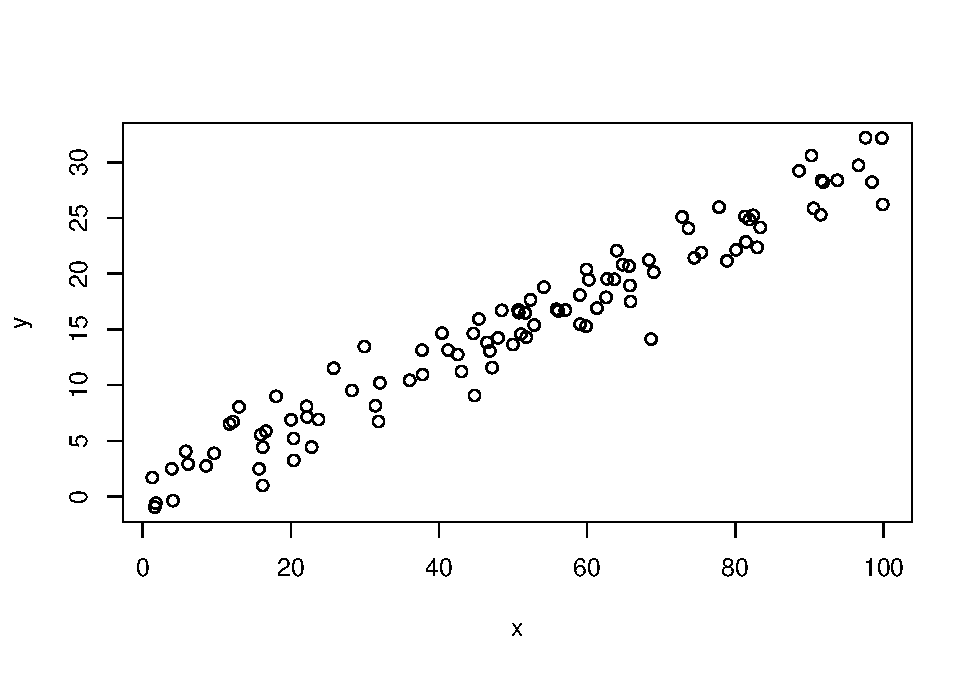
\includegraphics{R_ejercicios2021_files/figure-latex/unnamed-chunk-124-1.pdf}

\begin{Shaded}
\begin{Highlighting}[]
\NormalTok{modelo <-}\StringTok{ }\KeywordTok{lm}\NormalTok{(y }\OperatorTok{~}\StringTok{ }\NormalTok{x) }\CommentTok{# modelo lineal simple (distribución normal) de y en función de x }
\end{Highlighting}
\end{Shaded}

\begin{enumerate}
\def\labelenumi{\arabic{enumi}.}
\tightlist
\item
  ¿Qué tipo de objeto es modelo? Si la respuesta no es informativa recurrir a la ayuda de lm y leer la sección \textbf{value}
\end{enumerate}

2.¿Cuántos elementos tiene modelo?

\begin{enumerate}
\def\labelenumi{\arabic{enumi}.}
\setcounter{enumi}{2}
\tightlist
\item
  Utilizar los coeffientes del modelo (mediante indexación) para obtener el valor esperado de x= 3
\end{enumerate}

\begin{verbatim}
## (Intercept) 
##    1.377057
\end{verbatim}

\hypertarget{valores-esperados-lm-rrr}{%
\section{Valores esperados lm (RRR)}\label{valores-esperados-lm-rrr}}

\begin{enumerate}
\def\labelenumi{\arabic{enumi}.}
\tightlist
\item
  En base a los valores de los coeficientes (a, b) y utilizando la función \textbf{\emph{abline()}} agregar los valores esperados a la figura del punto anterior
\end{enumerate}

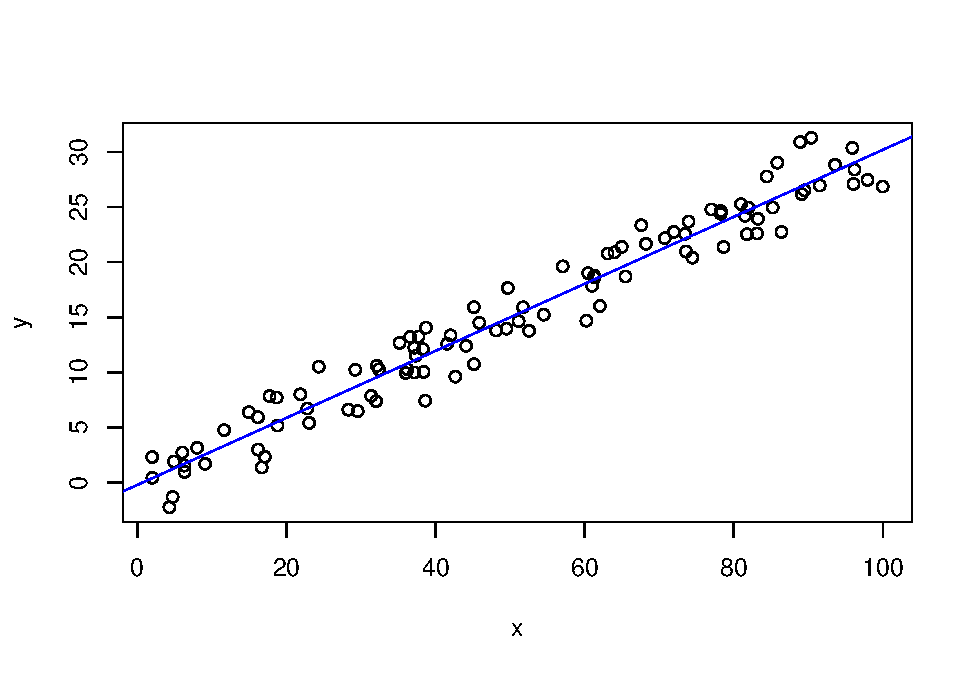
\includegraphics{R_ejercicios2021_files/figure-latex/unnamed-chunk-128-1.pdf}

\hypertarget{debugging-detectando-errores-4}{%
\section{Debugging, detectando errores}\label{debugging-detectando-errores-4}}

Correr las siguientes líneas de comando para generar datos de prueba. Examinar cada uno de los objetos

\begin{Shaded}
\begin{Highlighting}[]
\KeywordTok{rm}\NormalTok{( }\DataTypeTok{list =} \KeywordTok{ls}\NormalTok{() ) }\CommentTok{#eliminemos primero todos los objetos}
\end{Highlighting}
\end{Shaded}

\begin{Shaded}
\begin{Highlighting}[]
\NormalTok{  x <-}\StringTok{ }\KeywordTok{runif}\NormalTok{(}\DecValTok{100}\NormalTok{, }\DecValTok{10}\NormalTok{, }\DecValTok{100}\NormalTok{)}
\NormalTok{        y <-}\StringTok{ }\KeywordTok{rnorm}\NormalTok{(}\DecValTok{100}\NormalTok{, }\DecValTok{10}\NormalTok{ ,}\DecValTok{100}\NormalTok{)}
\NormalTok{        z <-}\StringTok{ }\KeywordTok{seq}\NormalTok{(}\DecValTok{0}\NormalTok{, }\DecValTok{200}\NormalTok{, }\DecValTok{2}\NormalTok{)}
\NormalTok{        g  <-}\StringTok{ }\KeywordTok{sample}\NormalTok{(letters, }\DecValTok{100}\NormalTok{, T)}

\NormalTok{        tabla <-}\StringTok{ }\KeywordTok{data.frame}\NormalTok{(x, y, g)}
\NormalTok{        matriz <-}\StringTok{ }\KeywordTok{matrix}\NormalTok{( }\KeywordTok{c}\NormalTok{(x, y, g ), }\DataTypeTok{ncol=}\DecValTok{3}\NormalTok{)}
\NormalTok{        lista <-}\StringTok{ }\KeywordTok{list}\NormalTok{(tabla, matriz)}
\end{Highlighting}
\end{Shaded}

Para cada una de las siguientes líneas de código explicar por que se obtiene un mensaje de error, warnning, o un resultado no esperado

\begin{enumerate}
\def\labelenumi{\arabic{enumi}.}
\item
\end{enumerate}

\begin{Shaded}
\begin{Highlighting}[]
\KeywordTok{dim}\NormalTok{( }\KeywordTok{data.frame}\NormalTok{(x, y, z) )}
\end{Highlighting}
\end{Shaded}

\begin{enumerate}
\def\labelenumi{\arabic{enumi}.}
\setcounter{enumi}{1}
\item
\end{enumerate}

\begin{Shaded}
\begin{Highlighting}[]
\KeywordTok{dim}\NormalTok{(X)}
\end{Highlighting}
\end{Shaded}

\begin{enumerate}
\def\labelenumi{\arabic{enumi}.}
\setcounter{enumi}{2}
\item
\end{enumerate}

\begin{Shaded}
\begin{Highlighting}[]
\KeywordTok{dim}\NormalTok{(y)}
\end{Highlighting}
\end{Shaded}

\begin{enumerate}
\def\labelenumi{\arabic{enumi}.}
\setcounter{enumi}{3}
\item
\end{enumerate}

\begin{Shaded}
\begin{Highlighting}[]
\KeywordTok{cbind}\NormalTok{(x, y, z)}
\end{Highlighting}
\end{Shaded}

\begin{enumerate}
\def\labelenumi{\arabic{enumi}.}
\setcounter{enumi}{4}
\item
\end{enumerate}

\begin{Shaded}
\begin{Highlighting}[]
\KeywordTok{matrix}\NormalTok{(}\DecValTok{1}\OperatorTok{:}\DecValTok{10}\NormalTok{, }\DataTypeTok{ncol=}\DecValTok{2}\NormalTok{, }\DataTypeTok{nrow=}\DecValTok{3}\NormalTok{)}
\end{Highlighting}
\end{Shaded}

\begin{enumerate}
\def\labelenumi{\arabic{enumi}.}
\setcounter{enumi}{6}
\item
\end{enumerate}

\begin{Shaded}
\begin{Highlighting}[]
\KeywordTok{matrix}\NormalTok{( }\KeywordTok{c}\NormalTok{(x, y, z), }\DataTypeTok{ncol=}\DecValTok{3}\NormalTok{ )}
\end{Highlighting}
\end{Shaded}

\begin{enumerate}
\def\labelenumi{\arabic{enumi}.}
\setcounter{enumi}{7}
\item
\end{enumerate}

\begin{Shaded}
\begin{Highlighting}[]
\NormalTok{matriz}\OperatorTok{$}\NormalTok{x}
\end{Highlighting}
\end{Shaded}

\begin{enumerate}
\def\labelenumi{\arabic{enumi}.}
\setcounter{enumi}{8}
\item
\end{enumerate}

\begin{Shaded}
\begin{Highlighting}[]
\KeywordTok{names}\NormalTok{( lista[}\DecValTok{1}\NormalTok{] )}
\end{Highlighting}
\end{Shaded}

\hypertarget{r09-gruxe1ficos-1}{%
\chapter*{R09 Gráficos 1}\label{r09-gruxe1ficos-1}}
\addcontentsline{toc}{chapter}{R09 Gráficos 1}

\hypertarget{figura-sencilla-r}{%
\section{Figura sencilla (R)}\label{figura-sencilla-r}}

Dados los siguientes objetos:

\begin{Shaded}
\begin{Highlighting}[]
\KeywordTok{set.seed}\NormalTok{(}\DecValTok{330}\NormalTok{)}
\NormalTok{x <-}\StringTok{ }\KeywordTok{runif}\NormalTok{(}\DecValTok{100}\NormalTok{)}
\KeywordTok{set.seed}\NormalTok{(}\DecValTok{100}\NormalTok{)}
\NormalTok{y <-}\StringTok{ }\DecValTok{3}\OperatorTok{*}\NormalTok{x }\OperatorTok{+}\StringTok{ }\KeywordTok{rnorm}\NormalTok{(}\DecValTok{100}\NormalTok{)}
\end{Highlighting}
\end{Shaded}

Obtener una figura como se muestra a continuación

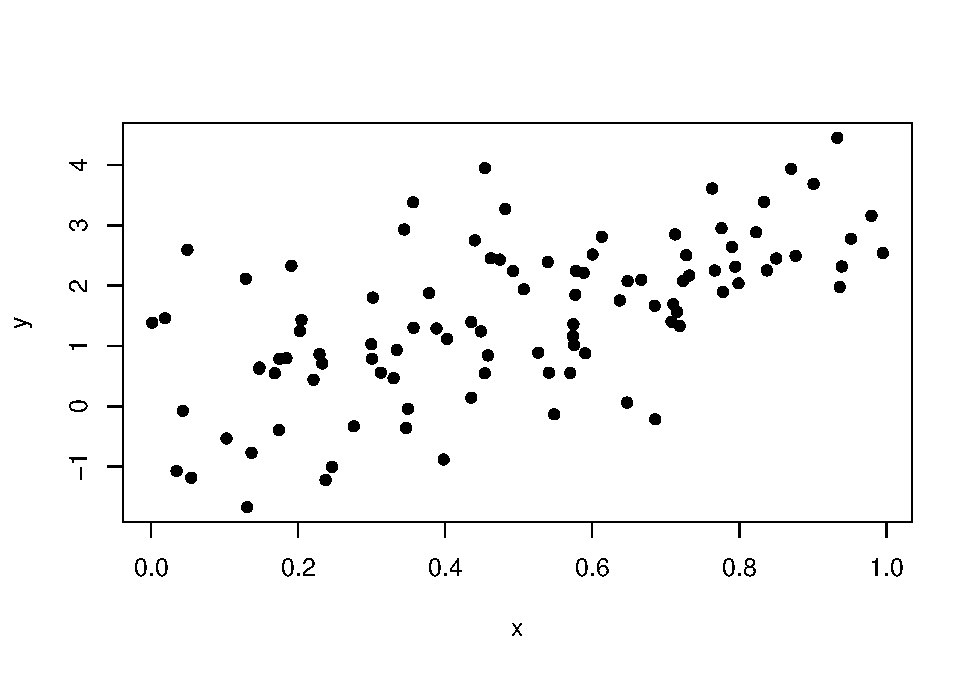
\includegraphics{R_ejercicios2021_files/figure-latex/unnamed-chunk-141-1.pdf}

\hypertarget{configurar-figuras-rr}{%
\section{Configurar figuras (RR)}\label{configurar-figuras-rr}}

Modificar la figura del punto anterior con las siguientes características

\begin{itemize}
\tightlist
\item
  El color de los puntos debe ser azul
\item
  La leyenda de los ejes \emph{y} y \emph{x} deberán decir respectivamente ``mi variable y'' y ``mi variable x''
\end{itemize}

\hypertarget{axis-rrr}{%
\section{axis (RRR)}\label{axis-rrr}}

Modificar el script para rotar la leyenda de los valores del eje y, de la figura anterior, como se muestra en la siguiente figura

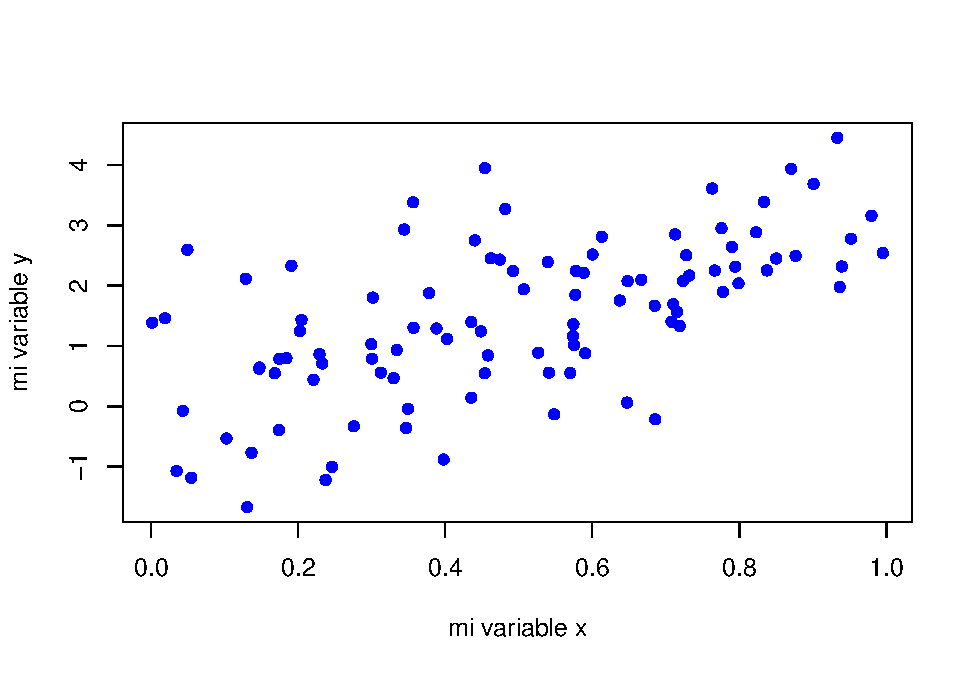
\includegraphics{R_ejercicios2021_files/figure-latex/unnamed-chunk-145-1.pdf}

Para hacerlo examinar las opciones del parámetro \textbf{\emph{las}}

\hypertarget{figura-sencilla-rr}{%
\section{Figura sencilla (RR)}\label{figura-sencilla-rr}}

\begin{enumerate}
\def\labelenumi{\arabic{enumi}.}
\tightlist
\item
  Importar el archivo DoubsEnv.csv que se encuentra en la carpeta 4-Datos (la descripción de la base de datos se encuentra en el archivo \url{datos_eer.html})
\end{enumerate}

\begin{verbatim}
  Site lon lat  das alt  pen  deb  pH dur  pho  nit  amm  oxy dbo   sec
1    1  88   7  0.3 934 48.0 0.84 7.9  45 0.01 0.20 0.00 12.2 2.7 upper
2    2  94  14  2.2 932  3.0 1.00 8.0  40 0.02 0.20 0.10 10.3 1.9 upper
3    3 102  18 10.2 914  3.7 1.80 8.3  52 0.05 0.22 0.05 10.5 3.5 upper
4    4 100  28 18.5 854  3.2 2.53 8.0  72 0.10 0.21 0.00 11.0 1.3 upper
5    5 106  39 21.5 849  2.3 2.64 8.1  84 0.38 0.52 0.20  8.0 6.2 upper
6    6 112  51 32.4 846  3.2 2.86 7.9  60 0.20 0.15 0.00 10.2 5.3 upper
\end{verbatim}

\begin{enumerate}
\def\labelenumi{\arabic{enumi}.}
\setcounter{enumi}{1}
\tightlist
\item
  Graficar mediante gráfico de dispersión (el default de plot) la relación entre las variables nit (x) y amm (y). Rotular los ejes x e y como se muestra en la figura
\end{enumerate}

\hypertarget{posiciones-doubs-rrr}{%
\section{Posiciones Doubs (RRR)}\label{posiciones-doubs-rrr}}

\begin{enumerate}
\def\labelenumi{\arabic{enumi}.}
\item
  Importar el archivo DoubsEnv.csv que se encuentra en la carpeta 4-Datos (la descripción de la base de datos se encuentra en el archivo \url{datos_eer.html})
\item
  Obtener la siguiente figura de las posiciones de los sitios de muestreo (Site, de la tabla DoubsEnv). Los colores negro, rojo y verde corresponden a las secciones (sec, de la tabla DoubsEnv) lower, middle y upper respectivamente.
\end{enumerate}

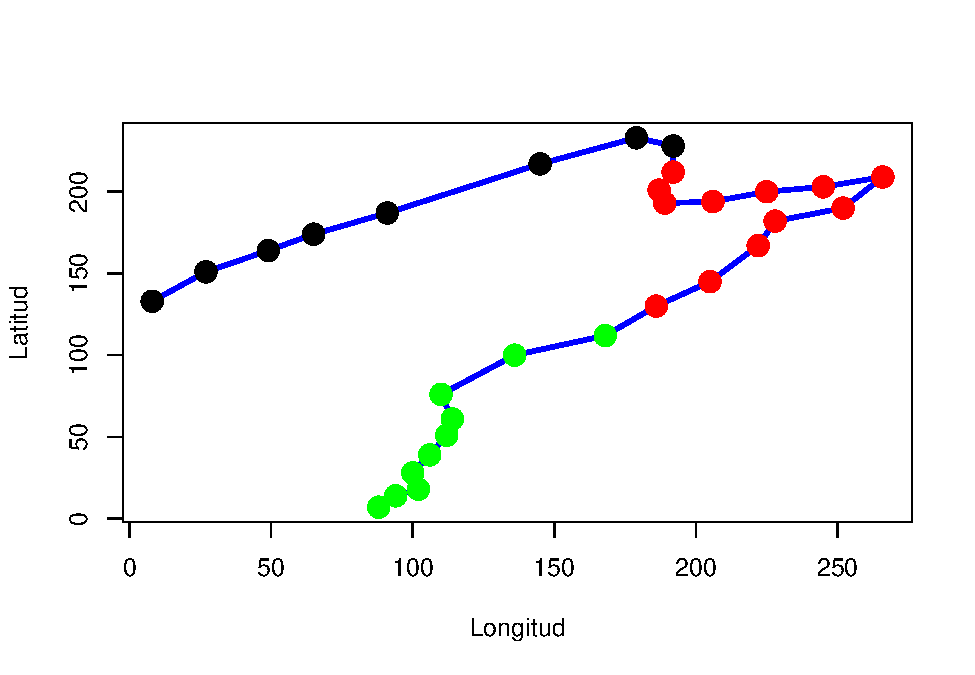
\includegraphics{R_ejercicios2021_files/figure-latex/unnamed-chunk-149-1.pdf}

Pasos sugeridos

\begin{itemize}
\tightlist
\item
  Generar una figura con toda la serie de datos (x= lon, y= lat), con lty= ``l'' (tipo de figura línea)
\item
  Generar tres objetos, cada uno con los registros correspondientes a las tres secciones del río (los objetos podrían llamares lower, middle y upper)
\item
  mediante points() agregar a la figura los puntos correspondientes a cada una de las secciones, utilizando los objetos recién generados
\end{itemize}

\hypertarget{rotulando-puntos-rrr}{%
\section{Rotulando puntos (RRR)}\label{rotulando-puntos-rrr}}

\begin{enumerate}
\def\labelenumi{\arabic{enumi}.}
\item
  Importar el archivo DoubsEnv.csv que se encuentra en la carpeta 4-Datos (la descripción de la base de datos se encuentra en el archivo \url{datos_eer.html})
\item
  Obtener la siguiente figura que corresponde a las posiciones de las estaciones de muestreo (variables lon y lat) y cuyo color corresponde a la sección (negro, rojo y verde para las secciones lower, middle y upper respectivamente). Donde cada número se refiere al ID del sitio (variable Site). Este paso puede hacerse mediante la función text(), donde los valores de \emph{\textbf{x}} y \emph{\textbf{y}} son los mismos usados en la figura
\end{enumerate}

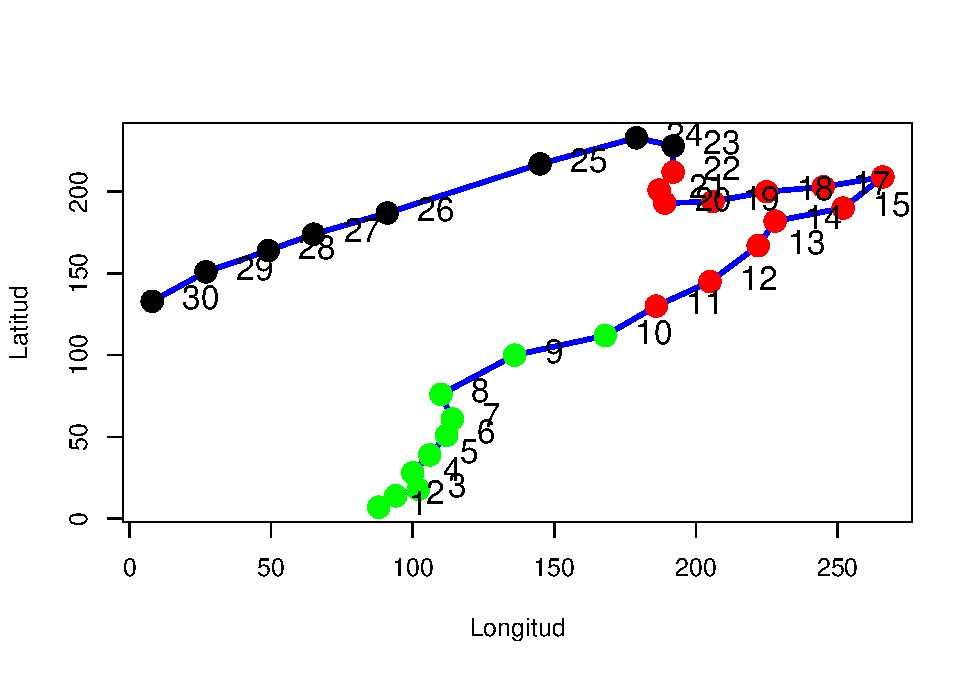
\includegraphics{R_ejercicios2021_files/figure-latex/unnamed-chunk-151-1.pdf}

\hypertarget{regresiuxf3n-rrrr}{%
\section{Regresión (RRRR)}\label{regresiuxf3n-rrrr}}

\begin{enumerate}
\def\labelenumi{\arabic{enumi}.}
\item
  Importar el archivo DoubsEnv.csv que se encuentra en la carpeta 4-Datos (la descripción de la base de datos se encuentra en el archivo \url{datos_eer.html})
\item
  Obtener la siguiente figura tomando las variables amm y pho como \emph{\textbf{y}} y \emph{\textbf{x}} respectivamente. Para agregar la línea de regresión utilizar la función \emph{\textbf{abline()}}, tomando los valores de pendiente e intercepto que se muestran en la figura. Los colores negro, rojo y verde corresponden a las secciones lower, middle y upper respectivamente.
\end{enumerate}

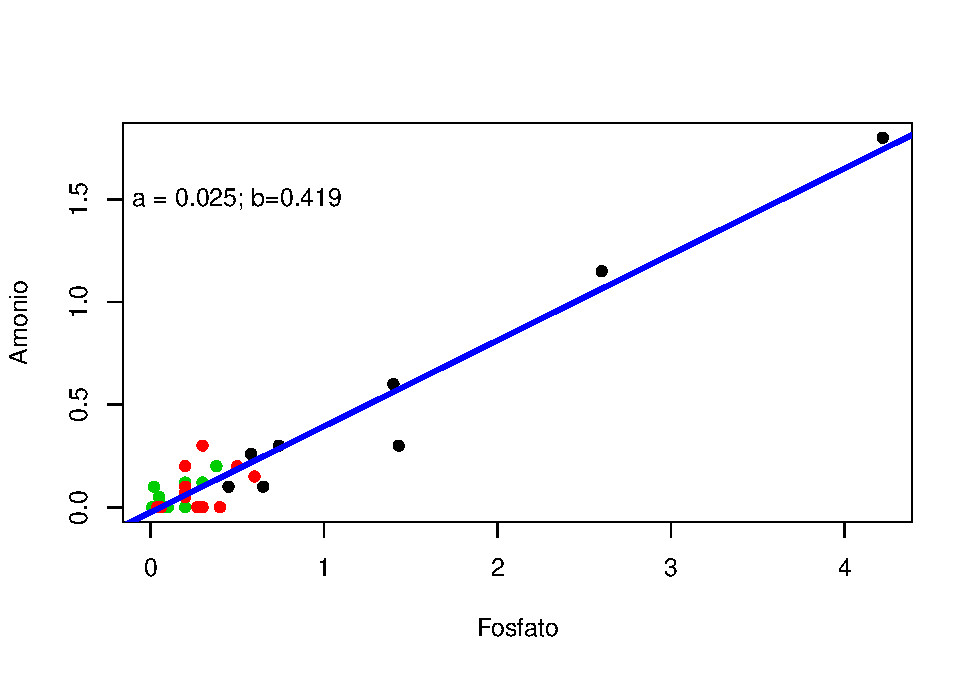
\includegraphics{R_ejercicios2021_files/figure-latex/unnamed-chunk-152-1.pdf}

\hypertarget{histograma-rrr}{%
\section{Histograma (RRR)}\label{histograma-rrr}}

\begin{enumerate}
\def\labelenumi{\arabic{enumi}.}
\tightlist
\item
  Importar el archivo DoubsEnv.csv que se encuentra en la carpeta 4-Datos (la descripción de la base de datos se encuentra en el archivo \url{datos_eer.html})
\end{enumerate}

Obtener la siguiente figura en base a la variable amm de DoubsEnv. Prestar atención a leyendas, tamaño de texto, colores y patrones de colores. Recurrir a la ayuda de hist()

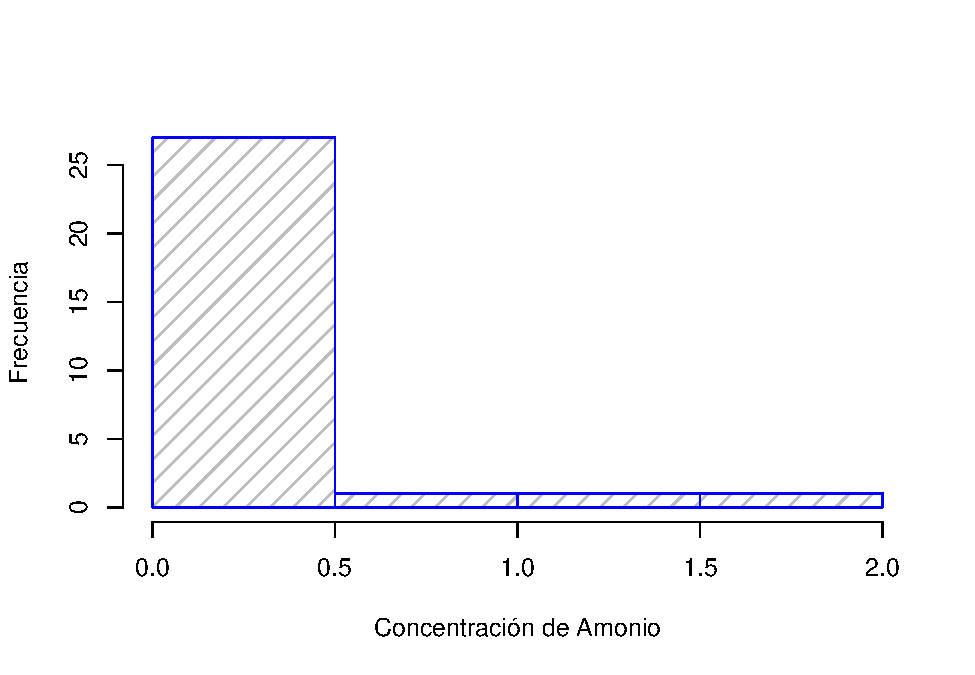
\includegraphics{R_ejercicios2021_files/figure-latex/unnamed-chunk-154-1.pdf}

\hypertarget{factores-para-ordenar-figuras-rrr}{%
\section{Factores para ordenar figuras (RRR)}\label{factores-para-ordenar-figuras-rrr}}

El archivo soil.RData contiene datos simulados de un experimento hipotético. En el experimento se tomaron valores de una variable hipotética (var) en cuatro sitios. En cada sitio se seleccionaron condiciones de suelo clasificadas en cuatro categorías en función de su calidad (fact).

\begin{enumerate}
\def\labelenumi{\arabic{enumi}.}
\item
  Explorar visualmente el objeto x. Utilizar str() para ver las características de sus variables
\item
  Se quiere realizar una figura como la que se muestra a continuación para evaluar si hay diferencias entre sitios y los tipos de suelo. ** NOTA ** Por ahora no nos vamos a preocupar por embellecer la figura, simplemente nos interesa que se muestre en el orden adecuado. Como se muestra a continuación
\end{enumerate}

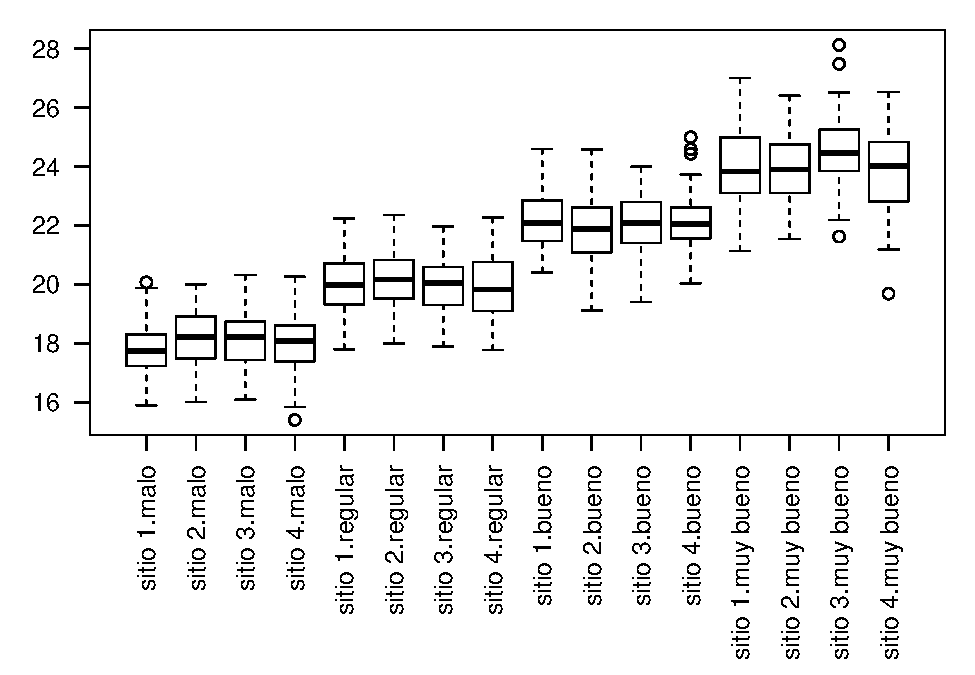
\includegraphics{R_ejercicios2021_files/figure-latex/unnamed-chunk-156-1.pdf}

Sin embargo boxplot() ordena a las variables por un índice alfabético, y por lo tanto con los datos recién generados la figura quedaría como se muestra a continuación (correr los siguientes comandos para confirmarlo).

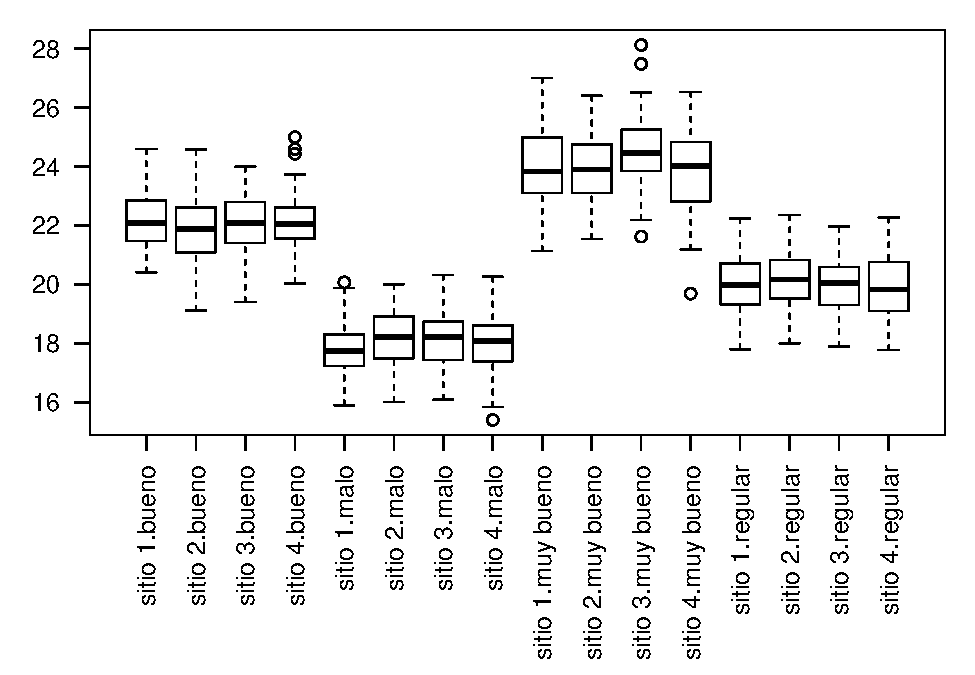
\includegraphics{R_ejercicios2021_files/figure-latex/unnamed-chunk-158-1.pdf}

Si bien los sitios aparecen ordenados nos gustaría que la figura también muestre los boxplot de la variable considerando el órden de las calidades de suelo (fact) como se muestra en la primera figura.

¿Cómo podríamos hacerlo? Este es uno de los casos donde los factores vienen a ayudarnos. La variable fact ya es un factor, pero éste no está ordenado!!! ** Ver la clase 07\_Objetos1.r la sección de factores **

\hypertarget{usando-reshape-para-generar-boxplots-rrr}{%
\section{Usando reshape para generar boxplots (RRR)}\label{usando-reshape-para-generar-boxplots-rrr}}

El objeto \emph{lago}, que se encuentra en el archivo \emph{4-Datos/lago.RData}, contiene datos de frecuencia relativa de presas en contenidos estomacales de truchas.

\begin{verbatim}
             ID year anfipodos  copepodos cladoceros ostracodos parabroteas
1 str01022017-2 2017  38.84514 52.7559055  3.6745407          0           0
2   str030217-2 2017  84.44976  0.9569378 10.0478469          0           0
3   str050207-1 2017  97.05015  0.2949853  0.1474926          0           0
4   str050217-2 2017  84.89583  4.6875000  6.7708333          0           0
5   str050217-3 2017  65.38462 28.8461538  5.7692308          0           0
6 str07022017-1 2017  84.07080  0.0000000  0.0000000          0           0
    larvas  insectos
1 0.000000  4.724409
2 0.000000  4.545455
3 0.000000  2.507375
4 1.041667  2.604167
5 0.000000  0.000000
6 0.000000 15.929204
\end{verbatim}

Se desea generar un gráfico boxplot mostrando variaciones en el contenido estomacal de truchas en tres años de muestreo, incluyendo solamente las tres presas más importantes en la dieta, como muestra la siguiente figura

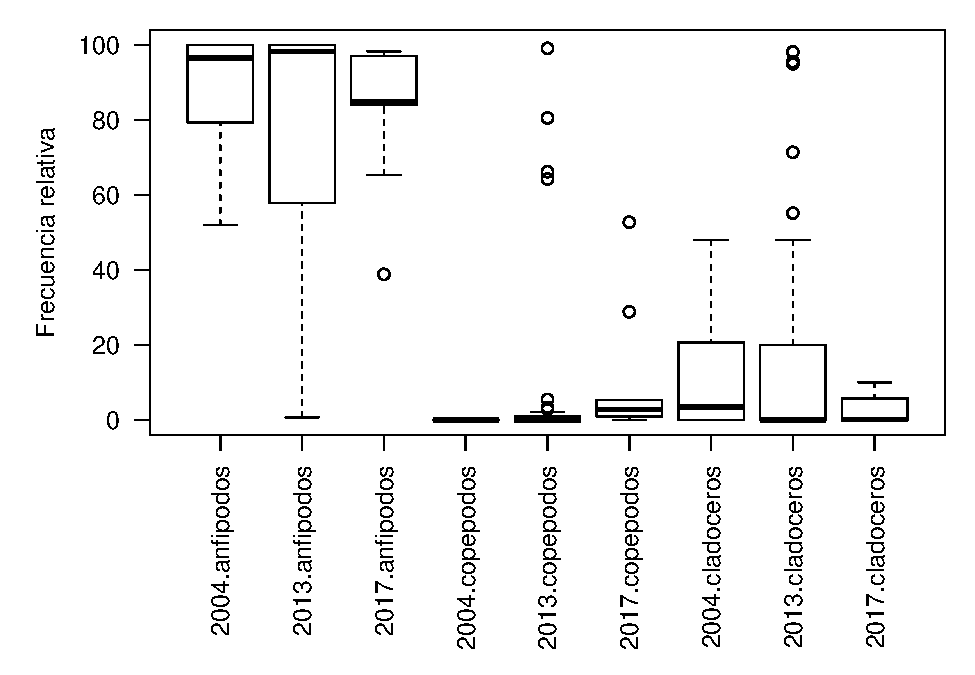
\includegraphics{R_ejercicios2021_files/figure-latex/unnamed-chunk-161-1.pdf}

Sin embargo, habrán notado que el objeto \emph{lago} está en formato ancho, mientras que la función boxplot requiere que los datos estén en formato largo

Seguir los siguientes pasos para generar la figura
1. Generar un nuevo objeto \emph{x} con las variables ``year'', ``anfipodos'',``copepodos'' y ``cladoceros''

\begin{enumerate}
\def\labelenumi{\arabic{enumi}.}
\setcounter{enumi}{1}
\tightlist
\item
  Usando la función adecuada del paquete \_reshape2, cambiar de formato ancho a formato largo y definir value.name= ``frec''
\end{enumerate}

\begin{Shaded}
\begin{Highlighting}[]
\KeywordTok{head}\NormalTok{(x); }\KeywordTok{tail}\NormalTok{(x)}
\end{Highlighting}
\end{Shaded}

\begin{verbatim}
##   year  variable     frec
## 1 2017 anfipodos 38.84514
## 2 2017 anfipodos 84.44976
## 3 2017 anfipodos 97.05015
## 4 2017 anfipodos 84.89583
## 5 2017 anfipodos 65.38462
## 6 2017 anfipodos 84.07080
\end{verbatim}

\begin{verbatim}
##     year   variable frec
## 193 2013 cladoceros    0
## 194 2013 cladoceros  NaN
## 195 2013 cladoceros  NaN
## 196 2013 cladoceros    0
## 197 2017 cladoceros    0
## 198 2017 cladoceros  NaN
\end{verbatim}

\begin{enumerate}
\def\labelenumi{\arabic{enumi}.}
\setcounter{enumi}{2}
\tightlist
\item
  Correr las siguientes líneas de comando para realizar la figura. NO es necesario endender cada uno de las líneas de comando utilizadas. La figura final tiene algunas modificaciones para lograr un formato más agradable. Si llamaron al objeto con otro nombre que no sea \emph{x}, cambiar únicamente las partes de boxplot donde se haga referencia al objeto \emph{x}
\end{enumerate}

\begin{Shaded}
\begin{Highlighting}[]
\NormalTok{ley <-}\StringTok{ }\KeywordTok{rep}\NormalTok{( }\KeywordTok{c}\NormalTok{(}\DecValTok{2004}\NormalTok{, }\DecValTok{2013}\NormalTok{, }\DecValTok{2017}\NormalTok{), }\DecValTok{3}\NormalTok{) }\CommentTok{## un vector con los nombres del eje x}
\ControlFlowTok{if}\NormalTok{ (}\KeywordTok{Sys.info}\NormalTok{()[}\StringTok{'sysname'}\NormalTok{] }\OperatorTok{==}\StringTok{ "Windows"}\NormalTok{) }\KeywordTok{windows}\NormalTok{() }\ControlFlowTok{else} \KeywordTok{x11}\NormalTok{() }\CommentTok{#chequea el sistema operativo (windows o linux) y abre una ventana gráfica de acuerdo a cada sistema}

\KeywordTok{par}\NormalTok{(}\DataTypeTok{mar=} \KeywordTok{c}\NormalTok{(}\DecValTok{6}\NormalTok{,}\DecValTok{5}\NormalTok{,}\DecValTok{1}\NormalTok{,}\DecValTok{1}\NormalTok{)) }\CommentTok{# define los valores de los márgenes de la figura}
\KeywordTok{boxplot}\NormalTok{(x}\OperatorTok{$}\NormalTok{frec }\OperatorTok{~}\StringTok{ }\NormalTok{x}\OperatorTok{$}\NormalTok{year }\OperatorTok{+}\StringTok{ }\NormalTok{x}\OperatorTok{$}\NormalTok{variable, }\DataTypeTok{names=}\NormalTok{ ley, }\DataTypeTok{las=} \DecValTok{2}\NormalTok{, }\DataTypeTok{ylab=} \StringTok{"Frecuencia relativa"}\NormalTok{, }\DataTypeTok{xlab=}\StringTok{""}\NormalTok{)}
  \KeywordTok{par}\NormalTok{(}\DataTypeTok{usr=} \KeywordTok{c}\NormalTok{(}\DecValTok{0}\NormalTok{, }\DecValTok{10}\NormalTok{, }\DecValTok{0}\NormalTok{, }\DecValTok{10}\NormalTok{) ) }\CommentTok{# redefine la escala de x e y de la figura}
  \KeywordTok{text}\NormalTok{(}\DataTypeTok{x=} \KeywordTok{c}\NormalTok{(}\FloatTok{1.5}\NormalTok{, }\FloatTok{3.8}\NormalTok{, }\DecValTok{6}\NormalTok{, }\FloatTok{8.5}\NormalTok{), }\DataTypeTok{y=} \DecValTok{-2}\NormalTok{, }\KeywordTok{c}\NormalTok{(}\StringTok{"anfipodos"}\NormalTok{,}\StringTok{"copepodos"}\NormalTok{, }\StringTok{"cladoceros"}\NormalTok{), }\DataTypeTok{xpd=} \OtherTok{NA}\NormalTok{) }\CommentTok{# el parámetro xpd= NA dice que text() opera fuera del área de trazado de la figura}
\end{Highlighting}
\end{Shaded}

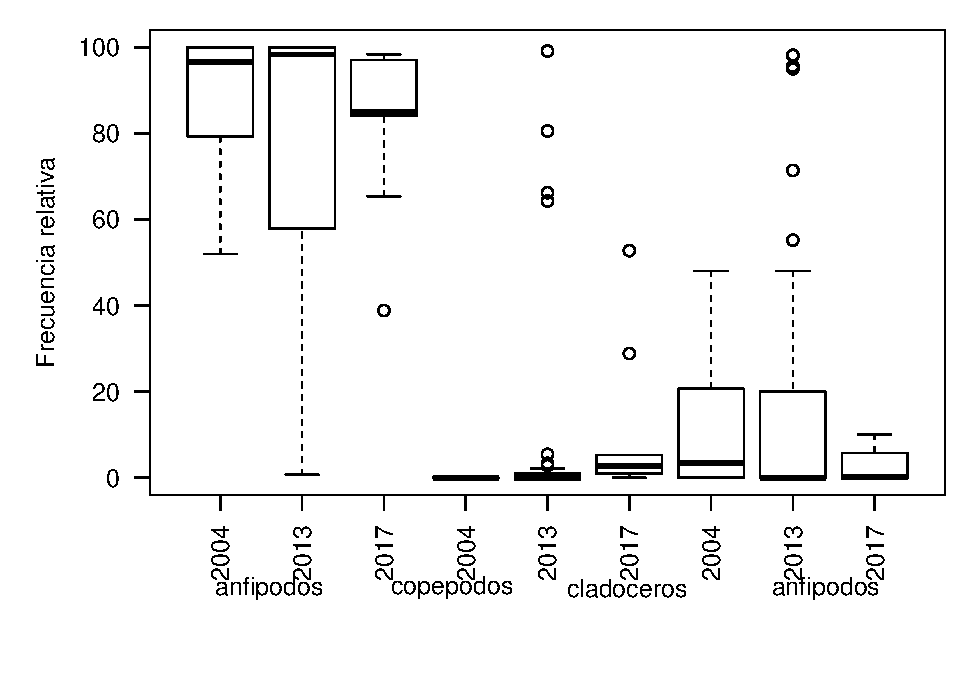
\includegraphics{R_ejercicios2021_files/figure-latex/unnamed-chunk-166-1.pdf}

\begin{Shaded}
\begin{Highlighting}[]
\KeywordTok{dev.off}\NormalTok{()}
\end{Highlighting}
\end{Shaded}

\begin{verbatim}
## pdf 
##   2
\end{verbatim}

\hypertarget{r10-gruxe1ficos-2}{%
\chapter*{R10 Gráficos 2}\label{r10-gruxe1ficos-2}}
\addcontentsline{toc}{chapter}{R10 Gráficos 2}

\hypertarget{figura-muxfaltiple-simple-rr}{%
\section{Figura múltiple simple (RR)}\label{figura-muxfaltiple-simple-rr}}

Trabajaremos con el objeto iris (del paquete base de R)

\begin{Shaded}
\begin{Highlighting}[]
\KeywordTok{head}\NormalTok{(iris)}
\end{Highlighting}
\end{Shaded}

\begin{verbatim}
##   Sepal.Length Sepal.Width Petal.Length Petal.Width Species
## 1          5.1         3.5          1.4         0.2  setosa
## 2          4.9         3.0          1.4         0.2  setosa
## 3          4.7         3.2          1.3         0.2  setosa
## 4          4.6         3.1          1.5         0.2  setosa
## 5          5.0         3.6          1.4         0.2  setosa
## 6          5.4         3.9          1.7         0.4  setosa
\end{verbatim}

Realizar una figura de dos paneles. En el panel superior graficar la relación entre las variables Sepal.Length y Sepal.With y en el panel inferior graficar un histograma de la variable Sepal.Length. En esta etapa no vamos a personalizar los ejes y leyendas, pero se espera que se modifiquen los parámetros \emph{\textbf{mar}} y \emph{\textbf{oma}} de \emph{\textbf{par()}}, para que la figura luzca similar a la que se muestra a continuación

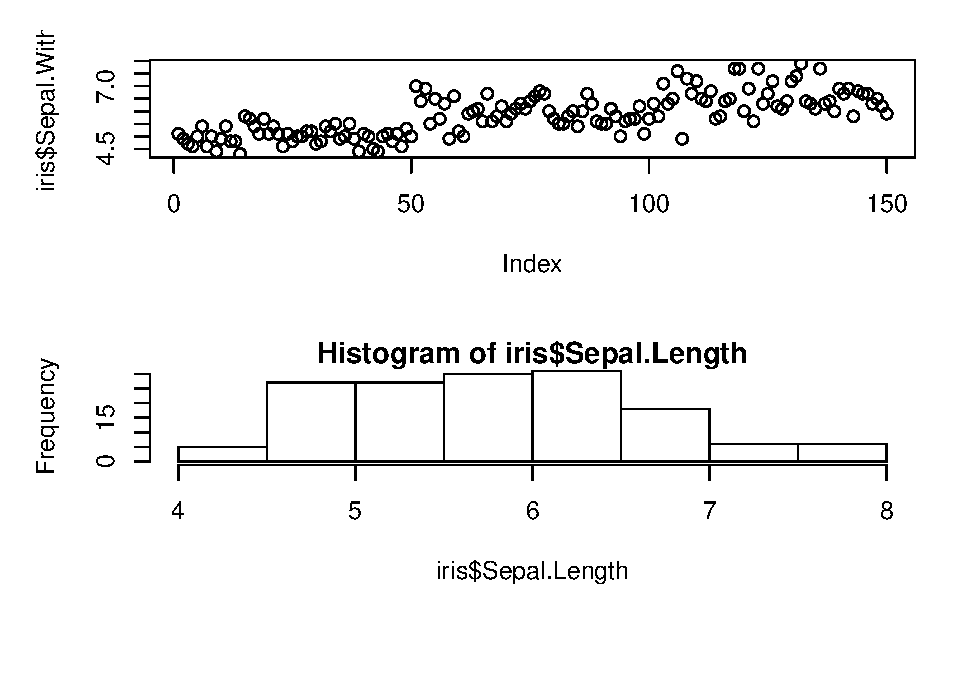
\includegraphics{R_ejercicios2021_files/figure-latex/unnamed-chunk-169-1.pdf}

\hypertarget{dispersiuxf3n-2-rr}{%
\section{Dispersión 2 (RR)}\label{dispersiuxf3n-2-rr}}

Dados los siguientes vectores (por ahora sólo importa el resultado y no como lo generamos)

Obtener la siguiente figura. Donde rojo corresponde a las hembras (H en el vector sexo) y azul a los machos (M en el vector sexo).\\
\textbf{Ayuda:} usar el vector sexo para indexar los vectores \textbf{\emph{x}} y \textbf{\emph{y}}.

\begin{Shaded}
\begin{Highlighting}[]
\NormalTok{x <-}\StringTok{ }\KeywordTok{runif}\NormalTok{(}\DecValTok{100}\NormalTok{, }\DecValTok{0}\NormalTok{, }\DecValTok{100}\NormalTok{)}
\NormalTok{y <-}\StringTok{ }\FloatTok{0.03} \OperatorTok{+}\StringTok{ }\DecValTok{3}\OperatorTok{*}\StringTok{ }\KeywordTok{rnorm}\NormalTok{(}\DecValTok{100}\NormalTok{, x, }\DecValTok{5}\NormalTok{)}
\NormalTok{yest <-}\StringTok{ }\FloatTok{0.03} \OperatorTok{+}\StringTok{ }\DecValTok{3}\OperatorTok{*}\NormalTok{x}
\NormalTok{sexo <-}\StringTok{ }\KeywordTok{rep}\NormalTok{(}\KeywordTok{c}\NormalTok{(}\StringTok{"H"}\NormalTok{, }\StringTok{"M"}\NormalTok{), }\DataTypeTok{each=}\DecValTok{50}\NormalTok{)}
\end{Highlighting}
\end{Shaded}

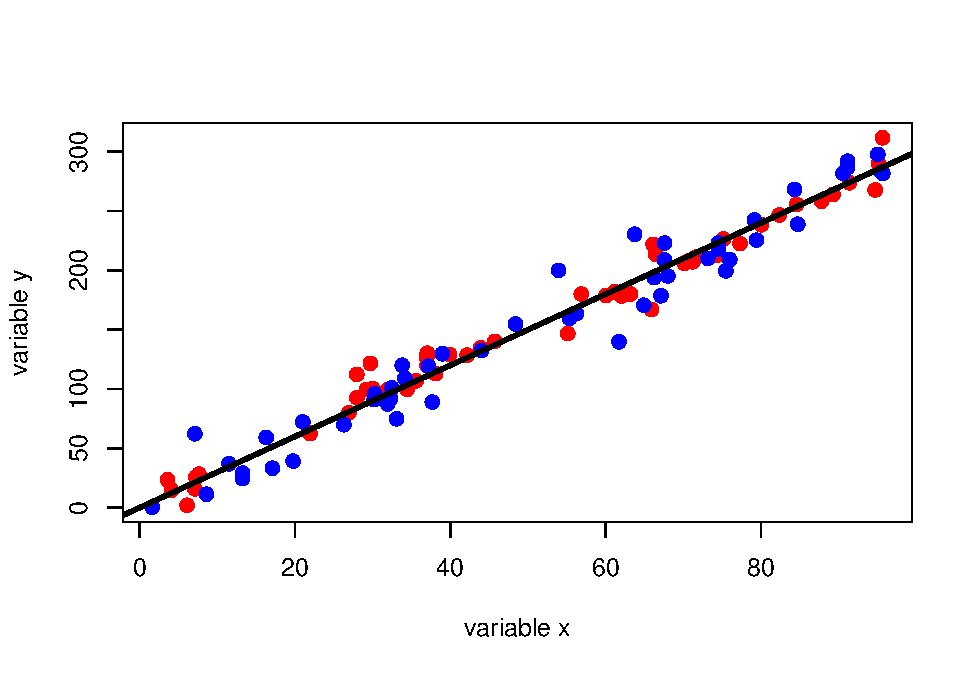
\includegraphics{R_ejercicios2021_files/figure-latex/unnamed-chunk-172-1.pdf}

1.2 Obtener la siguiente figura. Prestar atención a leyendas, espacios entre figuras, tamaño de símbolos y texto y colores

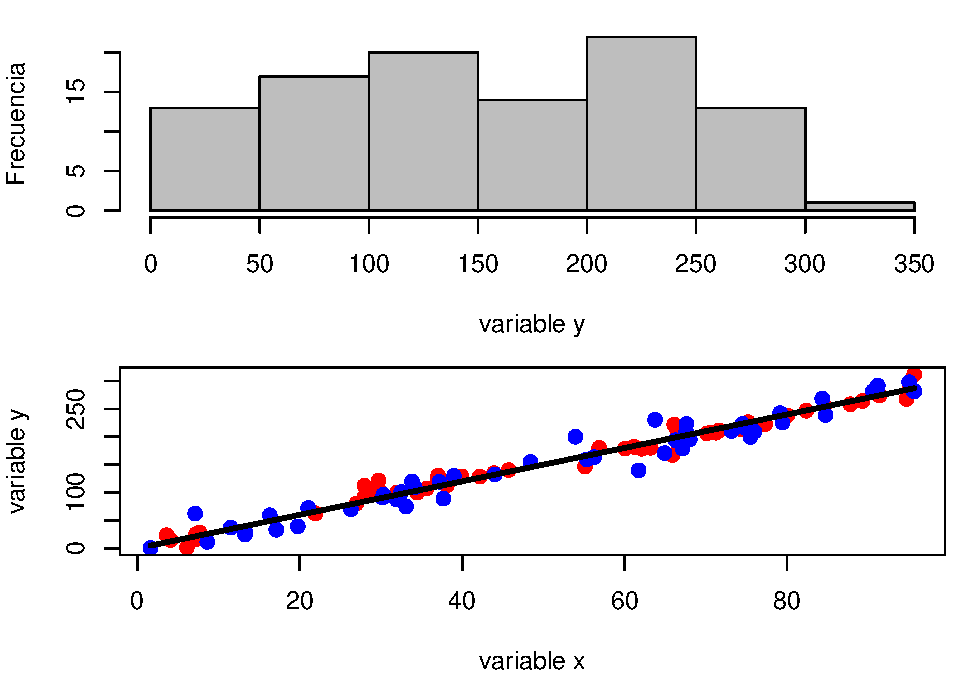
\includegraphics{R_ejercicios2021_files/figure-latex/unnamed-chunk-174-1.pdf}

\hypertarget{figura-completa-rrrr}{%
\section{Figura completa (RRRR)}\label{figura-completa-rrrr}}

\begin{enumerate}
\def\labelenumi{\arabic{enumi}.}
\item
  Importar el archivo DoubsEnv.csv que se encuentra en la carpeta 4-Datos (la descripción de la base de datos se encuentra en el archivo \url{datos_eer.html}).
\item
  Generar una figura múltiple de dos paneles, mostrando dos gráfico de dispersión. El gráfico del panel superior corresponde a la relación amonio (variable amm) vs fosfato (variable pho) y el del panel inferior a nitrato (ni) vs fosfato (pho). Los colores negro, rojo y verde corresponden respectivamente a las secciones lower, middle y upper.
\end{enumerate}

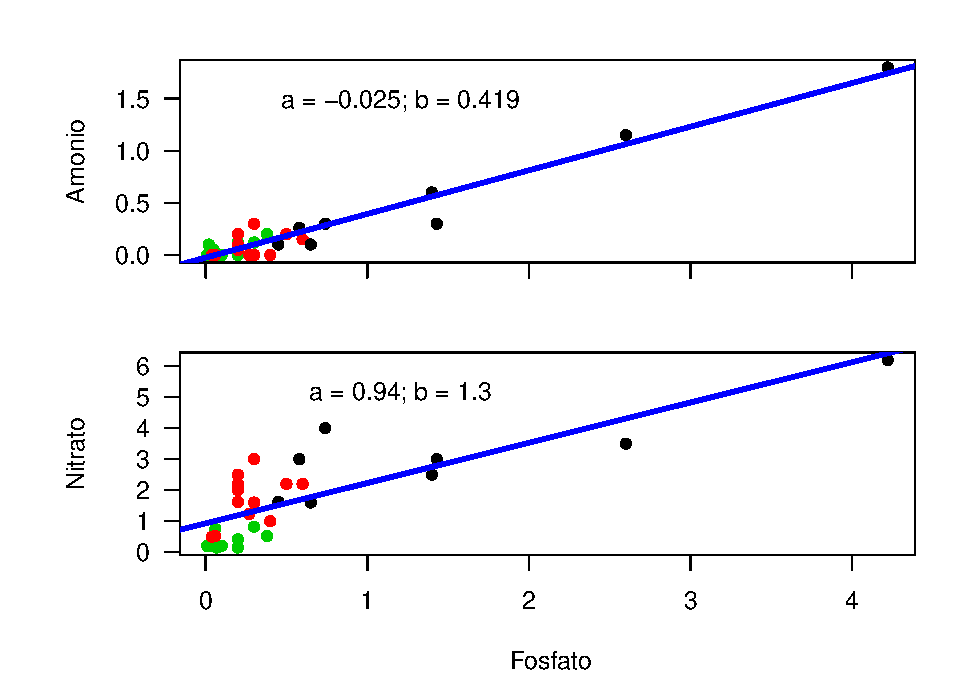
\includegraphics{R_ejercicios2021_files/figure-latex/unnamed-chunk-176-1.pdf}

Lineamientos generales

\begin{itemize}
\tightlist
\item
  Definir la función \emph{\textbf{par()}} para componer una figura con dos paneles (superior e inferior)\\
\item
  Generar la primera figura, que no debe tener rótulos en el eje x, para lo cual hay que especificar en \emph{\textbf{plot()}} que no queremos que lo grafique. Luego agregar un eje x mediante la funció \emph{\textbf{axis()}}
\item
  Utilizar la función \emph{\textbf{abline()}} para trazar la recta de regresión utilizando los valores que se muestran en la figura\\
\item
  Agregar la leyenda con los valores de los parámetros a y b mediante la función \emph{\textbf{text()}}. Considerar la conveniencia de definir el parámetro \emph{\textbf{usr}} dentro del \emph{\textbf{par()}} (ver archivo de clase)\\
\item
  Generar la segunda figura. Repetir los paso para la figura 1. En este caso el eje x tiene rótulos, pero queremos que la orientación de los rótulos de los ejes se muestren como en la figura de muestra. Por lo tanto, conviene volver a definir el eje utilizando \emph{\textbf{axis()}} como en la primera figura.\\
\item
  Utilizar los parámetros mar y oma para ajustar los márgenes internos y externos de la/las figuras
\end{itemize}

\begin{Shaded}
\begin{Highlighting}[]
\KeywordTok{par}\NormalTok{( }\DataTypeTok{mfrow=} \KeywordTok{c}\NormalTok{(), }\DataTypeTok{mar=}\KeywordTok{c}\NormalTok{(), }\DataTypeTok{oma=} \KeywordTok{c}\NormalTok{() )}
\KeywordTok{plot}\NormalTok{()}
\KeywordTok{axis}\NormalTok{()}
\KeywordTok{abline}\NormalTok{()}
\KeywordTok{par}\NormalTok{( }\DataTypeTok{usr=} \KeywordTok{c}\NormalTok{() )}
\KeywordTok{text}\NormalTok{()}
\CommentTok{#segunda figura}
\KeywordTok{plot}\NormalTok{()}
\KeywordTok{axis}\NormalTok{()}
\KeywordTok{abline}\NormalTok{()}
\KeywordTok{par}\NormalTok{( }\DataTypeTok{usr=} \KeywordTok{c}\NormalTok{() )}
\KeywordTok{text}\NormalTok{()}
\end{Highlighting}
\end{Shaded}

\hypertarget{r11-gruxe1ficos3}{%
\chapter*{R11 Gráficos3}\label{r11-gruxe1ficos3}}
\addcontentsline{toc}{chapter}{R11 Gráficos3}

\hypertarget{pairs-rr}{%
\section{Pairs (RR)}\label{pairs-rr}}

\begin{enumerate}
\def\labelenumi{\arabic{enumi}.}
\item
  Asignar a un objeto que llamaremos \textbf{\emph{env}} la tabla contenida en el archivo DoubsEnv.csv que se encuentra en la carpeta 4-Datos (la descripción de la base de datos se encuentra en el archivo \url{datos_eer.html}).
\item
  Utilizar la función \emph{pairs()} para analizar la relación entre las variables correspondientes a las columnas 7 a 14 de \textbf{\emph{env}}.
\end{enumerate}

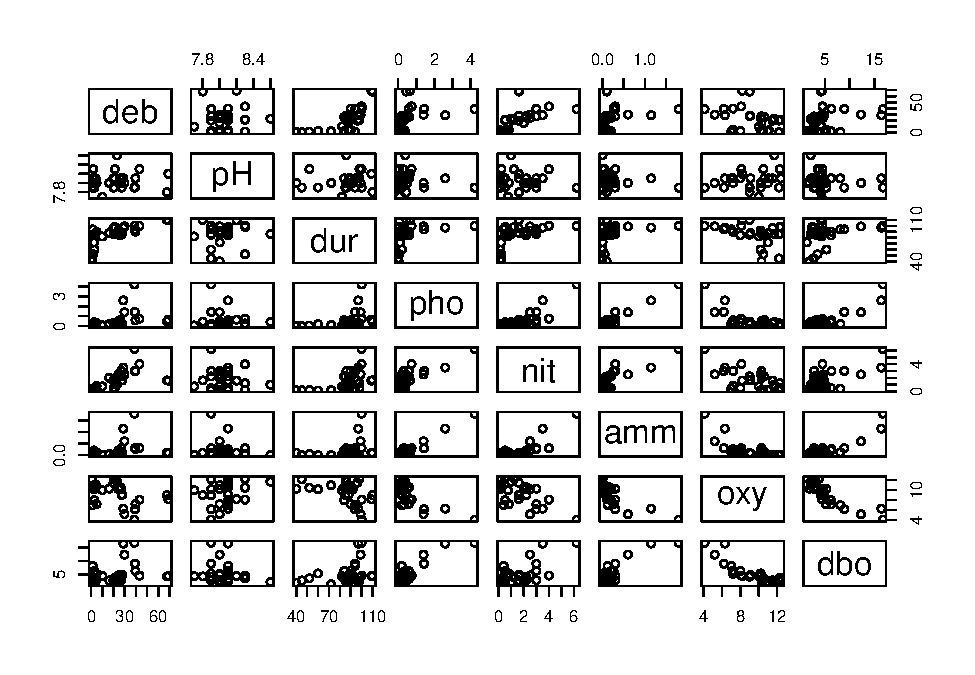
\includegraphics{R_ejercicios2021_files/figure-latex/unnamed-chunk-179-1.pdf}

\hypertarget{boxplot}{%
\section{Boxplot}\label{boxplot}}

Generar una figura boxplot de la variable fosfato (pho) discriminando por sección del río Doubs. Notar la orientación de la leyenda de los ejes. Recurrir a la función \emph{\textbf{axis()}}.

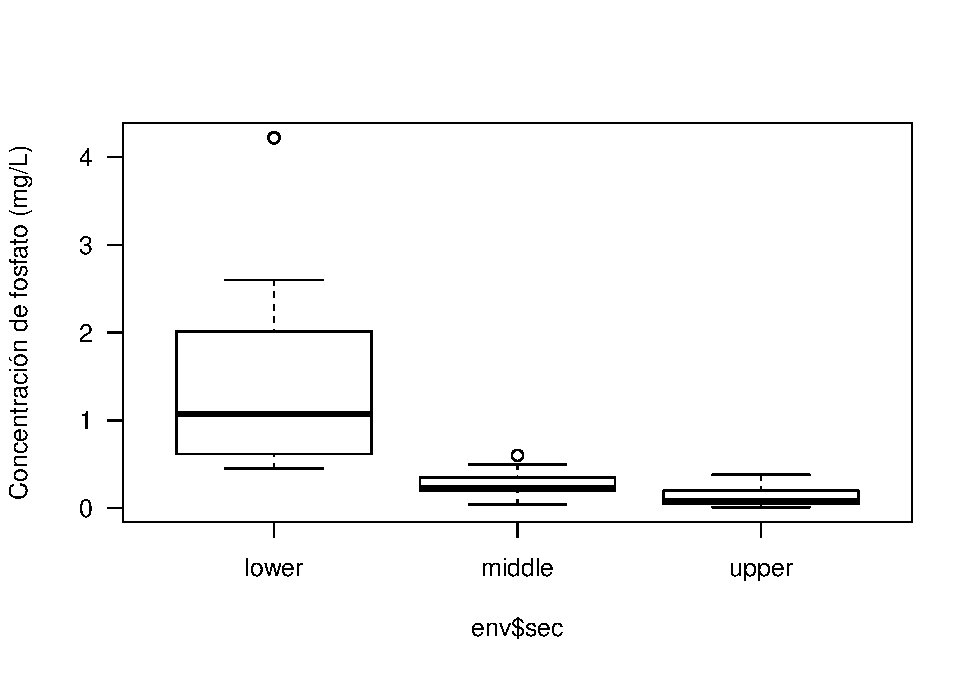
\includegraphics{R_ejercicios2021_files/figure-latex/unnamed-chunk-181-1.pdf}

\hypertarget{gruxe1ficos-condicionales-xyplot}{%
\section{Gráficos condicionales xyplot}\label{gruxe1ficos-condicionales-xyplot}}

Utilizando las función gráfica \emph{\textbf{xyplot()}} del paquete \emph{\textbf{lattice}} generar una figura múltiple como la mostrada a continuación

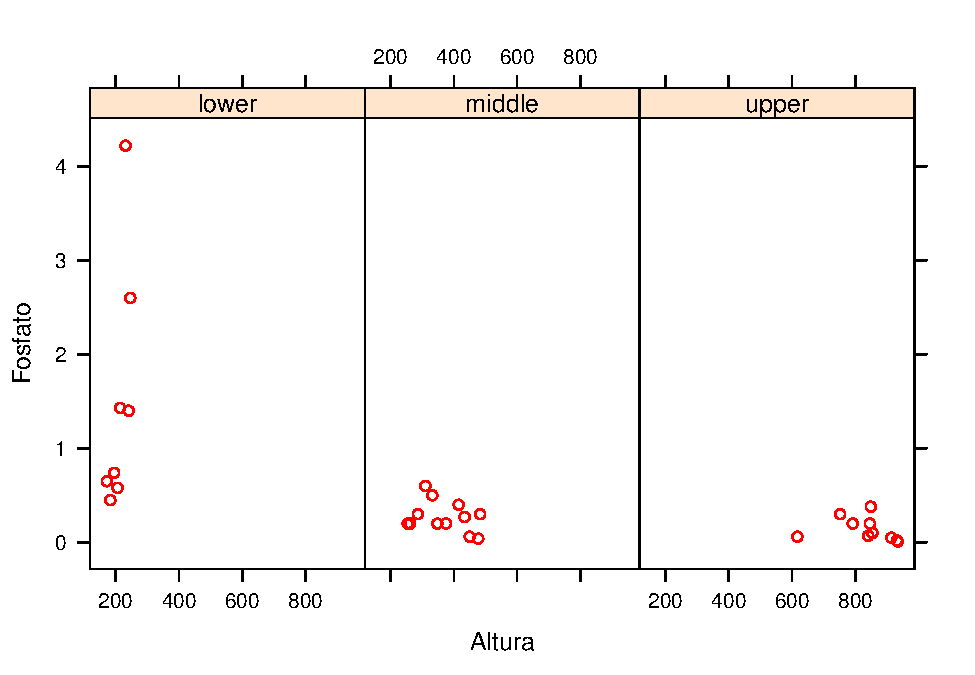
\includegraphics{R_ejercicios2021_files/figure-latex/unnamed-chunk-183-1.pdf}

\begin{verbatim}
## X11cairo 
##        3
\end{verbatim}

La figura muestra la relación entre las variables fosfato (pho) y altura (alt) condicional a las tres secciones del río

\hypertarget{gruxe1ficos-condicionales-coplot}{%
\section{Gráficos condicionales coplot}\label{gruxe1ficos-condicionales-coplot}}

Utilizar la función coplot del paquete lattice para generar la siguiente figura

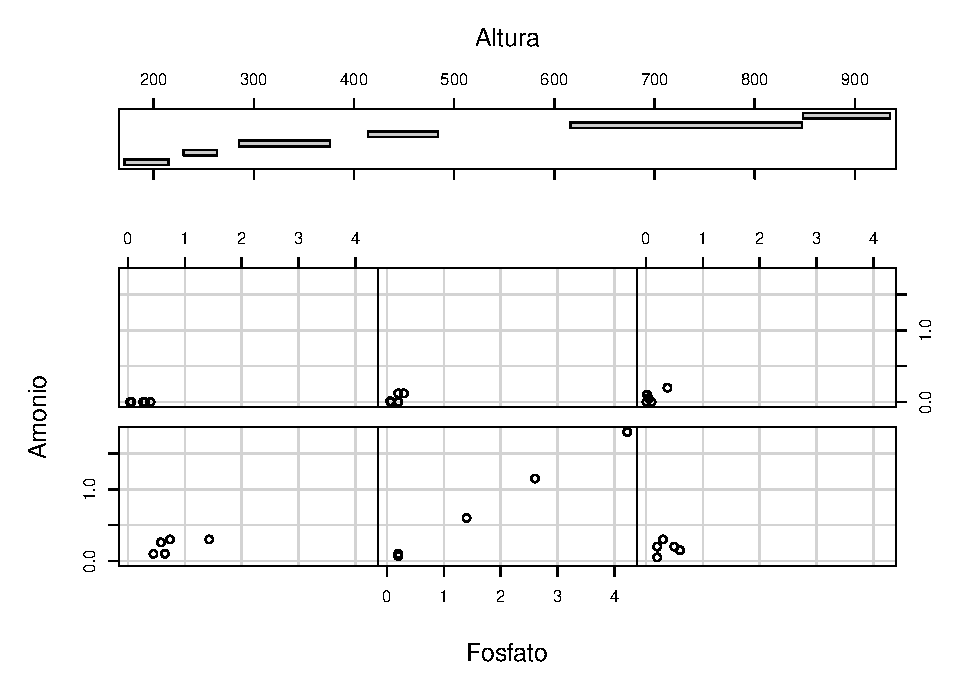
\includegraphics{R_ejercicios2021_files/figure-latex/unnamed-chunk-185-1.pdf}

\begin{verbatim}
## pdf 
##   2
\end{verbatim}

La figura muestra la relación entre las variables amonio (amm) y fosfato (pho) condicional a rangos de valores de altura (alt), con parámetro de \_\textbf{overlap= 0.1.\\
}NOTA** el argumento xlab es un vector con dos elementos para los ejes x inferior (primer elemento) y superior (segundo elemento). Entonces definir xlab= c(``Fosfato'', ``Altura'').

\hypertarget{debugging-detectando-errores-5}{%
\section{Debugging, detectando errores}\label{debugging-detectando-errores-5}}

Correr las siguientes líneas de comando para generar datos de prueba. Examinar cada uno de los objetos

\begin{Shaded}
\begin{Highlighting}[]
\KeywordTok{rm}\NormalTok{( }\DataTypeTok{list =} \KeywordTok{ls}\NormalTok{() ) }\CommentTok{#eliminemos primero todos los objetos}
\end{Highlighting}
\end{Shaded}

\begin{Shaded}
\begin{Highlighting}[]
\NormalTok{    x <-}\StringTok{ }\KeywordTok{runif}\NormalTok{(}\DecValTok{100}\NormalTok{,}\DecValTok{10}\NormalTok{, }\DecValTok{100}\NormalTok{)}
\NormalTok{    y <-}\StringTok{ }\KeywordTok{rnorm}\NormalTok{(}\DecValTok{100}\NormalTok{, }\DecValTok{10}\NormalTok{ ,}\DecValTok{100}\NormalTok{)}
\NormalTok{    z <-}\StringTok{ }\KeywordTok{seq}\NormalTok{(}\DecValTok{0}\NormalTok{,}\DecValTok{200}\NormalTok{, }\DecValTok{2}\NormalTok{)}
\NormalTok{        g  <-}\StringTok{ }\KeywordTok{sample}\NormalTok{(letters,}\DecValTok{100}\NormalTok{, T)}

\NormalTok{        tabla <-}\StringTok{ }\KeywordTok{data.frame}\NormalTok{(x,y,g)}
\NormalTok{        matriz <-}\StringTok{ }\KeywordTok{matrix}\NormalTok{(}\KeywordTok{c}\NormalTok{(x,y,g), }\DataTypeTok{ncol=}\DecValTok{3}\NormalTok{)}
\NormalTok{        lista <-}\StringTok{ }\KeywordTok{list}\NormalTok{(tabla, matriz)}
\end{Highlighting}
\end{Shaded}

Para cada una de las siguientes líneas de código explicar por que se obtiene un mensaje de error, warnning, o un resultado no esperado

\begin{enumerate}
\def\labelenumi{\arabic{enumi}.}
\item
\end{enumerate}

\begin{Shaded}
\begin{Highlighting}[]
\KeywordTok{plot}\NormalTok{(x,y, }\DataTypeTok{pch =} \DecValTok{16}\NormalTok{, }\DataTypeTok{col =}\NormalTok{ blue)}
\end{Highlighting}
\end{Shaded}

\begin{enumerate}
\def\labelenumi{\arabic{enumi}.}
\setcounter{enumi}{1}
\item
\end{enumerate}

\begin{Shaded}
\begin{Highlighting}[]
\NormalTok{mhist <-}\StringTok{ }\KeywordTok{hist}\NormalTok{(x)}\ErrorTok{)}
\end{Highlighting}
\end{Shaded}

\begin{enumerate}
\def\labelenumi{\arabic{enumi}.}
\setcounter{enumi}{2}
\item
\end{enumerate}

\begin{Shaded}
\begin{Highlighting}[]
\KeywordTok{plot}\NormalTok{(x, y, }\DataTypeTok{pch =} \DecValTok{16}\NormalTok{, }\DataTypeTok{label =}\NormalTok{ T, }\DataTypeTok{col =} \StringTok{"orange"}\NormalTok{, }\DataTypeTok{main=}\StringTok{"mifigura"}\NormalTok{)}
\end{Highlighting}
\end{Shaded}

\begin{enumerate}
\def\labelenumi{\arabic{enumi}.}
\setcounter{enumi}{3}
\item
\end{enumerate}

\begin{Shaded}
\begin{Highlighting}[]
\KeywordTok{plot}\NormalTok{(x, y, }\KeywordTok{ylim}\NormalTok{(}\DecValTok{1}\NormalTok{,}\DecValTok{100}\NormalTok{))}
\end{Highlighting}
\end{Shaded}

\begin{enumerate}
\def\labelenumi{\arabic{enumi}.}
\setcounter{enumi}{4}
\item
\end{enumerate}

\begin{Shaded}
\begin{Highlighting}[]
\KeywordTok{barplot}\NormalTok{(g)}
\end{Highlighting}
\end{Shaded}

\begin{enumerate}
\def\labelenumi{\arabic{enumi}.}
\setcounter{enumi}{5}
\item
\end{enumerate}

\begin{Shaded}
\begin{Highlighting}[]
\KeywordTok{plot}\NormalTok{(x, y, }\DataTypeTok{col=}\KeywordTok{c}\NormalTok{(}\StringTok{"red"}\NormalTok{, }\StringTok{"green"} \StringTok{"blue"}\NormalTok{))}
\end{Highlighting}
\end{Shaded}

\begin{enumerate}
\def\labelenumi{\arabic{enumi}.}
\setcounter{enumi}{6}
\item
\end{enumerate}

\begin{Shaded}
\begin{Highlighting}[]
\KeywordTok{plot}\NormalTok{(x, y, }\DataTypeTok{pch =} \DecValTok{16}\NormalTok{, }\DataTypeTok{col =} \StringTok{"orange"}\NormalTok{, }\DataTypeTok{main=}\StringTok{""")}
\end{Highlighting}
\end{Shaded}

\hypertarget{r12-resumir}{%
\chapter*{R12 Resumir}\label{r12-resumir}}
\addcontentsline{toc}{chapter}{R12 Resumir}

\hypertarget{summary-r}{%
\section{summary (R)}\label{summary-r}}

Asignar a un objeto que llamaremos \textbf{\emph{env}} la tabla contenida en el archivos DoubsEnv.csv, que se encuentra en la carpeta 4-Datos (la descripción de la base de datos se encuentra en el archivo \url{datos_eer.html}).

Asignar la salida de la función \textbf{\emph{summary(env)}} a un objeto que llamaremos \textbf{\emph{resumen}}
* ¿Qué clase de objeto es \textbf{\emph{resumen}}?

\hypertarget{table-r}{%
\section{table (R)}\label{table-r}}

Aplicar la función \textbf{\emph{table()}} a la variable sec
¿qué información nos da esta salida?

\hypertarget{apply-rr}{%
\section{apply (RR)}\label{apply-rr}}

\begin{enumerate}
\def\labelenumi{\arabic{enumi}.}
\item
  Asignar a un objeto que llamaremos \textbf{\emph{env}} la tabla contenida en el archivos DoubsEnv.csv que se encuentra en la carpeta 4-Datos (la descripción de la base de datos se encuentra en el archivo \url{datos_eer.html}).
\item
  Utilizando la función apply() calcular el rango de valores de cada una de las variables de campo de env (variables 4 a 14)
\end{enumerate}

\hypertarget{apply-rrr}{%
\section{apply (RRR)}\label{apply-rrr}}

\begin{enumerate}
\def\labelenumi{\arabic{enumi}.}
\item
  Asignar a un objeto que llamaremos \textbf{\emph{env}} la tabla contenida en el archivos DoubsEnv.csv que se encuentra en la carpeta 4-Datos (la descripción de la base de datos se encuentra en el archivo \url{datos_eer.html}).
\item
  Utilizando la función \textbf{\emph{apply()}} generar una figura múltiple de 8 paneles (4 filas y dos columnas) utilizando las columnas 7 a 14 de env. La figura se muestra a continuación
\end{enumerate}

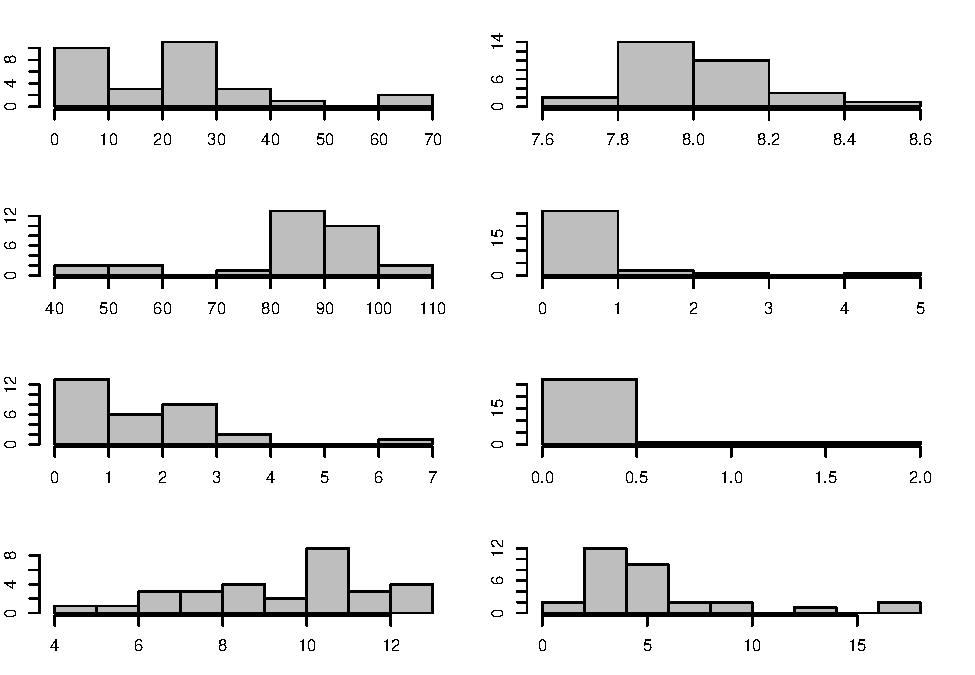
\includegraphics{R_ejercicios2021_files/figure-latex/unnamed-chunk-200-1.pdf}

Estructura

\begin{Shaded}
\begin{Highlighting}[]
\KeywordTok{par}\NormalTok{(}\DataTypeTok{mfrow=}\KeywordTok{c}\NormalTok{(}\DecValTok{4}\NormalTok{,}\DecValTok{2}\NormalTok{), }\DataTypeTok{mar=} \KeywordTok{c}\NormalTok{(}\DecValTok{3}\NormalTok{,}\DecValTok{2}\NormalTok{,}\DecValTok{2}\NormalTok{,}\DecValTok{2}\NormalTok{))}
\KeywordTok{apply}\NormalTok{(COMPLETAR)}
\end{Highlighting}
\end{Shaded}

\hypertarget{tapply-rrr}{%
\section{tapply (RRR)}\label{tapply-rrr}}

Asignar a un objeto que llamaremos \textbf{\emph{env}} la tabla contenida en el archivos DoubsEnv.csv que se encuentra en la carpeta 4-Datos (la descripción de la base de datos se encuentra en el archivo \url{datos_eer.html}).

Utilizar la función tapply para estimar los cuantiles 5 y 95 de la variable pho del objeto \textbf{\emph{env}} categorizando por sección del río (sec). Asignar la salida a un objeto que llamaremos \textbf{\emph{tabla}}. La función para necesaria es quantile (recurrir a la ayuda)

\begin{itemize}
\tightlist
\item
  ¿Qué clase de objeto es \textbf{\emph{tabla}} ?
\end{itemize}

\hypertarget{muxfaltiples-variables-rr}{%
\section{Múltiples variables (RR)}\label{muxfaltiples-variables-rr}}

\begin{enumerate}
\def\labelenumi{\arabic{enumi}.}
\tightlist
\item
  Utilizar una función de la que hemos visto en la clase R12\_Resumir para calcular el valor de la mediana de las variables ambientales del objeto \textbf{\emph{env}} para cada una de las secciones del río
\end{enumerate}

\hypertarget{grep-which-resumir-rrrr}{%
\section{grep() which() resumir (RRRR)}\label{grep-which-resumir-rrrr}}

El archivo ``SP\_aves\_BI.csv'', de la carpeta 4-Datos, contiene un listado de aves de Sudamérica categorizadas de acuerdo a su estado de conservación ( \href{http://www.birdlife.org/datazone/}{BirdLife International}
Las especies fueron clasificadas en las siguientes categorías:

Threatened Species

CR - Critically Endangered

CR (PE) - Critically Endangered (Possibly Extinct)

CR (PEW) - Critically Endangered (Possibly Extinct In The Wild)

EN - Endangered

VU - Vulnerable

NT - Near Threatened

LC - Least Concern

DD - Data Deficient

Responder los siguientes puntos\\
1. ¿cuántas especies hay listadas en cada una de las categorías de amenaza?\\
2. ¿cuántas especies de cada género se encuentran en cada una de las categorías de amenaza?\\
3. ¿cuál es el género con mayor número de especies listadas?\\
4. Identificar las especies del género \emph{Larus} (gaviotas) que se encuentren en las categorías NT (Near threatened) o VU (vulnerable).

\hypertarget{debugging-detectando-errores-6}{%
\section{Debugging, detectando errores}\label{debugging-detectando-errores-6}}

Correr las siguientes líneas de comando para generar datos de prueba. Examinar cada uno de los objetos

\begin{Shaded}
\begin{Highlighting}[]
\KeywordTok{rm}\NormalTok{( }\DataTypeTok{list =} \KeywordTok{ls}\NormalTok{() ) }\CommentTok{#eliminemos primero todos los objetos}
\end{Highlighting}
\end{Shaded}

\begin{Shaded}
\begin{Highlighting}[]
\NormalTok{x <-}\StringTok{ }\KeywordTok{runif}\NormalTok{(}\DecValTok{100}\NormalTok{,}\DecValTok{10}\NormalTok{, }\DecValTok{100}\NormalTok{)}
\NormalTok{y <-}\StringTok{ }\KeywordTok{rnorm}\NormalTok{(}\DecValTok{100}\NormalTok{, }\DecValTok{10}\NormalTok{ ,}\DecValTok{100}\NormalTok{)}
\NormalTok{z <-}\StringTok{ }\KeywordTok{seq}\NormalTok{(}\DecValTok{0}\NormalTok{,}\DecValTok{200}\NormalTok{, }\DecValTok{2}\NormalTok{)}
\NormalTok{g  <-}\StringTok{ }\KeywordTok{sample}\NormalTok{(letters,}\DecValTok{100}\NormalTok{,T)}

\NormalTok{tabla <-}\StringTok{ }\KeywordTok{data.frame}\NormalTok{(x,y,g)}
\NormalTok{matriz <-}\StringTok{ }\KeywordTok{matrix}\NormalTok{(}\KeywordTok{c}\NormalTok{(x,y,g), }\DataTypeTok{ncol=}\DecValTok{3}\NormalTok{)}
\NormalTok{lista <-}\StringTok{ }\KeywordTok{list}\NormalTok{(tabla, matriz)}
\end{Highlighting}
\end{Shaded}

Para cada una de las siguientes líneas de código explicar porqué se obtiene un mensaje de error, warnning, o un resultado no esperado

\begin{enumerate}
\def\labelenumi{\arabic{enumi}.}
\item
\end{enumerate}

\begin{Shaded}
\begin{Highlighting}[]
\KeywordTok{apply}\NormalTok{(lista[[}\DecValTok{1}\NormalTok{]], }\DecValTok{2}\NormalTok{, mean)}
\end{Highlighting}
\end{Shaded}

\begin{Shaded}
\begin{Highlighting}[]
\KeywordTok{apply}\NormalTok{(lista[[}\DecValTok{1}\NormalTok{]][ ,}\DecValTok{1}\OperatorTok{:}\DecValTok{2}\NormalTok{], }\DecValTok{2}\NormalTok{, mean) }\CommentTok{#funciona}
\end{Highlighting}
\end{Shaded}

\begin{enumerate}
\def\labelenumi{\arabic{enumi}.}
\setcounter{enumi}{1}
\item
\end{enumerate}

\begin{Shaded}
\begin{Highlighting}[]
\KeywordTok{apply}\NormalTok{(lista[[}\DecValTok{1}\NormalTok{][}\DecValTok{1}\OperatorTok{:}\DecValTok{2}\NormalTok{], }\DecValTok{2}\NormalTok{, mean)}
\end{Highlighting}
\end{Shaded}

\begin{enumerate}
\def\labelenumi{\arabic{enumi}.}
\setcounter{enumi}{2}
\item
\end{enumerate}

\begin{Shaded}
\begin{Highlighting}[]
\KeywordTok{tapply}\NormalTok{(}\KeywordTok{c}\NormalTok{(x,y), g, mean)}
\end{Highlighting}
\end{Shaded}

\begin{enumerate}
\def\labelenumi{\arabic{enumi}.}
\setcounter{enumi}{3}
\item
\end{enumerate}

\begin{Shaded}
\begin{Highlighting}[]
\KeywordTok{colMeans}\NormalTok{(x)}
\end{Highlighting}
\end{Shaded}

\hypertarget{r13-condicionales}{%
\chapter*{R13 Condicionales}\label{r13-condicionales}}
\addcontentsline{toc}{chapter}{R13 Condicionales}

\hypertarget{ifelse-rr}{%
\section{ifelse (RR)}\label{ifelse-rr}}

Usaremos el objeto \textbf{\emph{iris}} que viene instalado con el R. Asignar \textbf{\emph{iris}} a un nuevo objeto al que llamaremos \textbf{\emph{miX}}.

\begin{Shaded}
\begin{Highlighting}[]
\NormalTok{miX <-}\StringTok{ }\NormalTok{iris}
\KeywordTok{head}\NormalTok{(miX)}
\end{Highlighting}
\end{Shaded}

\begin{verbatim}
  Sepal.Length Sepal.Width Petal.Length Petal.Width Species
1          5.1         3.5          1.4         0.2  setosa
2          4.9         3.0          1.4         0.2  setosa
3          4.7         3.2          1.3         0.2  setosa
4          4.6         3.1          1.5         0.2  setosa
5          5.0         3.6          1.4         0.2  setosa
6          5.4         3.9          1.7         0.4  setosa
\end{verbatim}

Generaremos una nueva variable que llamaremos \textbf{\emph{categoria}}. A esta variable le asignaremos la categoría ``Grande'' para aquellos registros que cumplan la condición simultánea de que \emph{Sepal.Length} sea mayor al valor de la mediana del vector \emph{Sepal.Length} y \emph{Sepal.Width} sea mayor al valor de la mediana del vector \emph{Sepal.Width}, el resto de los registros serán categorizados como ``Pequeños''. Como primer paso se podría calcular el valor medio de esas variables mediante \textbf{\emph{apply()}}

\begin{verbatim}
## Sepal.Length  Sepal.Width Petal.Length  Petal.Width 
##         5.80         3.00         4.35         1.30
\end{verbatim}

Si está bien resuelto la función table de miris\$categoría debería dar

\begin{Shaded}
\begin{Highlighting}[]
\KeywordTok{table}\NormalTok{(miX}\OperatorTok{$}\NormalTok{categoria)}
\end{Highlighting}
\end{Shaded}

\begin{verbatim}

 Grande Pequeño 
     25     125 
\end{verbatim}

\hypertarget{ifelse-rrr}{%
\section{ifelse (RRR)}\label{ifelse-rrr}}

Asignar a un objeto que llamaremos \textbf{\emph{env}} la tabla contenida en el archivos DoubsEnv.csv, que se encuentra en la carpeta 4-Datos (la descripción de la base de datos se encuentra en el archivo \url{datos_eer.html}).

Generar una nueva variable a la que llamaremos \emph{\textbf{cuadrante}}. Cada registro tomará valores de cuadrantes (NO, NE, SO y SE) de acuerdo a su posición respecto de de los valores medios de latitud y longitud de \textbf{\emph{env}}. Por ejemplo, a aquellos registros cuyo valor de latitud y longitud sean mayores que el valor medio de las variables lon y lat respectivamente se les asignará el texto NE, como se muestra en la siguiente figura

\begin{figure}
\centering
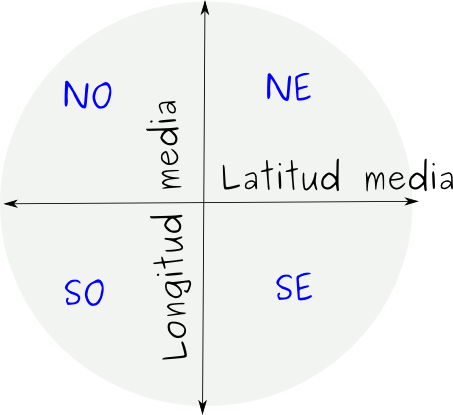
\includegraphics[width=1.66667in,height=1.66667in]{figuras/cuadrantes.png}
\caption{Cuadrantes definiddos por la posición media de longitud y latitud}
\end{figure}

Ayuda: se puede hacer un vector para las posiciones N -- S y otro para las posiciones E -- O. Luego mediante paste se pueden lograr todas las combinaciones posibles de cuadrantes

\begin{verbatim}
  Site lon lat  das alt  pen  deb  pH dur  pho  nit  amm  oxy dbo   sec
1    1  88   7  0.3 934 48.0 0.84 7.9  45 0.01 0.20 0.00 12.2 2.7 upper
2    2  94  14  2.2 932  3.0 1.00 8.0  40 0.02 0.20 0.10 10.3 1.9 upper
3    3 102  18 10.2 914  3.7 1.80 8.3  52 0.05 0.22 0.05 10.5 3.5 upper
4    4 100  28 18.5 854  3.2 2.53 8.0  72 0.10 0.21 0.00 11.0 1.3 upper
5    5 106  39 21.5 849  2.3 2.64 8.1  84 0.38 0.52 0.20  8.0 6.2 upper
6    6 112  51 32.4 846  3.2 2.86 7.9  60 0.20 0.15 0.00 10.2 5.3 upper
\end{verbatim}

\hypertarget{figura-cuadrantes-rrr}{%
\section{Figura cuadrantes (RRR)}\label{figura-cuadrantes-rrr}}

En base al resultado del punto anterior generar una figura como se muestra a continuación

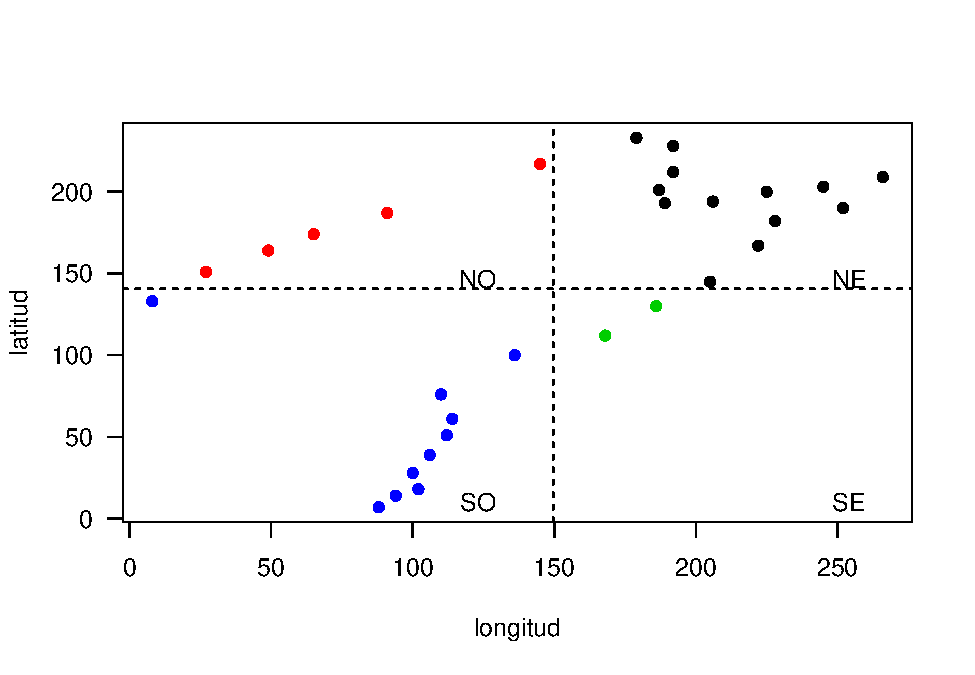
\includegraphics{R_ejercicios2021_files/figure-latex/unnamed-chunk-218-1.pdf}

Estructura

\begin{Shaded}
\begin{Highlighting}[]
\KeywordTok{plot}\NormalTok{(env}\OperatorTok{$}\NormalTok{lon, env}\OperatorTok{$}\NormalTok{lat, }\DataTypeTok{xlab=} \StringTok{"longitud"}\NormalTok{, }\DataTypeTok{ylab=} \StringTok{"latitud"}\NormalTok{, }\DataTypeTok{yaxt=}\StringTok{"n"}\NormalTok{, }\DataTypeTok{type=} \StringTok{"n"}\NormalTok{)}
  \KeywordTok{points}\NormalTok{(COMPLETAR, }\DataTypeTok{pch=} \DecValTok{16}\NormalTok{, }\DataTypeTok{col=} \StringTok{"red"}\NormalTok{)}
  \KeywordTok{points}\NormalTok{(COMPLETAR, }\DataTypeTok{pch=} \DecValTok{16}\NormalTok{, }\DataTypeTok{col=} \StringTok{"black"}\NormalTok{)}
  \KeywordTok{points}\NormalTok{(COMPLETAR, }\DataTypeTok{pch=} \DecValTok{16}\NormalTok{, }\DataTypeTok{col=} \StringTok{"green"}\NormalTok{)}
  \KeywordTok{points}\NormalTok{(COMPLETAR, }\DataTypeTok{pch=} \DecValTok{16}\NormalTok{, }\DataTypeTok{col=} \StringTok{"blue"}\NormalTok{)}
  \CommentTok{# eje x}
  \KeywordTok{axis}\NormalTok{(}\DataTypeTok{side=} \DecValTok{2}\NormalTok{, }\DataTypeTok{las=} \DecValTok{2}\NormalTok{)}
  \CommentTok{# líneas medias de lon y lat}
  \KeywordTok{abline}\NormalTok{(}\DataTypeTok{h=}\NormalTok{ COMPLETAR, }\DataTypeTok{lty=} \DecValTok{2}\NormalTok{)}
  \KeywordTok{abline}\NormalTok{(}\DataTypeTok{v=}\NormalTok{ COMPLETAR, }\DataTypeTok{lty=} \DecValTok{2}\NormalTok{)}
  \CommentTok{# leyendas de cuadrantes}
  \KeywordTok{par}\NormalTok{(}\DataTypeTok{usr=} \KeywordTok{c}\NormalTok{(}\DecValTok{0}\NormalTok{,}\DecValTok{10}\NormalTok{,}\DecValTok{0}\NormalTok{,}\DecValTok{10}\NormalTok{))}
  \KeywordTok{text}\NormalTok{(}\StringTok{"NE"}\NormalTok{, }\DataTypeTok{x=} \FloatTok{9.2}\NormalTok{, }\DataTypeTok{y=} \FloatTok{6.1}\NormalTok{)}
  \KeywordTok{text}\NormalTok{(}\StringTok{"NO"}\NormalTok{, }\DataTypeTok{x=} \FloatTok{4.5}\NormalTok{, }\DataTypeTok{y=} \FloatTok{6.1}\NormalTok{)}
  \KeywordTok{text}\NormalTok{(}\StringTok{"SE"}\NormalTok{, }\DataTypeTok{x=} \FloatTok{9.2}\NormalTok{, }\DataTypeTok{y=} \FloatTok{0.5}\NormalTok{)}
  \KeywordTok{text}\NormalTok{(}\StringTok{"SO"}\NormalTok{, }\DataTypeTok{x=} \FloatTok{4.5}\NormalTok{, }\DataTypeTok{y=} \FloatTok{0.5}\NormalTok{)}
\end{Highlighting}
\end{Shaded}

\hypertarget{if-rrr}{%
\section{if (RRR)}\label{if-rrr}}

Supongamos que queremos ejecutar la siguiente operación:

\begin{Shaded}
\begin{Highlighting}[]
\NormalTok{        x=}\StringTok{ }\DecValTok{1}\OperatorTok{:}\DecValTok{10}\NormalTok{  ; x}\OperatorTok{^}\DecValTok{2}  \CommentTok{# no hay ningún problema}
\end{Highlighting}
\end{Shaded}

\begin{verbatim}
##  [1]   1   4   9  16  25  36  49  64  81 100
\end{verbatim}

Pero si hacemos

\begin{Shaded}
\begin{Highlighting}[]
\NormalTok{      x=}\StringTok{ }\NormalTok{letters[}\DecValTok{1}\OperatorTok{:}\DecValTok{10}\NormalTok{]; x}\OperatorTok{^}\DecValTok{2} 
\end{Highlighting}
\end{Shaded}

Aparece un aviso de error \texttt{Error\ in\ x\^{}2\ :\ non-numeric\ argument\ to\ binary\ operator}

\begin{enumerate}
\def\labelenumi{\arabic{enumi}.}
\tightlist
\item
  Qué tal si armamos nuestro propio aviso de error?
\end{enumerate}

\begin{itemize}
\item
  Utilizar la función \emph{if()} para que aparezca un aviso de error cuando la variable no sea numérica. Por ejemplo que diga ``ESTA OPERACIÓN NO FUNCIONA PARA VARIABLES NO NUMÉRICAS''
\item
  Un paso un poco más ambicioso es que además nos aparezca en consola un mensaje que nos indique de que clase es el objeto al que erroneamente intentamos aplicar la operación. \textbf{Ayuda}: combinar \textbf{paste()} y \textbf{class()}
\end{itemize}

\hypertarget{if-plot-rrr}{%
\section{if + plot (RRR)}\label{if-plot-rrr}}

Utilizar la función \emph{if()} para generar una figura a partir de los valores de un único vector. Si el vector es de clase \emph{integer} (números enteros) la figura será un histograma, mientras que si el vector es de clase \emph{numeric} (números reales) se graficará un boxplot con los valores del vector. Generar los comandos y ponerlos a prueba con los vectores que se dan a continuación

\begin{Shaded}
\begin{Highlighting}[]
\NormalTok{x <-}\StringTok{ }\KeywordTok{as.integer}\NormalTok{( }\KeywordTok{sample}\NormalTok{(}\DecValTok{1}\OperatorTok{:}\DecValTok{100}\NormalTok{, }\DecValTok{100}\NormalTok{, }\DataTypeTok{replace=}\NormalTok{T) )}
\KeywordTok{class}\NormalTok{ (x)}
\end{Highlighting}
\end{Shaded}

\begin{verbatim}
## [1] "integer"
\end{verbatim}

\begin{Shaded}
\begin{Highlighting}[]
\NormalTok{x <-}\StringTok{ }\KeywordTok{seq}\NormalTok{(}\DecValTok{1}\NormalTok{, }\DecValTok{10}\NormalTok{, }\FloatTok{0.5}\NormalTok{)}
\KeywordTok{class}\NormalTok{(x)}
\end{Highlighting}
\end{Shaded}

\begin{verbatim}
## [1] "numeric"
\end{verbatim}

\hypertarget{r14-funciones}{%
\chapter*{R14 Funciones}\label{r14-funciones}}
\addcontentsline{toc}{chapter}{R14 Funciones}

\hypertarget{funciones-elevar-al-cuadrado-r}{%
\section{Funciones: elevar al cuadrado (R)}\label{funciones-elevar-al-cuadrado-r}}

\begin{itemize}
\tightlist
\item
  Escribir una función que llamaremos \textbf{elev2} que calcule el cuadrado de una serie de números
\item
  La función debe devolver en un data.frame con los números de ingreso y sus correspondientes valores al cuadrados
\end{itemize}

\begin{Shaded}
\begin{Highlighting}[]
\NormalTok{  x <-}\DecValTok{1}\OperatorTok{:}\DecValTok{10}
  \KeywordTok{elev2}\NormalTok{(x) }
\end{Highlighting}
\end{Shaded}

\begin{verbatim}
    x  x2
1   1   1
2   2   4
3   3   9
4   4  16
5   5  25
6   6  36
7   7  49
8   8  64
9   9  81
10 10 100
\end{verbatim}

Estructura

\begin{Shaded}
\begin{Highlighting}[]
\NormalTok{elev2 <-}\StringTok{ }\ControlFlowTok{function}\NormalTok{(completar) \{}
\NormalTok{  y <-}\StringTok{ }\NormalTok{COMPLETAR }\OperatorTok{^}\DecValTok{2}
  \KeywordTok{data.frame}\NormalTok{(}\DataTypeTok{x=}\NormalTok{ x, }\DataTypeTok{x2 =}\NormalTok{ y)}
\NormalTok{  \}}
\end{Highlighting}
\end{Shaded}

\hypertarget{funciones-elevar-al-cuadrado-2-rrr}{%
\section{Funciones: elevar al cuadrado 2 (RRR)}\label{funciones-elevar-al-cuadrado-2-rrr}}

\begin{itemize}
\tightlist
\item
  Agregar a la estructura de la función anterior un ``control'', para que en los casos en que el vector de ingreso no sea numérico aparezca un cartel que diga ``ERROR: Los datos de ingreso no son numéricos''
\end{itemize}

\begin{Shaded}
\begin{Highlighting}[]
\NormalTok{  x <-}\KeywordTok{c}\NormalTok{(}\DecValTok{1}\OperatorTok{:}\DecValTok{10}\NormalTok{, }\OtherTok{NA}\NormalTok{, }\OtherTok{NA}\NormalTok{, }\OtherTok{NA}\NormalTok{)}
  \KeywordTok{elev2}\NormalTok{(x) }
\end{Highlighting}
\end{Shaded}

\begin{verbatim}
    x  x2
1   1   1
2   2   4
3   3   9
4   4  16
5   5  25
6   6  36
7   7  49
8   8  64
9   9  81
10 10 100
11 NA  NA
12 NA  NA
13 NA  NA
\end{verbatim}

\begin{Shaded}
\begin{Highlighting}[]
\NormalTok{  y <-}\StringTok{ }\NormalTok{letters}
  \KeywordTok{elev2}\NormalTok{(y)}
\end{Highlighting}
\end{Shaded}

\begin{verbatim}
[1] "ERROR: Los datos de ingreso no son numéricos"
\end{verbatim}

Estructura

\begin{Shaded}
\begin{Highlighting}[]
\NormalTok{elev2 <-}\StringTok{ }\ControlFlowTok{function}\NormalTok{(COMPLETAR) \{}
      \ControlFlowTok{if}\NormalTok{(COMPLETAR) \{}
\NormalTok{        COMPLETAR CON COMANDOS SI T}
\NormalTok{        \} }\ControlFlowTok{else}\NormalTok{ \{}
\NormalTok{        COMPLETAR CON COMANDOS SI F}
\NormalTok{       \}}
\NormalTok{    \}}
\end{Highlighting}
\end{Shaded}

\hypertarget{funciones-promedio-rr}{%
\section{Funciones: Promedio (RR)}\label{funciones-promedio-rr}}

Generar una función a la que llamaremos ``promedio'', que calculará el valor promedio de un vector numérico como:\\
\[promedio = \frac{\sum x_{i}}{N}\]

Donde N es número de elementos del vector x (length(x))
Por el momento la función tendrá un único argumento \emph{x} y no estará definida para vectores con NA's

Por ejemplo:

\begin{Shaded}
\begin{Highlighting}[]
\NormalTok{y <-}\StringTok{ }\KeywordTok{c}\NormalTok{(}\DecValTok{3}\NormalTok{, }\DecValTok{5}\NormalTok{, }\DecValTok{4}\NormalTok{, }\OtherTok{NA}\NormalTok{, }\OtherTok{NA}\NormalTok{, }\DecValTok{8}\NormalTok{)}
\KeywordTok{promedio}\NormalTok{(y)}
\end{Highlighting}
\end{Shaded}

\begin{verbatim}
## [1] NA
\end{verbatim}

\begin{Shaded}
\begin{Highlighting}[]
\CommentTok{# En este caso el resultado es NA porque sum(x) = NA}

\NormalTok{z <-}\StringTok{ }\KeywordTok{c}\NormalTok{(}\DecValTok{3}\NormalTok{, }\DecValTok{5}\NormalTok{, }\DecValTok{4}\NormalTok{, }\DecValTok{4}\NormalTok{, }\DecValTok{5}\NormalTok{, }\DecValTok{8}\NormalTok{)}
\KeywordTok{promedio}\NormalTok{(z)}
\end{Highlighting}
\end{Shaded}

\begin{verbatim}
## [1] 4.833333
\end{verbatim}

\hypertarget{funciones-promedio-2-rrr}{%
\section{Funciones: Promedio 2 (RRR)}\label{funciones-promedio-2-rrr}}

Generar la misma función que en el punto anterior pero con un argumento extra que permita eliminar los valores NA para el cálculo del promedio

\begin{Shaded}
\begin{Highlighting}[]
\NormalTok{y <-}\StringTok{ }\KeywordTok{c}\NormalTok{(}\DecValTok{3}\NormalTok{, }\DecValTok{5}\NormalTok{, }\DecValTok{4}\NormalTok{, }\OtherTok{NA}\NormalTok{, }\OtherTok{NA}\NormalTok{, }\DecValTok{8}\NormalTok{)}
\KeywordTok{promedio}\NormalTok{(y)}
\end{Highlighting}
\end{Shaded}

\begin{verbatim}
## [1] 5
\end{verbatim}

\hypertarget{funciuxf3n-obtener-nuxfameros-pares-o-impares}{%
\section{Función obtener números pares o impares}\label{funciuxf3n-obtener-nuxfameros-pares-o-impares}}

Dado un vector numérico cualquiera, como el que se muestra a continuación:

\begin{Shaded}
\begin{Highlighting}[]
\NormalTok{x <-}\StringTok{ }\KeywordTok{c}\NormalTok{(}\DecValTok{1}\NormalTok{,}\DecValTok{2}\NormalTok{,}\DecValTok{5}\NormalTok{,}\DecValTok{7}\NormalTok{,}\DecValTok{9}\NormalTok{,}\DecValTok{8}\NormalTok{,}\DecValTok{2}\NormalTok{,}\DecValTok{51}\NormalTok{)}
\end{Highlighting}
\end{Shaded}

Mediante el siguiente comando se puede obtener un vector de 1's y 0's para aquellos valores impares y pares del vector

\begin{Shaded}
\begin{Highlighting}[]
\NormalTok{x }\OperatorTok\StringTok{ }\DecValTok{2}
\end{Highlighting}
\end{Shaded}

\begin{verbatim}
## [1] 1 0 1 1 1 0 0 1
\end{verbatim}

Generar una función, que llamaremos \textbf{\textbf{parimpar}} que permita obtener los valores pares o impares de un vector numérico. La función deberá tener dos argumentos, el primero, al que llamaremos \textbf{\textbf{vec}}, corresponderá al vector de entrada y el segundo al que llamaremos impar tomará valor por defecto TRUE y seleccionará a los valores impares, mientras que seleccionará a los pares en caso de ser FALSE

Pasos sugeridos
* generar un vector lógico (idx1) con la condición vec \%\% 2 == 1 (impares)
* generar un vector lógico (idx2) con la condición vec \%\% 2 == 0 (pares)
* incluir un condicional que indexe por idx1 en caso de que el parámetro impar sea T y que indexe por idx2 en caso contrario

Probando la función

\begin{Shaded}
\begin{Highlighting}[]
\NormalTok{x <-}\StringTok{ }\KeywordTok{c}\NormalTok{(}\DecValTok{1}\NormalTok{,}\DecValTok{2}\NormalTok{,}\DecValTok{5}\NormalTok{,}\DecValTok{7}\NormalTok{,}\DecValTok{9}\NormalTok{,}\DecValTok{8}\NormalTok{,}\DecValTok{2}\NormalTok{,}\DecValTok{51}\NormalTok{)}

\KeywordTok{parimpar}\NormalTok{(x)}
\end{Highlighting}
\end{Shaded}

\begin{verbatim}
## [1]  1  2  9  2 NA 51  2 NA
\end{verbatim}

\begin{Shaded}
\begin{Highlighting}[]
\KeywordTok{parimpar}\NormalTok{(x, F)}
\end{Highlighting}
\end{Shaded}

\begin{verbatim}
## [1] 2 8 2
\end{verbatim}

\hypertarget{funciones-no-contar-los-nas-rrr}{%
\section{Funciones: No contar los NAs (RRR)}\label{funciones-no-contar-los-nas-rrr}}

Las funciones de la familia \textbf{\emph{apply}} no tienen argumentos para eliminar los NA's de los resultados cuando se usa \textbf{\emph{length()}}
Ejemplo

\begin{Shaded}
\begin{Highlighting}[]
\NormalTok{    x <-}\StringTok{ }\KeywordTok{c}\NormalTok{( }\DecValTok{1}\OperatorTok{:}\DecValTok{20}\NormalTok{, }\KeywordTok{rep}\NormalTok{(}\OtherTok{NA}\NormalTok{, }\DecValTok{4}\NormalTok{) )}
\NormalTok{    x}
\end{Highlighting}
\end{Shaded}

\begin{verbatim}
 [1]  1  2  3  4  5  6  7  8  9 10 11 12 13 14 15 16 17 18 19 20 NA NA NA NA
\end{verbatim}

\begin{Shaded}
\begin{Highlighting}[]
\NormalTok{        y <-}\StringTok{ }\KeywordTok{rep}\NormalTok{( }\KeywordTok{c}\NormalTok{(}\StringTok{"A"}\NormalTok{, }\StringTok{"B"}\NormalTok{), }\DataTypeTok{each=}\DecValTok{12}\NormalTok{) }
\NormalTok{    y}
\end{Highlighting}
\end{Shaded}

\begin{verbatim}
 [1] "A" "A" "A" "A" "A" "A" "A" "A" "A" "A" "A" "A" "B" "B" "B" "B" "B" "B" "B"
[20] "B" "B" "B" "B" "B"
\end{verbatim}

\begin{Shaded}
\begin{Highlighting}[]
\NormalTok{        z <-}\StringTok{ }\KeywordTok{data.frame}\NormalTok{(}\DataTypeTok{pob=}\NormalTok{y,}\DataTypeTok{x=}\NormalTok{x)}
\NormalTok{    z}
\end{Highlighting}
\end{Shaded}

\begin{verbatim}
   pob  x
1    A  1
2    A  2
3    A  3
4    A  4
5    A  5
6    A  6
7    A  7
8    A  8
9    A  9
10   A 10
11   A 11
12   A 12
13   B 13
14   B 14
15   B 15
16   B 16
17   B 17
18   B 18
19   B 19
20   B 20
21   B NA
22   B NA
23   B NA
24   B NA
\end{verbatim}

\begin{Shaded}
\begin{Highlighting}[]
        \KeywordTok{tapply}\NormalTok{(z}\OperatorTok{$}\NormalTok{x, z}\OperatorTok{$}\NormalTok{pob, mean, }\DataTypeTok{na.rm=}\NormalTok{T) }\CommentTok{#esto funciona}
\end{Highlighting}
\end{Shaded}

\begin{verbatim}
   A    B 
 6.5 16.5 
\end{verbatim}

\begin{Shaded}
\begin{Highlighting}[]
    \KeywordTok{tapply}\NormalTok{(z}\OperatorTok{$}\NormalTok{x, z}\OperatorTok{$}\NormalTok{pob, length) }\CommentTok{#esto funciona pero cuenta los NA's}
\end{Highlighting}
\end{Shaded}

\begin{verbatim}
 A  B 
12 12 
\end{verbatim}

\begin{enumerate}
\def\labelenumi{\arabic{enumi}.}
\tightlist
\item
  Generemos entonces una función que llamaremos \textbf{\emph{sinNA}} para usar funciones de la familia \textbf{\emph{apply}} y que no cuente los NA's
\end{enumerate}

La salida de tapply() usando la función debería dar:

\begin{Shaded}
\begin{Highlighting}[]
    \KeywordTok{tapply}\NormalTok{(z}\OperatorTok{$}\NormalTok{x, z}\OperatorTok{$}\NormalTok{pob, sinNA)}
\end{Highlighting}
\end{Shaded}

\begin{verbatim}
##  A  B 
## 12  8
\end{verbatim}

\hypertarget{funciuxf3n-frecuencia-relativa-rrr}{%
\section{Función frecuencia relativa (RRR)}\label{funciuxf3n-frecuencia-relativa-rrr}}

Muchas veces es necesario expresar valores de tablas en forma de frecuencia relativa. Es decir, pasar valores absolutos de observaciones a formato de frecuencia

\begin{quote}
FR = \(\frac{Ni}{N}*100\)
\end{quote}

Donde Ni es el valor de la celda i y N es la suma de todos los valores del vector

Los siguientes comandos generan datos simulados de 5 poblaciones de una especie hipotética de depredador que consume 5 tipos de presa.

\begin{Shaded}
\begin{Highlighting}[]
\NormalTok{  presas <-}\StringTok{ }\KeywordTok{paste}\NormalTok{(}\StringTok{"presa"}\NormalTok{, }\DecValTok{1}\OperatorTok{:}\DecValTok{5}\NormalTok{)}
\NormalTok{  pobl <-}\StringTok{ }\KeywordTok{paste}\NormalTok{(}\StringTok{"pob"}\NormalTok{, }\DecValTok{1}\OperatorTok{:}\DecValTok{5}\NormalTok{)}
  \KeywordTok{set.seed}\NormalTok{(}\DecValTok{300}\NormalTok{)}
\NormalTok{  datos <-}\StringTok{ }\KeywordTok{round}\NormalTok{( }\KeywordTok{runif}\NormalTok{(}\DecValTok{25}\NormalTok{, }\DecValTok{1}\NormalTok{, }\DecValTok{100}\NormalTok{), }\DecValTok{0}\NormalTok{)}
\NormalTok{  tabla <-}\StringTok{ }\KeywordTok{matrix}\NormalTok{(datos, }\DataTypeTok{ncol=}\DecValTok{5}\NormalTok{, }\DataTypeTok{dimnames=}\KeywordTok{list}\NormalTok{(presas, pobl))}
\NormalTok{  tabla}
\end{Highlighting}
\end{Shaded}

\begin{verbatim}
##         pob 1 pob 2 pob 3 pob 4 pob 5
## presa 1    92     2    94    99    99
## presa 2    77    76    33    89    50
## presa 3    81    50    80    67    47
## presa 4    74    47    59    64     7
## presa 5    69    90    66    51    10
\end{verbatim}

\begin{enumerate}
\def\labelenumi{\arabic{enumi}.}
\tightlist
\item
  El ejercicio consiste en estimar el índice de frecuencia relativa de las presas para cada ejemplar. Para ello, generaremos una función (\textbf{FR}) que calcule la frecuencia de ocurrencia en base a un vector de observaciones. Finalmente, la función será utilizada como argumento de la función de resumen en el ejercicio que sigue.
\end{enumerate}

Aplicando la función recién creada a la primera fila de la tabla debería dar el siguiente resultado

\begin{Shaded}
\begin{Highlighting}[]
\NormalTok{prueba <-}\StringTok{ }\KeywordTok{FR}\NormalTok{(tabla[}\DecValTok{1}\NormalTok{, ])}
\NormalTok{prueba}
\end{Highlighting}
\end{Shaded}

\begin{verbatim}
##      pob 1      pob 2      pob 3      pob 4      pob 5 
## 23.8341969  0.5181347 24.3523316 25.6476684 25.6476684
\end{verbatim}

\begin{Shaded}
\begin{Highlighting}[]
\KeywordTok{sum}\NormalTok{(prueba)}
\end{Highlighting}
\end{Shaded}

\begin{verbatim}
## [1] 100
\end{verbatim}

La tabla de salida debería verse como la siguiente (los valores obtenidos fueron redondeados ( \textbf{\emph{round()}} ) a dos decimales)

\begin{Shaded}
\begin{Highlighting}[]
\NormalTok{salida <-}\StringTok{ }\KeywordTok{round}\NormalTok{ (}\KeywordTok{apply}\NormalTok{(tabla, }\DecValTok{1}\NormalTok{, FR), }\DecValTok{2}\NormalTok{)}
\NormalTok{salida}
\end{Highlighting}
\end{Shaded}

\begin{verbatim}
##       presa 1 presa 2 presa 3 presa 4 presa 5
## pob 1   23.83   23.69   24.92   29.48   24.13
## pob 2    0.52   23.38   15.38   18.73   31.47
## pob 3   24.35   10.15   24.62   23.51   23.08
## pob 4   25.65   27.38   20.62   25.50   17.83
## pob 5   25.65   15.38   14.46    2.79    3.50
\end{verbatim}

\begin{Shaded}
\begin{Highlighting}[]
\KeywordTok{colSums}\NormalTok{(salida) }\CommentTok{## la suma de las frecuencias realtivas por columna debe dar 1}
\end{Highlighting}
\end{Shaded}

\begin{verbatim}
## presa 1 presa 2 presa 3 presa 4 presa 5 
##  100.00   99.98  100.00  100.01  100.01
\end{verbatim}

--\textgreater{}

\hypertarget{debugging-detectando-errores-7}{%
\section{Debugging, detectando errores}\label{debugging-detectando-errores-7}}

Correr las siguientes líneas de comando para generar datos de prueba. Examinar cada uno de los objetos

\begin{Shaded}
\begin{Highlighting}[]
\KeywordTok{rm}\NormalTok{( }\DataTypeTok{list =} \KeywordTok{ls}\NormalTok{() ) }\CommentTok{#eliminemos primero todos los objetos}
\end{Highlighting}
\end{Shaded}

\begin{Shaded}
\begin{Highlighting}[]
\NormalTok{  x <-}\StringTok{ }\KeywordTok{runif}\NormalTok{(}\DecValTok{100}\NormalTok{,}\DecValTok{10}\NormalTok{, }\DecValTok{100}\NormalTok{)}
\NormalTok{    y <-}\StringTok{ }\KeywordTok{rnorm}\NormalTok{(}\DecValTok{100}\NormalTok{, }\DecValTok{10}\NormalTok{ ,}\DecValTok{100}\NormalTok{)}
\NormalTok{        z <-}\StringTok{ }\KeywordTok{seq}\NormalTok{(}\DecValTok{0}\NormalTok{,}\DecValTok{200}\NormalTok{, }\DecValTok{2}\NormalTok{)}
\NormalTok{        g  <-}\StringTok{ }\KeywordTok{sample}\NormalTok{(letters,}\DecValTok{100}\NormalTok{,T)}

\NormalTok{        tabla <-}\StringTok{ }\KeywordTok{data.frame}\NormalTok{(x,y,g)}
\NormalTok{        matriz <-}\StringTok{ }\KeywordTok{matrix}\NormalTok{(}\KeywordTok{c}\NormalTok{(x,y,g), }\DataTypeTok{ncol=}\DecValTok{3}\NormalTok{)}
\NormalTok{        lista <-}\StringTok{ }\KeywordTok{list}\NormalTok{(tabla, matriz)}
\end{Highlighting}
\end{Shaded}

Para cada una de las siguientes líneas de código explicar por que se obtiene un mensaje de error, warnning, o un resultado no esperado

\begin{enumerate}
\def\labelenumi{\arabic{enumi}.}
\item
\end{enumerate}

\begin{Shaded}
\begin{Highlighting}[]
\NormalTok{mm <-}\StringTok{ }\KeywordTok{ifelse}\NormalTok{(x }\OperatorTok{>=}\StringTok{ }\DecValTok{23} \OperatorTok{&}\StringTok{ }\DataTypeTok{y =}\OperatorTok{<}\StringTok{ }\DecValTok{5}\NormalTok{, }\StringTok{"target"}\NormalTok{, }\OtherTok{NA}\NormalTok{)}
\end{Highlighting}
\end{Shaded}

\begin{enumerate}
\def\labelenumi{\arabic{enumi}.}
\setcounter{enumi}{1}
\item
\end{enumerate}

\begin{Shaded}
\begin{Highlighting}[]
\KeywordTok{log}\NormalTok{(y)}
\end{Highlighting}
\end{Shaded}

\begin{enumerate}
\def\labelenumi{\arabic{enumi}.}
\setcounter{enumi}{2}
\item
\end{enumerate}

\begin{Shaded}
\begin{Highlighting}[]
\KeywordTok{dim.names}\NormalTok{(tabla)}
\end{Highlighting}
\end{Shaded}

\begin{enumerate}
\def\labelenumi{\arabic{enumi}.}
\setcounter{enumi}{3}
\item
\end{enumerate}

\begin{Shaded}
\begin{Highlighting}[]
\ControlFlowTok{if}\NormalTok{(}\KeywordTok{is.numeric}\NormalTok{(x)) }\KeywordTok{hist}\NormalTok{(x) }\KeywordTok{print}\NormalTok{(}\StringTok{"la variable no es numerica"}\NormalTok{)}
\end{Highlighting}
\end{Shaded}

\begin{enumerate}
\def\labelenumi{\arabic{enumi}.}
\setcounter{enumi}{3}
\item
\end{enumerate}

\begin{Shaded}
\begin{Highlighting}[]
\ControlFlowTok{if}\NormalTok{(}\KeywordTok{is.numeric}\NormalTok{(g))\{}
    \KeywordTok{hist}\NormalTok{(g) }
\NormalTok{        \} }\ControlFlowTok{else} 
        \KeywordTok{print}\NormalTok{(}\StringTok{"la variable no es numerica"}\NormalTok{)}
  \ErrorTok{\}}
\end{Highlighting}
\end{Shaded}

\begin{enumerate}
\def\labelenumi{\arabic{enumi}.}
\setcounter{enumi}{4}
\item
\end{enumerate}

\begin{Shaded}
\begin{Highlighting}[]
\ControlFlowTok{if}\NormalTok{(x}\OperatorTok{>}\DecValTok{5}\NormalTok{) }\StringTok{"grande"} \ControlFlowTok{else} \StringTok{"chico"}
\end{Highlighting}
\end{Shaded}

\hypertarget{r15-loops}{%
\chapter*{R15 Loops}\label{r15-loops}}
\addcontentsline{toc}{chapter}{R15 Loops}

\hypertarget{loops-paso-a-paso}{%
\section{Loops: paso a paso}\label{loops-paso-a-paso}}

En este ejemplo vamos a analizar la conveniencia de utilizar loops cuando realizamos tareas repetida.

Supongamos que tenemos los siguientes datos

\begin{Shaded}
\begin{Highlighting}[]
\NormalTok{x <-}\StringTok{ }\KeywordTok{matrix}\NormalTok{(}\KeywordTok{rnorm}\NormalTok{(}\DecValTok{1000}\NormalTok{, }\DecValTok{10}\NormalTok{, }\DecValTok{1}\NormalTok{), }\DataTypeTok{ncol=} \DecValTok{10}\NormalTok{) }\CommentTok{# una matríz de diez columnas, con números aleatorios con distribución de error normal con media 10 y varianza 1}
\end{Highlighting}
\end{Shaded}

Ahora queremos generar una figura compuesta con histogramas de los valores de cada una de las columnas de x, indicando en cada figura cuál es la columna que se está graficando. Para lo cual generamos una ventana grafica y damos los comandos de diez histogramas, como se muestra a continuación.

\begin{Shaded}
\begin{Highlighting}[]
\NormalTok{nombres <-}\StringTok{ }\KeywordTok{paste}\NormalTok{(}\StringTok{"columna"}\NormalTok{, }\DecValTok{1}\OperatorTok{:}\DecValTok{10}\NormalTok{) }\CommentTok{# rótulo para indicar cuál es la columna que se está graficando}
\end{Highlighting}
\end{Shaded}

\begin{Shaded}
\begin{Highlighting}[]
\ControlFlowTok{if}\NormalTok{ (}\KeywordTok{Sys.info}\NormalTok{()[}\StringTok{'sysname'}\NormalTok{] }\OperatorTok{==}\StringTok{ "Windows"}\NormalTok{) }\KeywordTok{windows}\NormalTok{() }\ControlFlowTok{else} \KeywordTok{x11}\NormalTok{() }\CommentTok{## abre una ventana gráfica usando la función windows() si tu sistema operativo es windows() o x11() si tu sistema operativo es linux}

\KeywordTok{par}\NormalTok{(}\DataTypeTok{mfrow =} \KeywordTok{c}\NormalTok{(}\DecValTok{5}\NormalTok{,}\DecValTok{2}\NormalTok{), }\DataTypeTok{mar=} \KeywordTok{c}\NormalTok{(}\DecValTok{3}\NormalTok{, }\DecValTok{3}\NormalTok{, }\DecValTok{1}\NormalTok{, }\DecValTok{1}\NormalTok{))}
\CommentTok{#figura 1}
\KeywordTok{hist}\NormalTok{(x[ ,}\DecValTok{1}\NormalTok{], }\DataTypeTok{main=} \StringTok{""}\NormalTok{)}
\KeywordTok{par}\NormalTok{(}\DataTypeTok{usr=} \KeywordTok{c}\NormalTok{(}\DecValTok{0}\NormalTok{,}\DecValTok{10}\NormalTok{,}\DecValTok{0}\NormalTok{,}\DecValTok{10}\NormalTok{)) }\CommentTok{#redefinimos los ejes para poner el rótulo en la misma posición en todas las figuras.}
\KeywordTok{text}\NormalTok{(}\DataTypeTok{x=} \DecValTok{2}\NormalTok{, }\DataTypeTok{y=} \DecValTok{8}\NormalTok{, nombres[}\DecValTok{1}\NormalTok{]) }\CommentTok{#rótulo indicando la columna que se está graficando}

\CommentTok{#figura 2}
\KeywordTok{hist}\NormalTok{(x[ ,}\DecValTok{2}\NormalTok{], }\DataTypeTok{main=} \StringTok{""}\NormalTok{)}
\KeywordTok{par}\NormalTok{(}\DataTypeTok{usr=} \KeywordTok{c}\NormalTok{(}\DecValTok{0}\NormalTok{,}\DecValTok{10}\NormalTok{,}\DecValTok{0}\NormalTok{,}\DecValTok{10}\NormalTok{))}
\KeywordTok{text}\NormalTok{(}\DataTypeTok{x=} \DecValTok{2}\NormalTok{, }\DataTypeTok{y=} \DecValTok{8}\NormalTok{, nombres[}\DecValTok{2}\NormalTok{])}

\CommentTok{#figura 3}
\KeywordTok{hist}\NormalTok{(x[ ,}\DecValTok{3}\NormalTok{], }\DataTypeTok{main=} \StringTok{""}\NormalTok{)}
\KeywordTok{par}\NormalTok{(}\DataTypeTok{usr=} \KeywordTok{c}\NormalTok{(}\DecValTok{0}\NormalTok{,}\DecValTok{10}\NormalTok{,}\DecValTok{0}\NormalTok{,}\DecValTok{10}\NormalTok{))}
\KeywordTok{text}\NormalTok{(}\DataTypeTok{x=} \DecValTok{2}\NormalTok{, }\DataTypeTok{y=} \DecValTok{8}\NormalTok{, nombres[}\DecValTok{3}\NormalTok{])}

\CommentTok{#figura 4}
\KeywordTok{hist}\NormalTok{(x[ ,}\DecValTok{4}\NormalTok{], }\DataTypeTok{main=} \StringTok{""}\NormalTok{)}
\KeywordTok{par}\NormalTok{(}\DataTypeTok{usr=} \KeywordTok{c}\NormalTok{(}\DecValTok{0}\NormalTok{,}\DecValTok{10}\NormalTok{,}\DecValTok{0}\NormalTok{,}\DecValTok{10}\NormalTok{))}
\KeywordTok{text}\NormalTok{(}\DataTypeTok{x=} \DecValTok{2}\NormalTok{, }\DataTypeTok{y=} \DecValTok{8}\NormalTok{, nombres[}\DecValTok{4}\NormalTok{])}

\CommentTok{#figura 5}
\KeywordTok{hist}\NormalTok{(x[ ,}\DecValTok{5}\NormalTok{], }\DataTypeTok{main=} \StringTok{""}\NormalTok{)}
\KeywordTok{par}\NormalTok{(}\DataTypeTok{usr=} \KeywordTok{c}\NormalTok{(}\DecValTok{0}\NormalTok{,}\DecValTok{10}\NormalTok{,}\DecValTok{0}\NormalTok{,}\DecValTok{10}\NormalTok{))}
\KeywordTok{text}\NormalTok{(}\DataTypeTok{x=} \DecValTok{2}\NormalTok{, }\DataTypeTok{y=} \DecValTok{8}\NormalTok{, nombres[}\DecValTok{5}\NormalTok{])}

\CommentTok{#figura 6}
\KeywordTok{hist}\NormalTok{(x[ ,}\DecValTok{6}\NormalTok{], }\DataTypeTok{main=} \StringTok{""}\NormalTok{)}
\KeywordTok{par}\NormalTok{(}\DataTypeTok{usr=} \KeywordTok{c}\NormalTok{(}\DecValTok{0}\NormalTok{,}\DecValTok{10}\NormalTok{,}\DecValTok{0}\NormalTok{,}\DecValTok{10}\NormalTok{))}
\KeywordTok{text}\NormalTok{(}\DataTypeTok{x=} \DecValTok{2}\NormalTok{, }\DataTypeTok{y=} \DecValTok{8}\NormalTok{, nombres[}\DecValTok{6}\NormalTok{])}

\CommentTok{#figura 7}
\KeywordTok{hist}\NormalTok{(x[ ,}\DecValTok{7}\NormalTok{], }\DataTypeTok{main=} \StringTok{""}\NormalTok{)}
\KeywordTok{par}\NormalTok{(}\DataTypeTok{usr=} \KeywordTok{c}\NormalTok{(}\DecValTok{0}\NormalTok{,}\DecValTok{10}\NormalTok{,}\DecValTok{0}\NormalTok{,}\DecValTok{10}\NormalTok{))}
\KeywordTok{text}\NormalTok{(}\DataTypeTok{x=} \DecValTok{2}\NormalTok{, }\DataTypeTok{y=} \DecValTok{8}\NormalTok{, nombres[}\DecValTok{7}\NormalTok{])}

\CommentTok{#figura 8}
\KeywordTok{hist}\NormalTok{(x[ ,}\DecValTok{8}\NormalTok{], }\DataTypeTok{main=} \StringTok{""}\NormalTok{)}
\KeywordTok{par}\NormalTok{(}\DataTypeTok{usr=} \KeywordTok{c}\NormalTok{(}\DecValTok{0}\NormalTok{,}\DecValTok{10}\NormalTok{,}\DecValTok{0}\NormalTok{,}\DecValTok{10}\NormalTok{))}
\KeywordTok{text}\NormalTok{(}\DataTypeTok{x=} \DecValTok{2}\NormalTok{, }\DataTypeTok{y=} \DecValTok{8}\NormalTok{, nombres[}\DecValTok{8}\NormalTok{])}

\CommentTok{#figura 9}
\KeywordTok{hist}\NormalTok{(x[ ,}\DecValTok{9}\NormalTok{], }\DataTypeTok{main=} \StringTok{""}\NormalTok{)}
\KeywordTok{par}\NormalTok{(}\DataTypeTok{usr=} \KeywordTok{c}\NormalTok{(}\DecValTok{0}\NormalTok{,}\DecValTok{10}\NormalTok{,}\DecValTok{0}\NormalTok{,}\DecValTok{10}\NormalTok{))}
\KeywordTok{text}\NormalTok{(}\DataTypeTok{x=} \DecValTok{2}\NormalTok{, }\DataTypeTok{y=} \DecValTok{8}\NormalTok{, nombres[}\DecValTok{9}\NormalTok{])}

\CommentTok{#figura 10}
\KeywordTok{hist}\NormalTok{(x[ ,}\DecValTok{10}\NormalTok{], }\DataTypeTok{main=} \StringTok{""}\NormalTok{)}
\KeywordTok{par}\NormalTok{(}\DataTypeTok{usr=} \KeywordTok{c}\NormalTok{(}\DecValTok{0}\NormalTok{,}\DecValTok{10}\NormalTok{,}\DecValTok{0}\NormalTok{,}\DecValTok{10}\NormalTok{))}
\KeywordTok{text}\NormalTok{(}\DataTypeTok{x=} \DecValTok{2}\NormalTok{, }\DataTypeTok{y=} \DecValTok{8}\NormalTok{, nombres[}\DecValTok{10}\NormalTok{])}
\end{Highlighting}
\end{Shaded}

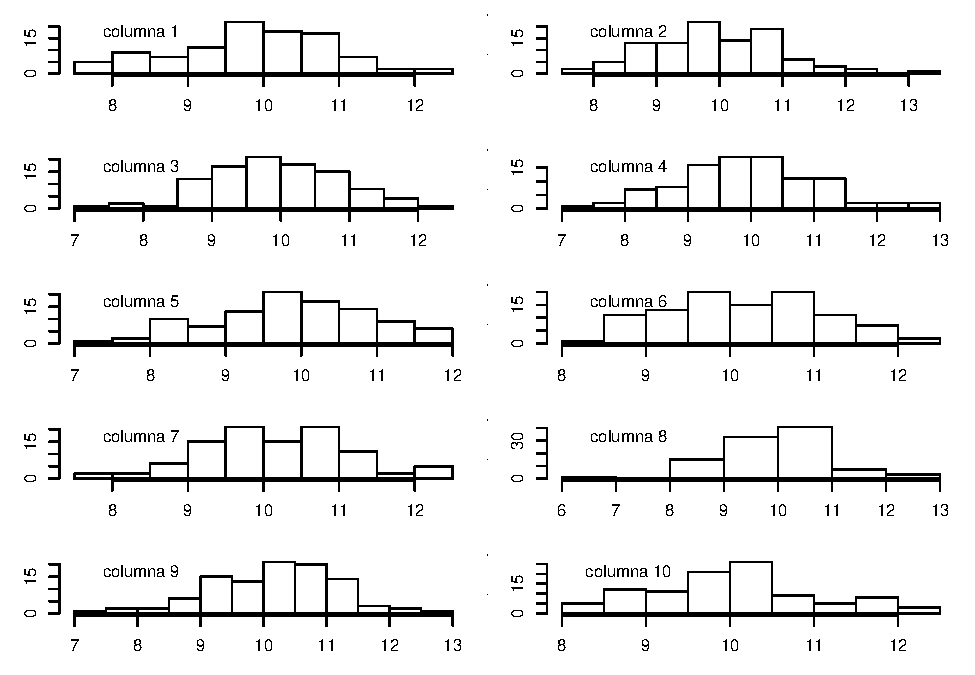
\includegraphics{R_ejercicios2021_files/figure-latex/unnamed-chunk-259-1.pdf}

Muy bien, para hacerlo escribimos los comandos para hacer un histograma, luego lo copiamos 9 veces y reemplazamos en la indexación de cada caso por la columna y el nombre de la columna correspondiente. NO es tanto trabajo después de todo. Sin embargo, ahora vemos que la leyendas de los ejes no son las que nos gustaría tener, y el color no nos convence. Tendríamos entonces que editar uno por uno los comandos para modificar cada histograma. Esto además de ser tedioso aumenta las chances de que cometamos errores.

Una opción un poco más saludable es generar una sola vez los comandos e ir cambiando los valores de indexación (donde dice REEMPLAZAR en el código que sigue). Cada vez que lo corramos se irán completando los paneles de nuestra figura múltiple hasta que completemos los 10 histogramas

\begin{Shaded}
\begin{Highlighting}[]
\ControlFlowTok{if}\NormalTok{ (}\KeywordTok{Sys.info}\NormalTok{()[}\StringTok{'sysname'}\NormalTok{] }\OperatorTok{==}\StringTok{ "Windows"}\NormalTok{) }\KeywordTok{windows}\NormalTok{() }\ControlFlowTok{else} \KeywordTok{x11}\NormalTok{() }

\KeywordTok{par}\NormalTok{(}\DataTypeTok{mfrow =} \KeywordTok{c}\NormalTok{(}\DecValTok{5}\NormalTok{,}\DecValTok{2}\NormalTok{), }\DataTypeTok{mar=} \KeywordTok{c}\NormalTok{(}\DecValTok{3}\NormalTok{, }\DecValTok{3}\NormalTok{, }\DecValTok{1}\NormalTok{, }\DecValTok{1}\NormalTok{))}
\CommentTok{#figura}
\KeywordTok{hist}\NormalTok{(x[ ,REEMPLAZAR], }\DataTypeTok{main=} \StringTok{""}\NormalTok{)}
\KeywordTok{par}\NormalTok{(}\DataTypeTok{usr=} \KeywordTok{c}\NormalTok{(}\DecValTok{0}\NormalTok{,}\DecValTok{10}\NormalTok{,}\DecValTok{0}\NormalTok{,}\DecValTok{10}\NormalTok{)) }
\KeywordTok{text}\NormalTok{(}\DataTypeTok{x=} \DecValTok{2}\NormalTok{, }\DataTypeTok{y=} \DecValTok{8}\NormalTok{, nombres[REEMPLAZAR]) }\CommentTok{#rótulo indicando la columna que se está graficando}
\end{Highlighting}
\end{Shaded}

Para optimizar un poco más podríamos hacer la indexación usando un índice, que podríamos llamar \emph{i}. En cada caso podríamos entonces dar valores a \emph{i} de uno a 10, según corresponda en cada caso. La ventaja es que tendríamos que escribir una sola vez el valor de \emph{i} en cada figura y no necesitamos ``tocar'' el código, de hecho podemos dar valores de \emph{i} en consola

\begin{Shaded}
\begin{Highlighting}[]
\ControlFlowTok{if}\NormalTok{ (}\KeywordTok{Sys.info}\NormalTok{()[}\StringTok{'sysname'}\NormalTok{] }\OperatorTok{==}\StringTok{ "Windows"}\NormalTok{) }\KeywordTok{windows}\NormalTok{() }\ControlFlowTok{else} \KeywordTok{x11}\NormalTok{() }
\KeywordTok{par}\NormalTok{(}\DataTypeTok{mfrow =} \KeywordTok{c}\NormalTok{(}\DecValTok{5}\NormalTok{,}\DecValTok{2}\NormalTok{), }\DataTypeTok{mar=} \KeywordTok{c}\NormalTok{(}\DecValTok{3}\NormalTok{, }\DecValTok{3}\NormalTok{, }\DecValTok{1}\NormalTok{, }\DecValTok{1}\NormalTok{))}

\NormalTok{i =}\StringTok{ }\DecValTok{5} \CommentTok{# VAMOS CAMBIANDO LOS VALORES DE _i_ de 1 a 10, uno por vez y volvemos a correr desde acá hasta donde dice ## FINAL !!!!!!!}

\CommentTok{#figura}
\KeywordTok{hist}\NormalTok{(x[ ,i], }\DataTypeTok{main=} \StringTok{""}\NormalTok{)}
\KeywordTok{par}\NormalTok{(}\DataTypeTok{usr=} \KeywordTok{c}\NormalTok{(}\DecValTok{0}\NormalTok{,}\DecValTok{10}\NormalTok{,}\DecValTok{0}\NormalTok{,}\DecValTok{10}\NormalTok{))}
\KeywordTok{text}\NormalTok{(}\DataTypeTok{x=} \DecValTok{2}\NormalTok{, }\DataTypeTok{y=} \DecValTok{8}\NormalTok{, nombres[i])}

\CommentTok{## FINAL}
\end{Highlighting}
\end{Shaded}

Muy bien, avanzamos bastante, ahora podríamos cambiar cualquier argumento del plot y simplemente deberíamos repetir estos pasos otra vez 10 veces. Pero mejor todavía, podríamos dar los comandos adecuados para que las repeticiones las haga R!!!! Aquí es donde vienen los loop en nuestra ayuda. En las siguientes líneas de comando reemplazar los tres puntos por lo que corresponda para que el loop haga la tarea por nosotros

\begin{Shaded}
\begin{Highlighting}[]
\ControlFlowTok{if}\NormalTok{ (}\KeywordTok{Sys.info}\NormalTok{()[}\StringTok{'sysname'}\NormalTok{] }\OperatorTok{==}\StringTok{ "Windows"}\NormalTok{) }\KeywordTok{windows}\NormalTok{() }\ControlFlowTok{else} \KeywordTok{x11}\NormalTok{() }

\KeywordTok{par}\NormalTok{(}\DataTypeTok{mfrow =} \KeywordTok{c}\NormalTok{(}\DecValTok{5}\NormalTok{,}\DecValTok{2}\NormalTok{), }\DataTypeTok{mar=} \KeywordTok{c}\NormalTok{(}\DecValTok{3}\NormalTok{, }\DecValTok{3}\NormalTok{, }\DecValTok{1}\NormalTok{, }\DecValTok{1}\NormalTok{))}

\ControlFlowTok{for}\NormalTok{(i }\ControlFlowTok{in}\NormalTok{ ...)\{}

\CommentTok{#figura}
\KeywordTok{hist}\NormalTok{(x[ ,...], }\DataTypeTok{main=} \StringTok{""}\NormalTok{)}
\KeywordTok{par}\NormalTok{(}\DataTypeTok{usr=} \KeywordTok{c}\NormalTok{(}\DecValTok{0}\NormalTok{,}\DecValTok{10}\NormalTok{,}\DecValTok{0}\NormalTok{,}\DecValTok{10}\NormalTok{))}
\KeywordTok{text}\NormalTok{(}\DataTypeTok{x=} \DecValTok{2}\NormalTok{, }\DataTypeTok{y=} \DecValTok{8}\NormalTok{, nombres[...])}

\NormalTok{\} }\CommentTok{## FINAL}
\end{Highlighting}
\end{Shaded}

\hypertarget{loop-muy-sencillo-r}{%
\section{loop muy sencillo (R)}\label{loop-muy-sencillo-r}}

Asignar el vector letters a un objeto que llamaremos \textbf{\emph{miX}}

\begin{Shaded}
\begin{Highlighting}[]
\NormalTok{miX <-}\StringTok{ }\NormalTok{letters }
\NormalTok{miX}
\end{Highlighting}
\end{Shaded}

\begin{verbatim}
 [1] "a" "b" "c" "d" "e" "f" "g" "h" "i" "j" "k" "l" "m" "n" "o" "p" "q" "r" "s"
[20] "t" "u" "v" "w" "x" "y" "z"
\end{verbatim}

\begin{enumerate}
\def\labelenumi{\alph{enumi})}
\tightlist
\item
  Generar un loop que itere sobre el vector \textbf{\emph{miX}} y que en cada iteración muestre en pantalla la palabra ``letra:'' y la letra que corresponda, como se muestra a continuación
\end{enumerate}

Estructura

\begin{Shaded}
\begin{Highlighting}[]
\ControlFlowTok{for}\NormalTok{(i }\ControlFlowTok{in}\NormalTok{ miX)  }\KeywordTok{print}\NormalTok{( }\KeywordTok{paste}\NormalTok{(}\StringTok{"letra:"}\NormalTok{, COMPLETAR, }\DataTypeTok{sep=} \StringTok{" "}\NormalTok{) )}
\end{Highlighting}
\end{Shaded}

\begin{enumerate}
\def\labelenumi{\alph{enumi})}
\setcounter{enumi}{1}
\tightlist
\item
  Usaremos el mismo objeto \textbf{\emph{miX}}, pero ahora se espera que el vector de iteración sea numérico de 1:length(\textbf{\emph{miX}})
\end{enumerate}

Estructura

\begin{Shaded}
\begin{Highlighting}[]
\NormalTok{n <-}\StringTok{ }\KeywordTok{length}\NormalTok{(miX)}
\ControlFlowTok{for}\NormalTok{(i }\ControlFlowTok{in} \DecValTok{1}\OperatorTok{:}\NormalTok{n)  }\KeywordTok{print}\NormalTok{( }\KeywordTok{paste}\NormalTok{(}\StringTok{"letra:"}\NormalTok{, miX[COMPLETAR], }\DataTypeTok{sep=} \StringTok{" "}\NormalTok{) )}
\end{Highlighting}
\end{Shaded}

\begin{enumerate}
\def\labelenumi{\alph{enumi})}
\setcounter{enumi}{2}
\tightlist
\item
  Modificar el loop del punto \emph{b)} para que también se imprima en pantalla la iteración que corresponda, como se muestra a continuación
\end{enumerate}

\begin{verbatim}
## [1] "letra: a iteración: 1"
## [1] "letra: b iteración: 2"
## [1] "letra: c iteración: 3"
## [1] "letra: d iteración: 4"
## [1] "letra: e iteración: 5"
## [1] "letra: f iteración: 6"
## [1] "letra: g iteración: 7"
## [1] "letra: h iteración: 8"
## [1] "letra: i iteración: 9"
## [1] "letra: j iteración: 10"
## [1] "letra: k iteración: 11"
## [1] "letra: l iteración: 12"
## [1] "letra: m iteración: 13"
## [1] "letra: n iteración: 14"
## [1] "letra: o iteración: 15"
## [1] "letra: p iteración: 16"
## [1] "letra: q iteración: 17"
## [1] "letra: r iteración: 18"
## [1] "letra: s iteración: 19"
## [1] "letra: t iteración: 20"
## [1] "letra: u iteración: 21"
## [1] "letra: v iteración: 22"
## [1] "letra: w iteración: 23"
## [1] "letra: x iteración: 24"
## [1] "letra: y iteración: 25"
## [1] "letra: z iteración: 26"
\end{verbatim}

\hypertarget{figura-muxfaltiple-rr}{%
\section{Figura múltiple (RR)}\label{figura-muxfaltiple-rr}}

Queremos evaluar visualmente cambios en la dispersión de un conjunto de datos aleatorios, con distribución normal, cuando modificamos el valor de sigma. Sabemos que la siguiente función nos va a dar 100 valores aletorios con estructura de error normal, con media= 10 y desvío estandar = 1

\begin{Shaded}
\begin{Highlighting}[]
\NormalTok{miX <-}\StringTok{ }\KeywordTok{rnorm}\NormalTok{(}\DecValTok{100}\NormalTok{, }\DecValTok{10}\NormalTok{, }\DecValTok{1}\NormalTok{)}
\KeywordTok{hist}\NormalTok{(miX)}
\end{Highlighting}
\end{Shaded}

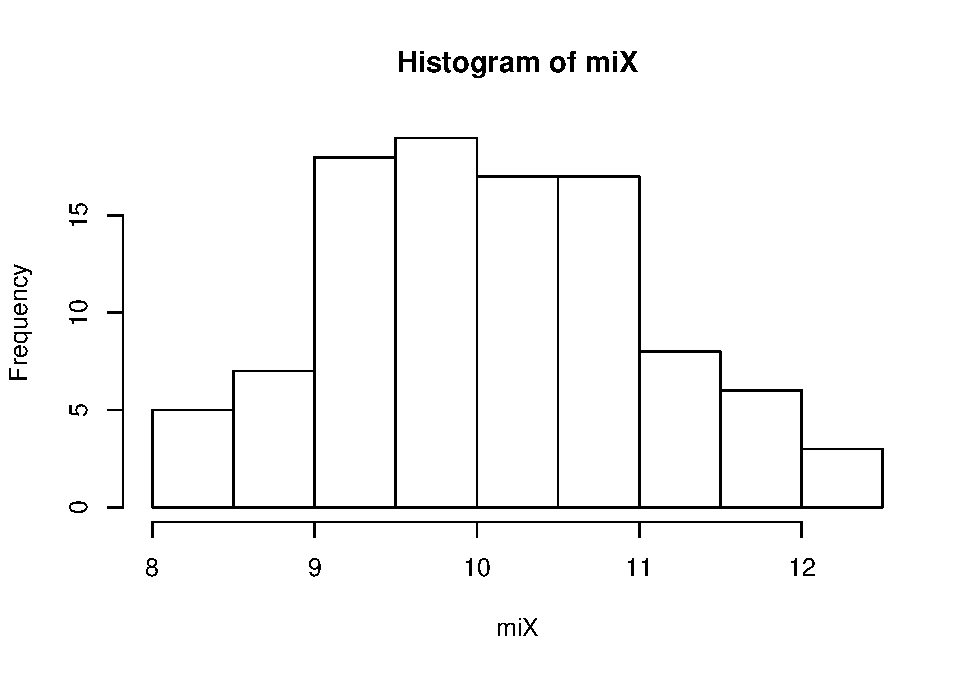
\includegraphics{R_ejercicios2021_files/figure-latex/unnamed-chunk-269-1.pdf}

El objetivo es generar mediante un loop una figura de paneles múltiples (4 filas y dos columnas), donde en cada panel se graficará un histograma con distribuciones normales de 100 valores, con media= 10. Cada figura tendrá un valor de sd definido a priori de acuerdo al vector miSD, como se muestra a continuación

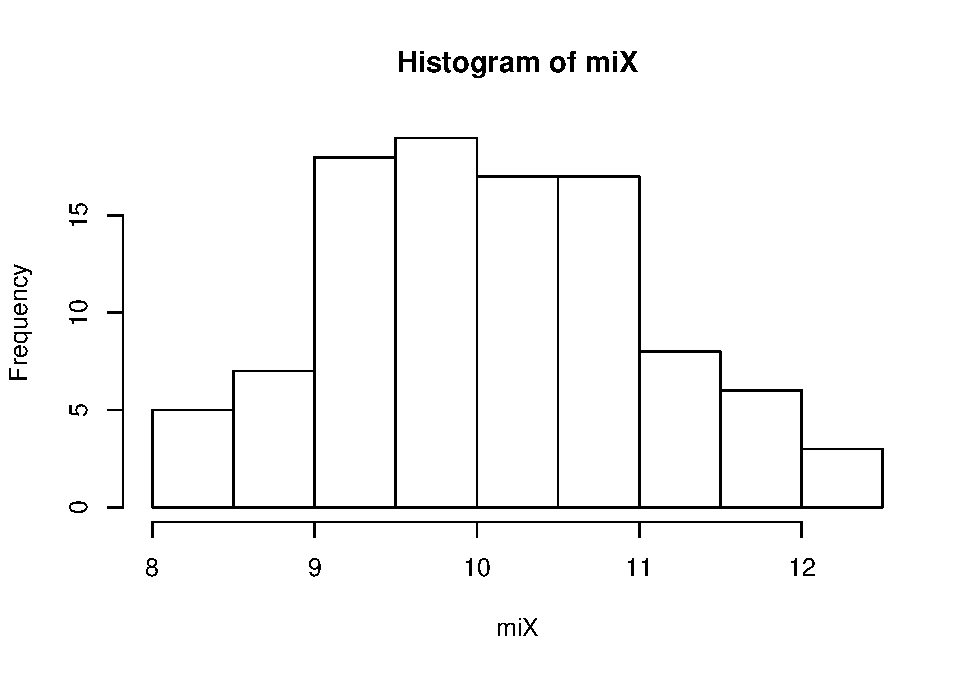
\includegraphics{R_ejercicios2021_files/figure-latex/unnamed-chunk-270-1.pdf}

Estructura

\begin{Shaded}
\begin{Highlighting}[]
\KeywordTok{set.seed}\NormalTok{(}\DecValTok{333}\NormalTok{) }\CommentTok{# definimos la semilla para que todos obtengamos los mismos números pseudoaleatorios}

\NormalTok{miSD <-}\StringTok{ }\KeywordTok{seq}\NormalTok{(}\DataTypeTok{from=} \FloatTok{0.5}\NormalTok{, }\DataTypeTok{to=} \DecValTok{4}\NormalTok{, }\DataTypeTok{by=} \FloatTok{0.5}\NormalTok{) }\CommentTok{# valores de sd que queremos evaluar}

\KeywordTok{par}\NormalTok{(}\DataTypeTok{mfrow=} \KeywordTok{c}\NormalTok{(}\DecValTok{4}\NormalTok{, }\DecValTok{2}\NormalTok{), }\DataTypeTok{mar=} \KeywordTok{c}\NormalTok{(}\DecValTok{3}\NormalTok{, }\DecValTok{1}\NormalTok{, }\DecValTok{1}\NormalTok{, }\DecValTok{1}\NormalTok{) ) }\CommentTok{#definimos los paneles y márgenes de las figuras}

  \ControlFlowTok{for}\NormalTok{ (i }\ControlFlowTok{in}\NormalTok{ miSD)\{}
\NormalTok{    miX <-}\StringTok{ }\KeywordTok{rnorm}\NormalTok{( }\DecValTok{100}\NormalTok{, }\DecValTok{10}\NormalTok{, }\DataTypeTok{sd=}\NormalTok{ COMPLETAR )}
    \KeywordTok{hist}\NormalTok{(miX, }\DataTypeTok{main=} \StringTok{""}\NormalTok{, }\DataTypeTok{ylab=}\StringTok{""}\NormalTok{, }\DataTypeTok{xlim=} \KeywordTok{c}\NormalTok{(}\OperatorTok{-}\DecValTok{5}\NormalTok{, }\DecValTok{30}\NormalTok{))}
\NormalTok{    \}}
\end{Highlighting}
\end{Shaded}

\hypertarget{figura-muxfaltiple-con-leyenda-rrr}{%
\section{Figura múltiple con leyenda (RRR)}\label{figura-muxfaltiple-con-leyenda-rrr}}

Dado que usamos par(mfrow) en el ejercicio anterior sabemos que los valores de sd se fueron completando por filas. Pero el lector, reviewer, etc. no tiene acceso al script. ¿Que tal si en cada figura agregamos una leyenda con el valor de sd utilizado?. El resultado debería verse como en la siguiente figura

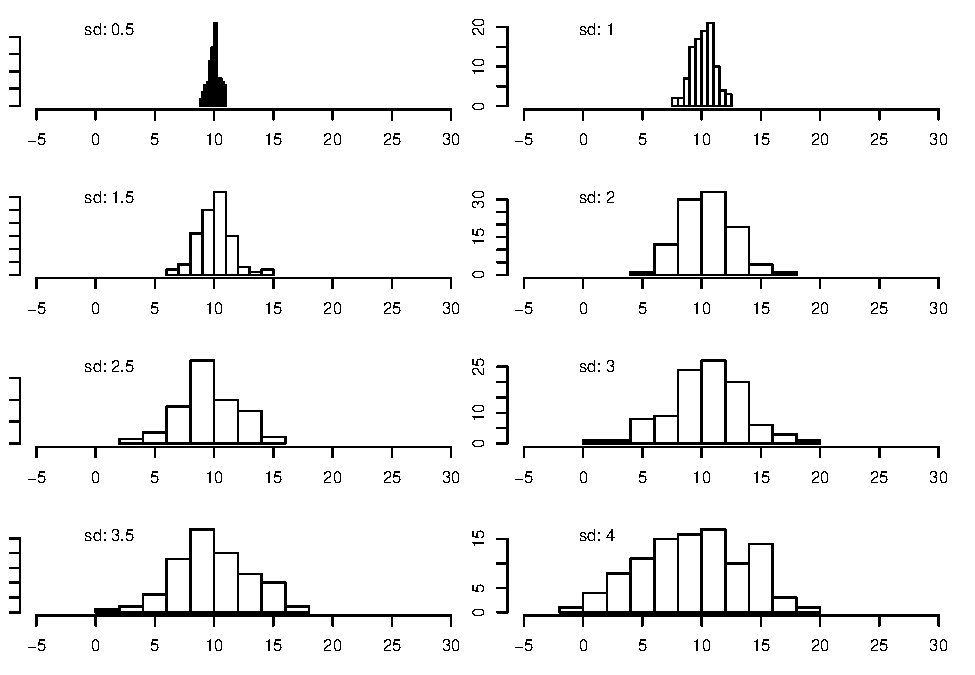
\includegraphics{R_ejercicios2021_files/figure-latex/unnamed-chunk-272-1.pdf}

Estructura

Recordemos que con par(usr= c(0, 10, 0, 10)) reescaleamos nuestra figura para independizarnos de los valores de los ejes \emph{x} y \emph{y} (ver R10.Gráficos2)

\begin{Shaded}
\begin{Highlighting}[]
\CommentTok{## RTA}
\KeywordTok{set.seed}\NormalTok{(}\DecValTok{333}\NormalTok{)}
\NormalTok{miSD <-}\StringTok{ }\KeywordTok{seq}\NormalTok{(}\DataTypeTok{from=} \FloatTok{0.5}\NormalTok{, }\DataTypeTok{to=} \DecValTok{4}\NormalTok{, }\DataTypeTok{by=}\FloatTok{0.5}\NormalTok{)}
\KeywordTok{par}\NormalTok{(}\DataTypeTok{mfrow=} \KeywordTok{c}\NormalTok{(}\DecValTok{4}\NormalTok{,}\DecValTok{2}\NormalTok{), }\DataTypeTok{mar=} \KeywordTok{c}\NormalTok{(}\DecValTok{3}\NormalTok{, }\DecValTok{1}\NormalTok{, }\DecValTok{1}\NormalTok{, }\DecValTok{1}\NormalTok{) ) }\CommentTok{#definimos los paneles y márgenes de las figuras}

  \ControlFlowTok{for}\NormalTok{ (i }\ControlFlowTok{in}\NormalTok{ miSD)\{}
\NormalTok{    miX <-}\StringTok{ }\KeywordTok{rnorm}\NormalTok{( }\DecValTok{100}\NormalTok{, }\DecValTok{10}\NormalTok{, }\DataTypeTok{sd=}\NormalTok{ COMPLETAR )}
    \KeywordTok{hist}\NormalTok{(miX, }\DataTypeTok{main=} \StringTok{""}\NormalTok{, }\DataTypeTok{ylab=}\StringTok{""}\NormalTok{, }\DataTypeTok{xlim=} \KeywordTok{c}\NormalTok{(}\OperatorTok{-}\DecValTok{5}\NormalTok{, }\DecValTok{30}\NormalTok{))}
    \KeywordTok{par}\NormalTok{( }\DataTypeTok{usr=} \KeywordTok{c}\NormalTok{(}\DecValTok{0}\NormalTok{, }\DecValTok{10}\NormalTok{, }\DecValTok{0}\NormalTok{, }\DecValTok{10}\NormalTok{) ) }\CommentTok{## este comando redefine la escala de los ejes}
    \KeywordTok{text}\NormalTok{(}\DataTypeTok{x=} \DecValTok{2}\NormalTok{, }\DataTypeTok{y=} \DecValTok{9}\NormalTok{, }\KeywordTok{paste}\NormalTok{( COMPLETAR ) ) }\CommentTok{## este comando agrega la leyenda en x y y de acuerdo a la nueva escala definida en par(usr)}
\NormalTok{    \}}
\end{Highlighting}
\end{Shaded}

\hypertarget{efecto-de-la-varianza-rrr}{%
\section{Efecto de la varianza (RRR)}\label{efecto-de-la-varianza-rrr}}

En un modelo lineal determinístico el valor esperado de una variable dependiente (\emph{y}) en función de una variable independiente (\emph{x}) está dado por:

\[y_{i} = a + b*x_{i}\]\\
donde \(a\) y \(b\) son la ordenada al origen y la pendiente respectivamente

En un modelo estocástico se agrega un componente aleatorio. Por ejemplo, en una relación lineal puede incorporarse como un error aditivo

\[y_{i} = a + b*x + e_{i}\]\\
donde \(e_{i}\) es un error aleatorio con media 0 y varianza = sigma²

Por ejemplo, el siguiente código genera una figura de dos paneles, donde se muestra el modelo determinístico (panel superior) y un modelo estocástico con error aditivo normal, con media = 0 y sd = 3

\begin{Shaded}
\begin{Highlighting}[]
\NormalTok{  x <-}\StringTok{ }\KeywordTok{runif}\NormalTok{(}\DecValTok{100}\NormalTok{, }\DecValTok{0}\NormalTok{, }\DecValTok{100}\NormalTok{) }\CommentTok{# variable independiente}
\NormalTok{  ydet <-}\StringTok{ }\FloatTok{0.5} \OperatorTok{+}\StringTok{ }\DecValTok{3} \OperatorTok{*}\StringTok{ }\NormalTok{x }\CommentTok{# variable dependiente (modelo determinístico)}
\NormalTok{  yest <-}\StringTok{ }\FloatTok{0.5} \OperatorTok{+}\StringTok{ }\DecValTok{3} \OperatorTok{*}\StringTok{ }\NormalTok{x }\OperatorTok{+}\StringTok{ }\KeywordTok{rnorm}\NormalTok{(}\DecValTok{100}\NormalTok{, }\DecValTok{0}\NormalTok{, }\DecValTok{3}\NormalTok{) }\CommentTok{# variable dependiente (modelo estocástico)}
  
\KeywordTok{par}\NormalTok{(}\DataTypeTok{mfrow=} \KeywordTok{c}\NormalTok{(}\DecValTok{2}\NormalTok{,}\DecValTok{1}\NormalTok{), }\DataTypeTok{mar=} \KeywordTok{c}\NormalTok{(}\DecValTok{2}\NormalTok{, }\DecValTok{2}\NormalTok{, }\DecValTok{2}\NormalTok{, }\DecValTok{2}\NormalTok{), }\DataTypeTok{oma=} \KeywordTok{c}\NormalTok{(}\DecValTok{3}\NormalTok{, }\DecValTok{3}\NormalTok{, }\DecValTok{1}\NormalTok{, }\DecValTok{1}\NormalTok{) ) }
    
    \KeywordTok{plot}\NormalTok{(x, ydet, }\DataTypeTok{pch=}\DecValTok{16}\NormalTok{)}
    \KeywordTok{abline}\NormalTok{(}\DataTypeTok{a=} \FloatTok{0.5}\NormalTok{, }\DataTypeTok{b=} \DecValTok{3}\NormalTok{, }\DataTypeTok{lty=}\DecValTok{2}\NormalTok{)}
    
    \KeywordTok{plot}\NormalTok{(x, yest, }\DataTypeTok{pch=}\DecValTok{16}\NormalTok{)}
    \KeywordTok{abline}\NormalTok{(}\DataTypeTok{a=} \FloatTok{0.5}\NormalTok{, }\DataTypeTok{b=} \DecValTok{3}\NormalTok{, }\DataTypeTok{lty=}\DecValTok{2}\NormalTok{)}
    
    \KeywordTok{mtext}\NormalTok{(}\DataTypeTok{side=} \DecValTok{2}\NormalTok{, }\StringTok{"Y"}\NormalTok{, }\DataTypeTok{outer=}\NormalTok{ T)}
    \KeywordTok{mtext}\NormalTok{(}\DataTypeTok{side=} \DecValTok{1}\NormalTok{, }\StringTok{"X"}\NormalTok{, }\DataTypeTok{outer=}\NormalTok{ T)}
\end{Highlighting}
\end{Shaded}

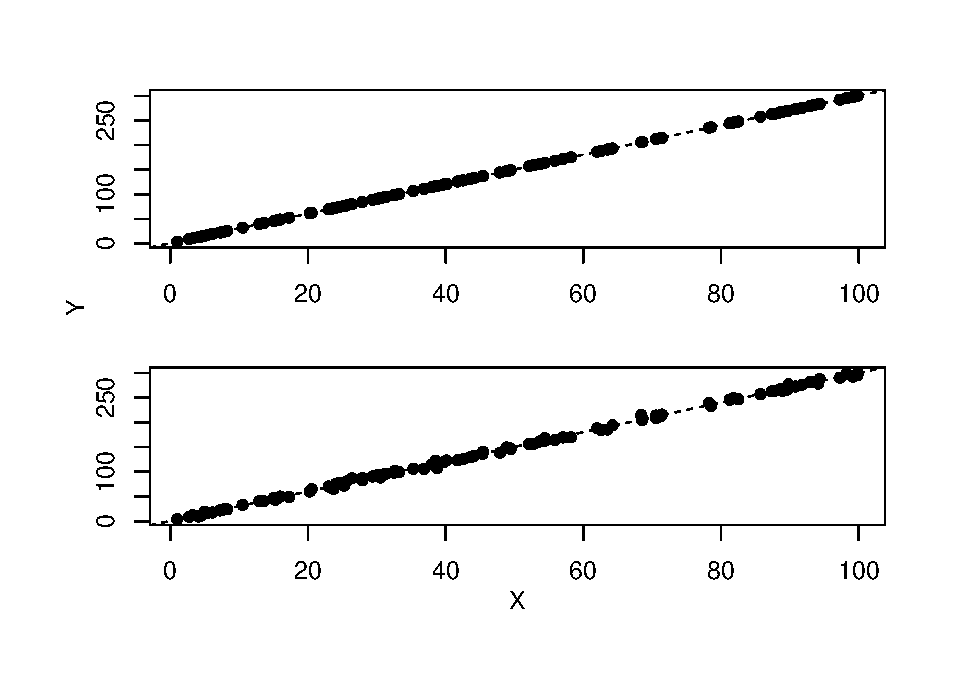
\includegraphics{R_ejercicios2021_files/figure-latex/unnamed-chunk-274-1.pdf}

El ejercicio consiste en generar un loop para evaluar el efecto de sd en la dispersión de los datos alrededor del valor medio de y. El objetivo es generar una figura múltiple como la que se muestra a continuación

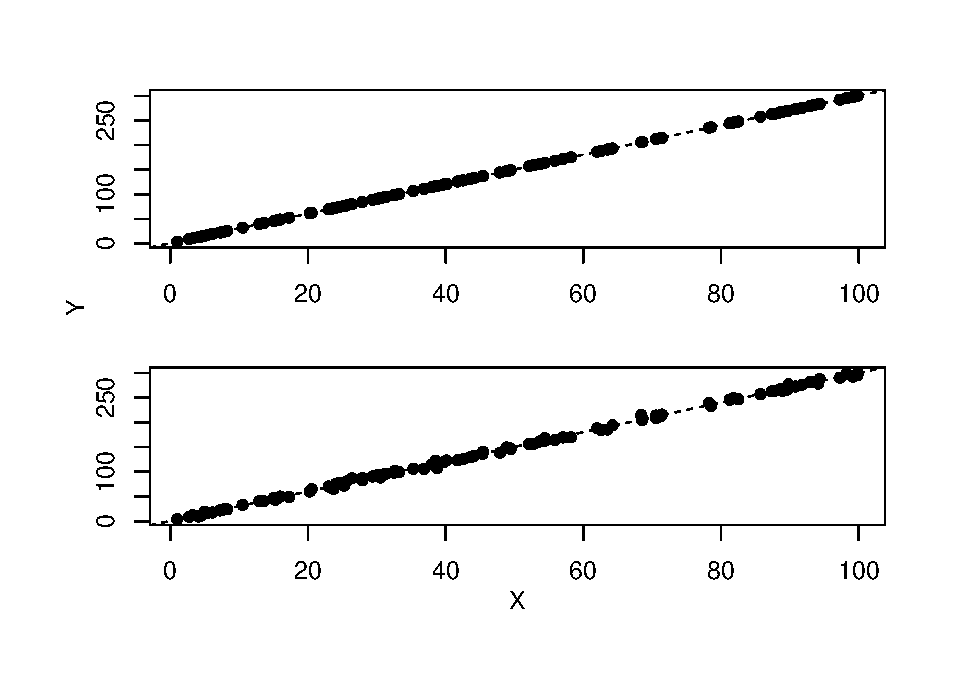
\includegraphics{R_ejercicios2021_files/figure-latex/unnamed-chunk-275-1.pdf}

Estructura

\begin{Shaded}
\begin{Highlighting}[]
\NormalTok{var =}\StringTok{ }\KeywordTok{c}\NormalTok{(}\DecValTok{1}\NormalTok{, }\DecValTok{10}\NormalTok{, }\DecValTok{30}\NormalTok{, }\DecValTok{60}\NormalTok{, }\DecValTok{90}\NormalTok{, }\DecValTok{120}\NormalTok{)}

\KeywordTok{par}\NormalTok{(}\DataTypeTok{mfrow=} \KeywordTok{c}\NormalTok{(}\DecValTok{3}\NormalTok{,}\DecValTok{2}\NormalTok{), }\DataTypeTok{mar=} \KeywordTok{c}\NormalTok{(}\DecValTok{2}\NormalTok{, }\DecValTok{2}\NormalTok{, }\DecValTok{2}\NormalTok{, }\DecValTok{2}\NormalTok{), }\DataTypeTok{oma=} \KeywordTok{c}\NormalTok{(}\DecValTok{3}\NormalTok{, }\DecValTok{3}\NormalTok{, }\DecValTok{1}\NormalTok{, }\DecValTok{1}\NormalTok{) )}

\ControlFlowTok{for}\NormalTok{(i }\ControlFlowTok{in}\NormalTok{ COMPLETAR) \{}

\NormalTok{  y <-}\StringTok{ }\FloatTok{0.5} \OperatorTok{+}\StringTok{ }\DecValTok{3} \OperatorTok{*}\StringTok{ }\NormalTok{x }\OperatorTok{+}\StringTok{ }\KeywordTok{rnorm}\NormalTok{(}\DecValTok{100}\NormalTok{, }\DecValTok{0}\NormalTok{, COMPLETAR) }
  \KeywordTok{plot}\NormalTok{(x, y, }\DataTypeTok{pch=} \DecValTok{16}\NormalTok{)}
  \KeywordTok{abline}\NormalTok{(}\DataTypeTok{a=} \FloatTok{0.5}\NormalTok{, }\DataTypeTok{b=} \DecValTok{3}\NormalTok{, }\DataTypeTok{lty=}\DecValTok{2}\NormalTok{)}
    \KeywordTok{par}\NormalTok{( }\DataTypeTok{usr =} \KeywordTok{c}\NormalTok{(}\DecValTok{0}\NormalTok{, }\DecValTok{10}\NormalTok{, }\DecValTok{0}\NormalTok{,}\DecValTok{10}\NormalTok{) )}
    \KeywordTok{text}\NormalTok{( }\KeywordTok{paste}\NormalTok{(COMPLETAR), }\DataTypeTok{x=} \DecValTok{2}\NormalTok{, }\DataTypeTok{y=} \DecValTok{8}\NormalTok{)}
\NormalTok{\}}
\KeywordTok{mtext}\NormalTok{(}\DataTypeTok{side=} \DecValTok{2}\NormalTok{, }\StringTok{"Y"}\NormalTok{, }\DataTypeTok{outer=}\NormalTok{ T)}
\KeywordTok{mtext}\NormalTok{(}\DataTypeTok{side=} \DecValTok{1}\NormalTok{, }\StringTok{"X"}\NormalTok{, }\DataTypeTok{outer=}\NormalTok{ T)}
\end{Highlighting}
\end{Shaded}

\hypertarget{figuras-muxfaltiples-rrrr}{%
\section{Figuras múltiples (RRRR)}\label{figuras-muxfaltiples-rrrr}}

Asignar a un objeto que llamaremos \textbf{\emph{env}} la tabla contenida en el archivos DoubsEnv.csv, que se encuentra en la carpeta 4-Datos (la descripción de la base de datos se encuentra en el archivo \url{datos_eer.html}).

Hemos visto que mediante el siguiente código podemos generar una figura múltiple de las variables ambientales de env

\begin{Shaded}
\begin{Highlighting}[]
\KeywordTok{par}\NormalTok{(}\DataTypeTok{mfrow=} \KeywordTok{c}\NormalTok{(}\DecValTok{5}\NormalTok{, }\DecValTok{2}\NormalTok{), }\DataTypeTok{mar=} \KeywordTok{c}\NormalTok{(}\DecValTok{3}\NormalTok{, }\DecValTok{2}\NormalTok{, }\DecValTok{2}\NormalTok{, }\DecValTok{2}\NormalTok{))}
\KeywordTok{apply}\NormalTok{(env[ , }\DecValTok{5}\OperatorTok{:}\DecValTok{14}\NormalTok{], }\DecValTok{2}\NormalTok{, hist, }\DataTypeTok{main=} \StringTok{""}\NormalTok{, }\DataTypeTok{col=} \StringTok{"grey"}\NormalTok{)}
\end{Highlighting}
\end{Shaded}

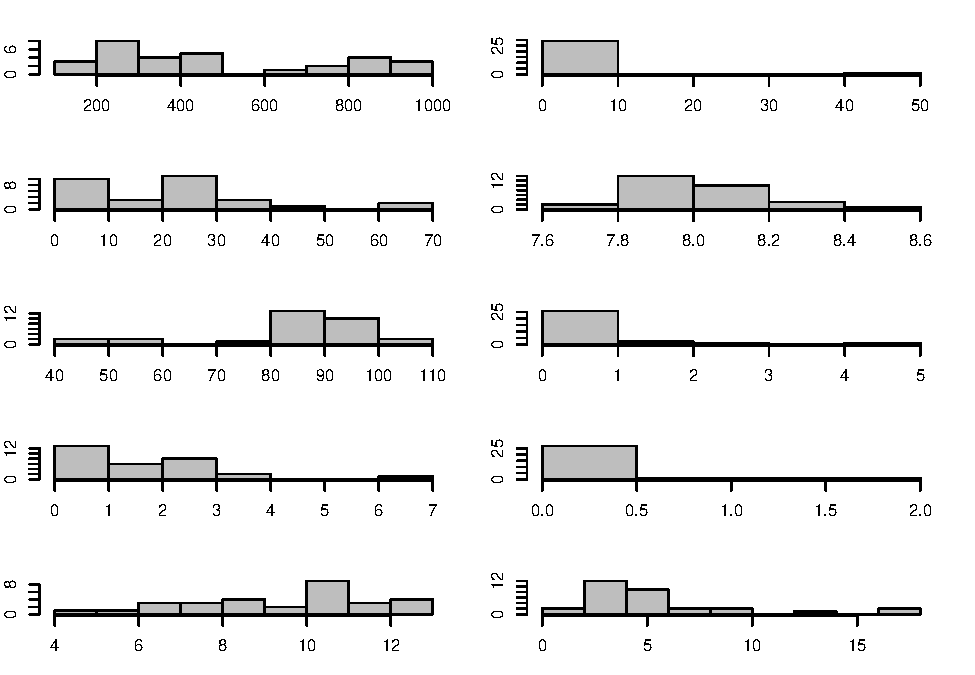
\includegraphics{R_ejercicios2021_files/figure-latex/unnamed-chunk-278-1.pdf}

Sin embargo nos gustaría poder personalizar más la figura. Por ejemplo, agregando el nombre de las variables (en castellano y sin abreviar) y opcionalmente una letra que identifique cada gráfico dentro de la figura general. Recurriremos al uso de un loop para generarlo

Lineamientos\\
* Hacer un subset del objeto env con las columnas 5:14\\
* Generar un vector con los nombres de las variables (en castellano), como se muestra más abajo\\
* Dar las opciones del par() para la figura múltiple\\
* Definir las condiciones iniciales del loop ( for i in \ldots{} )\\
* Seleccionar la columna de la variable de la iteración correspondiente\\
* Realizar el histograma\\
* Agregar el texto\\
* Fin del loop\\
* Leyenda ``Frecuencia'' en el eje y, común a todos los gráficos

\begin{Shaded}
\begin{Highlighting}[]
\NormalTok{variables <-}\StringTok{ }\KeywordTok{c}\NormalTok{(}\StringTok{"Altura"}\NormalTok{, }\StringTok{"Pendiente"}\NormalTok{, }\StringTok{"Descarga"}\NormalTok{, }\StringTok{"pH"}\NormalTok{, }\StringTok{"Dureza"}\NormalTok{, }\StringTok{"Fosfato"}\NormalTok{, }\StringTok{"Nitrato"}\NormalTok{, }\StringTok{"Amonio"}\NormalTok{, }\StringTok{"oxígeno"}\NormalTok{, }\StringTok{"Oxígeno disuelto"}\NormalTok{)}

\NormalTok{subEnv <-}\StringTok{  }\CommentTok{### subset de env con todas las filas y las columnas 5:14}
\KeywordTok{par}\NormalTok{( }\DataTypeTok{mfrow=} \KeywordTok{c}\NormalTok{(}\DecValTok{5}\NormalTok{, }\DecValTok{2}\NormalTok{), }\DataTypeTok{mar=} \KeywordTok{c}\NormalTok{(}\DecValTok{4}\NormalTok{, }\DecValTok{2}\NormalTok{, }\DecValTok{1}\NormalTok{, }\DecValTok{1}\NormalTok{), }\DataTypeTok{oma=} \KeywordTok{c}\NormalTok{(}\DecValTok{2}\NormalTok{, }\DecValTok{3}\NormalTok{, }\DecValTok{1}\NormalTok{, }\DecValTok{1}\NormalTok{) )}
   \ControlFlowTok{for}\NormalTok{(i }\ControlFlowTok{in}\NormalTok{ ....)\{}
\NormalTok{     tg <-}\StringTok{ }\CommentTok{# un objeto con la columna i de subEnv}
\StringTok{     }\KeywordTok{hist}\NormalTok{(tg, .......) }\CommentTok{# entre los argumentos debería estar el nombre de la variable i}
     \KeywordTok{par}\NormalTok{( }\KeywordTok{usr}\NormalTok{(.....) )}
     \KeywordTok{text}\NormalTok{( ...... ) }\CommentTok{# entre los argumentos debería estar la letra (a, b c, d, etc.) correspondiente a la variable i}
\NormalTok{     \}}
  \KeywordTok{mtext}\NormalTok{(.....) }\CommentTok{# leyenda del eje Y "Frecuencia"}
\end{Highlighting}
\end{Shaded}

\hypertarget{multiples-archivos-gruxe1ficos-rrrr}{%
\section{Multiples archivos gráficos (RRRR)}\label{multiples-archivos-gruxe1ficos-rrrr}}

Re diseñar el loop del ejercicio anterior, pero en vez de generar una figura múltiple se deberá guardar el histograma de cada una de las variables como archivo de imagen (jpg). El nombre de la variable deberá estar compuesto por el siguiente código: hist\_variable\emph{i}.jpg. Donde variable\emph{i} es el nombre de la variable correspondiente a la iteración \emph{i}

\hypertarget{helping-bart-rrr}{%
\section{Helping Bart (RRR)}\label{helping-bart-rrr}}

La siguiente figura muestra la típica penitencia aplicada a Bart Simpson
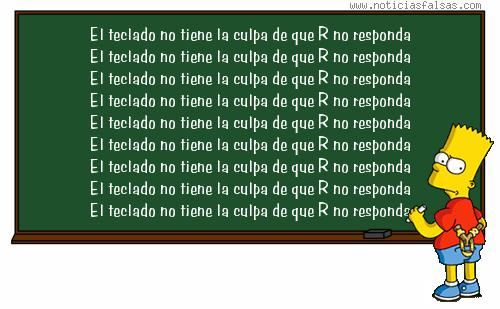
\includegraphics[width=4.16667in,height=3.75in]{figuras/bart_33.jpeg}

\end{document}
